\chapter{Results}
\label{chap:results}




\section{Experimental Setup}
\label{sec:input_data}


For the evaluation of the algorithm a suitable data set of a setup with a simple object with a smooth, organic surface was chosen. The following data set '\code{exp0040\_Carina\_\-PhantomGelatineOlive\-\_mitHalterung}' fulfils these requirements. The acquired data resulted from an \ac{usct} measurement of an olive inside a gelatin block. For the imaging a gelatin block with an olive was placed into the \ac{usct} device. 
The measurement setup can be seen in Figure \ref{fig:gelatine_setup}:


\begin{figure}[H]
     \centering
     \begin{subfigure}[b]{0.49\textwidth}
         \centering
         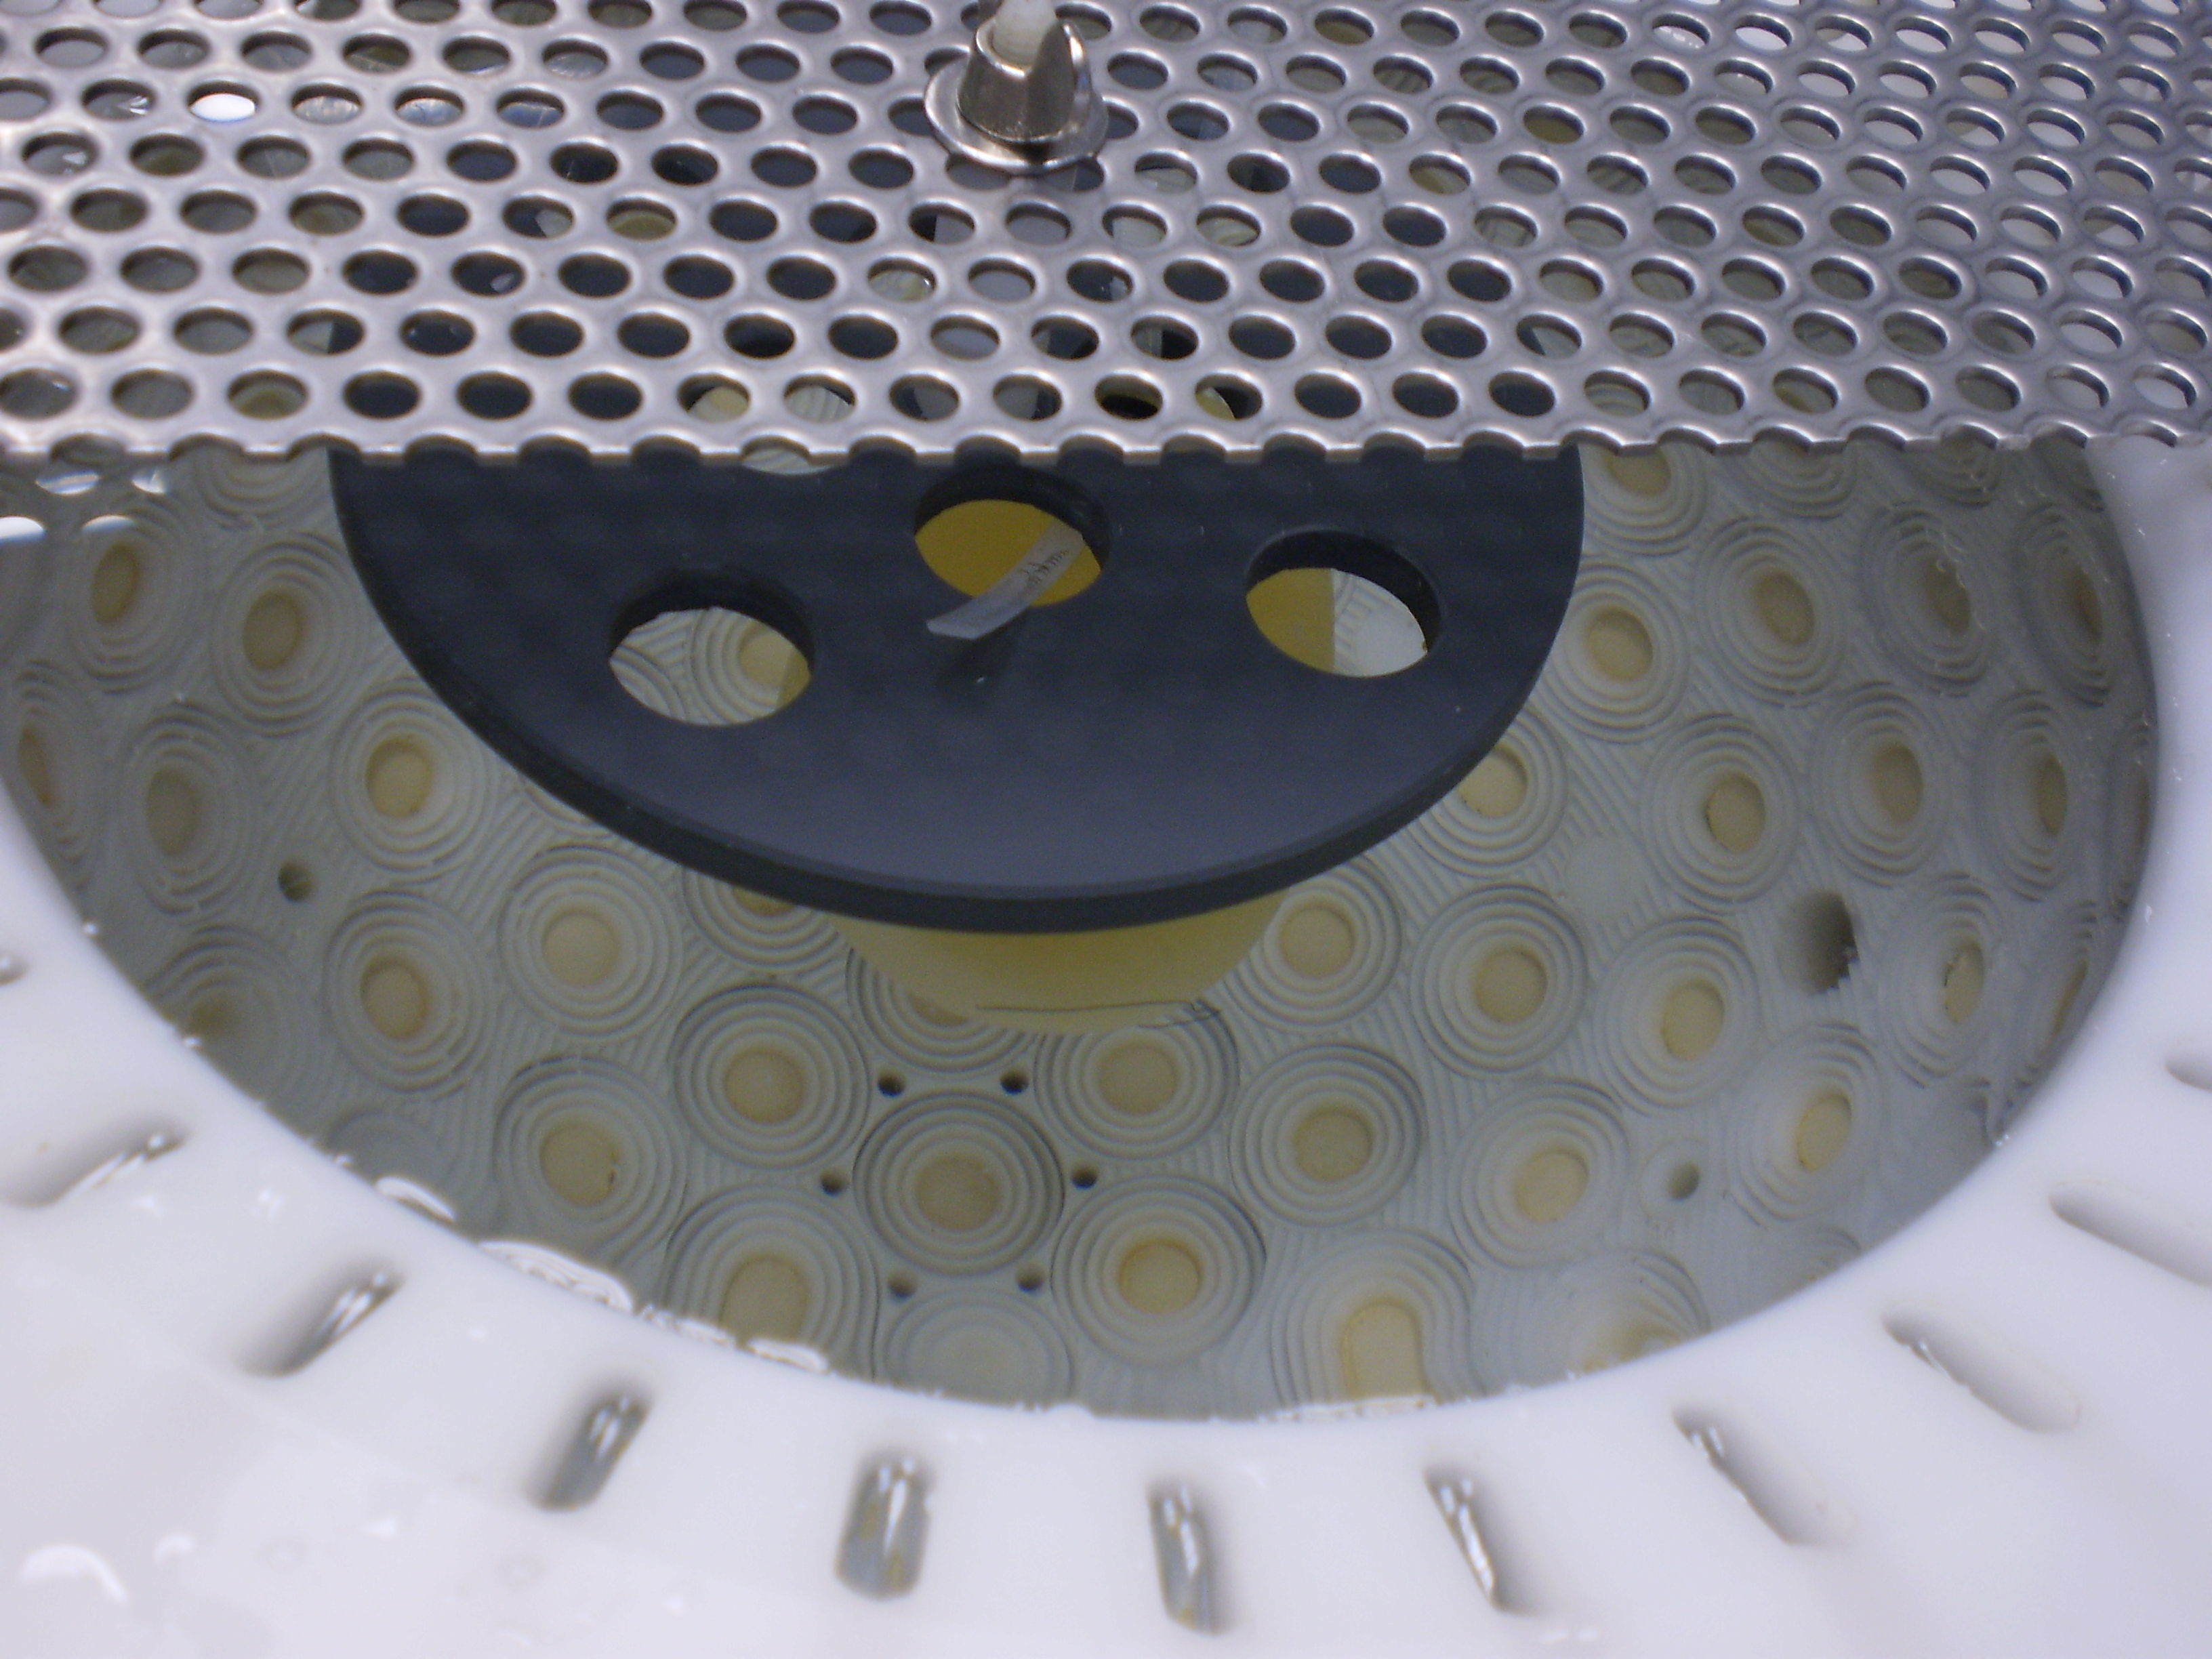
\includegraphics[width=0.99\textwidth]{Graphics/gelatin_setup1.JPG}
         \caption{Gelatin block in the imaging aperture of the \ac{usct} device.}
         \label{fig:gelatine_setup_2}
     \end{subfigure}
     \hfill
     \begin{subfigure}[b]{0.49\textwidth}
         \centering
         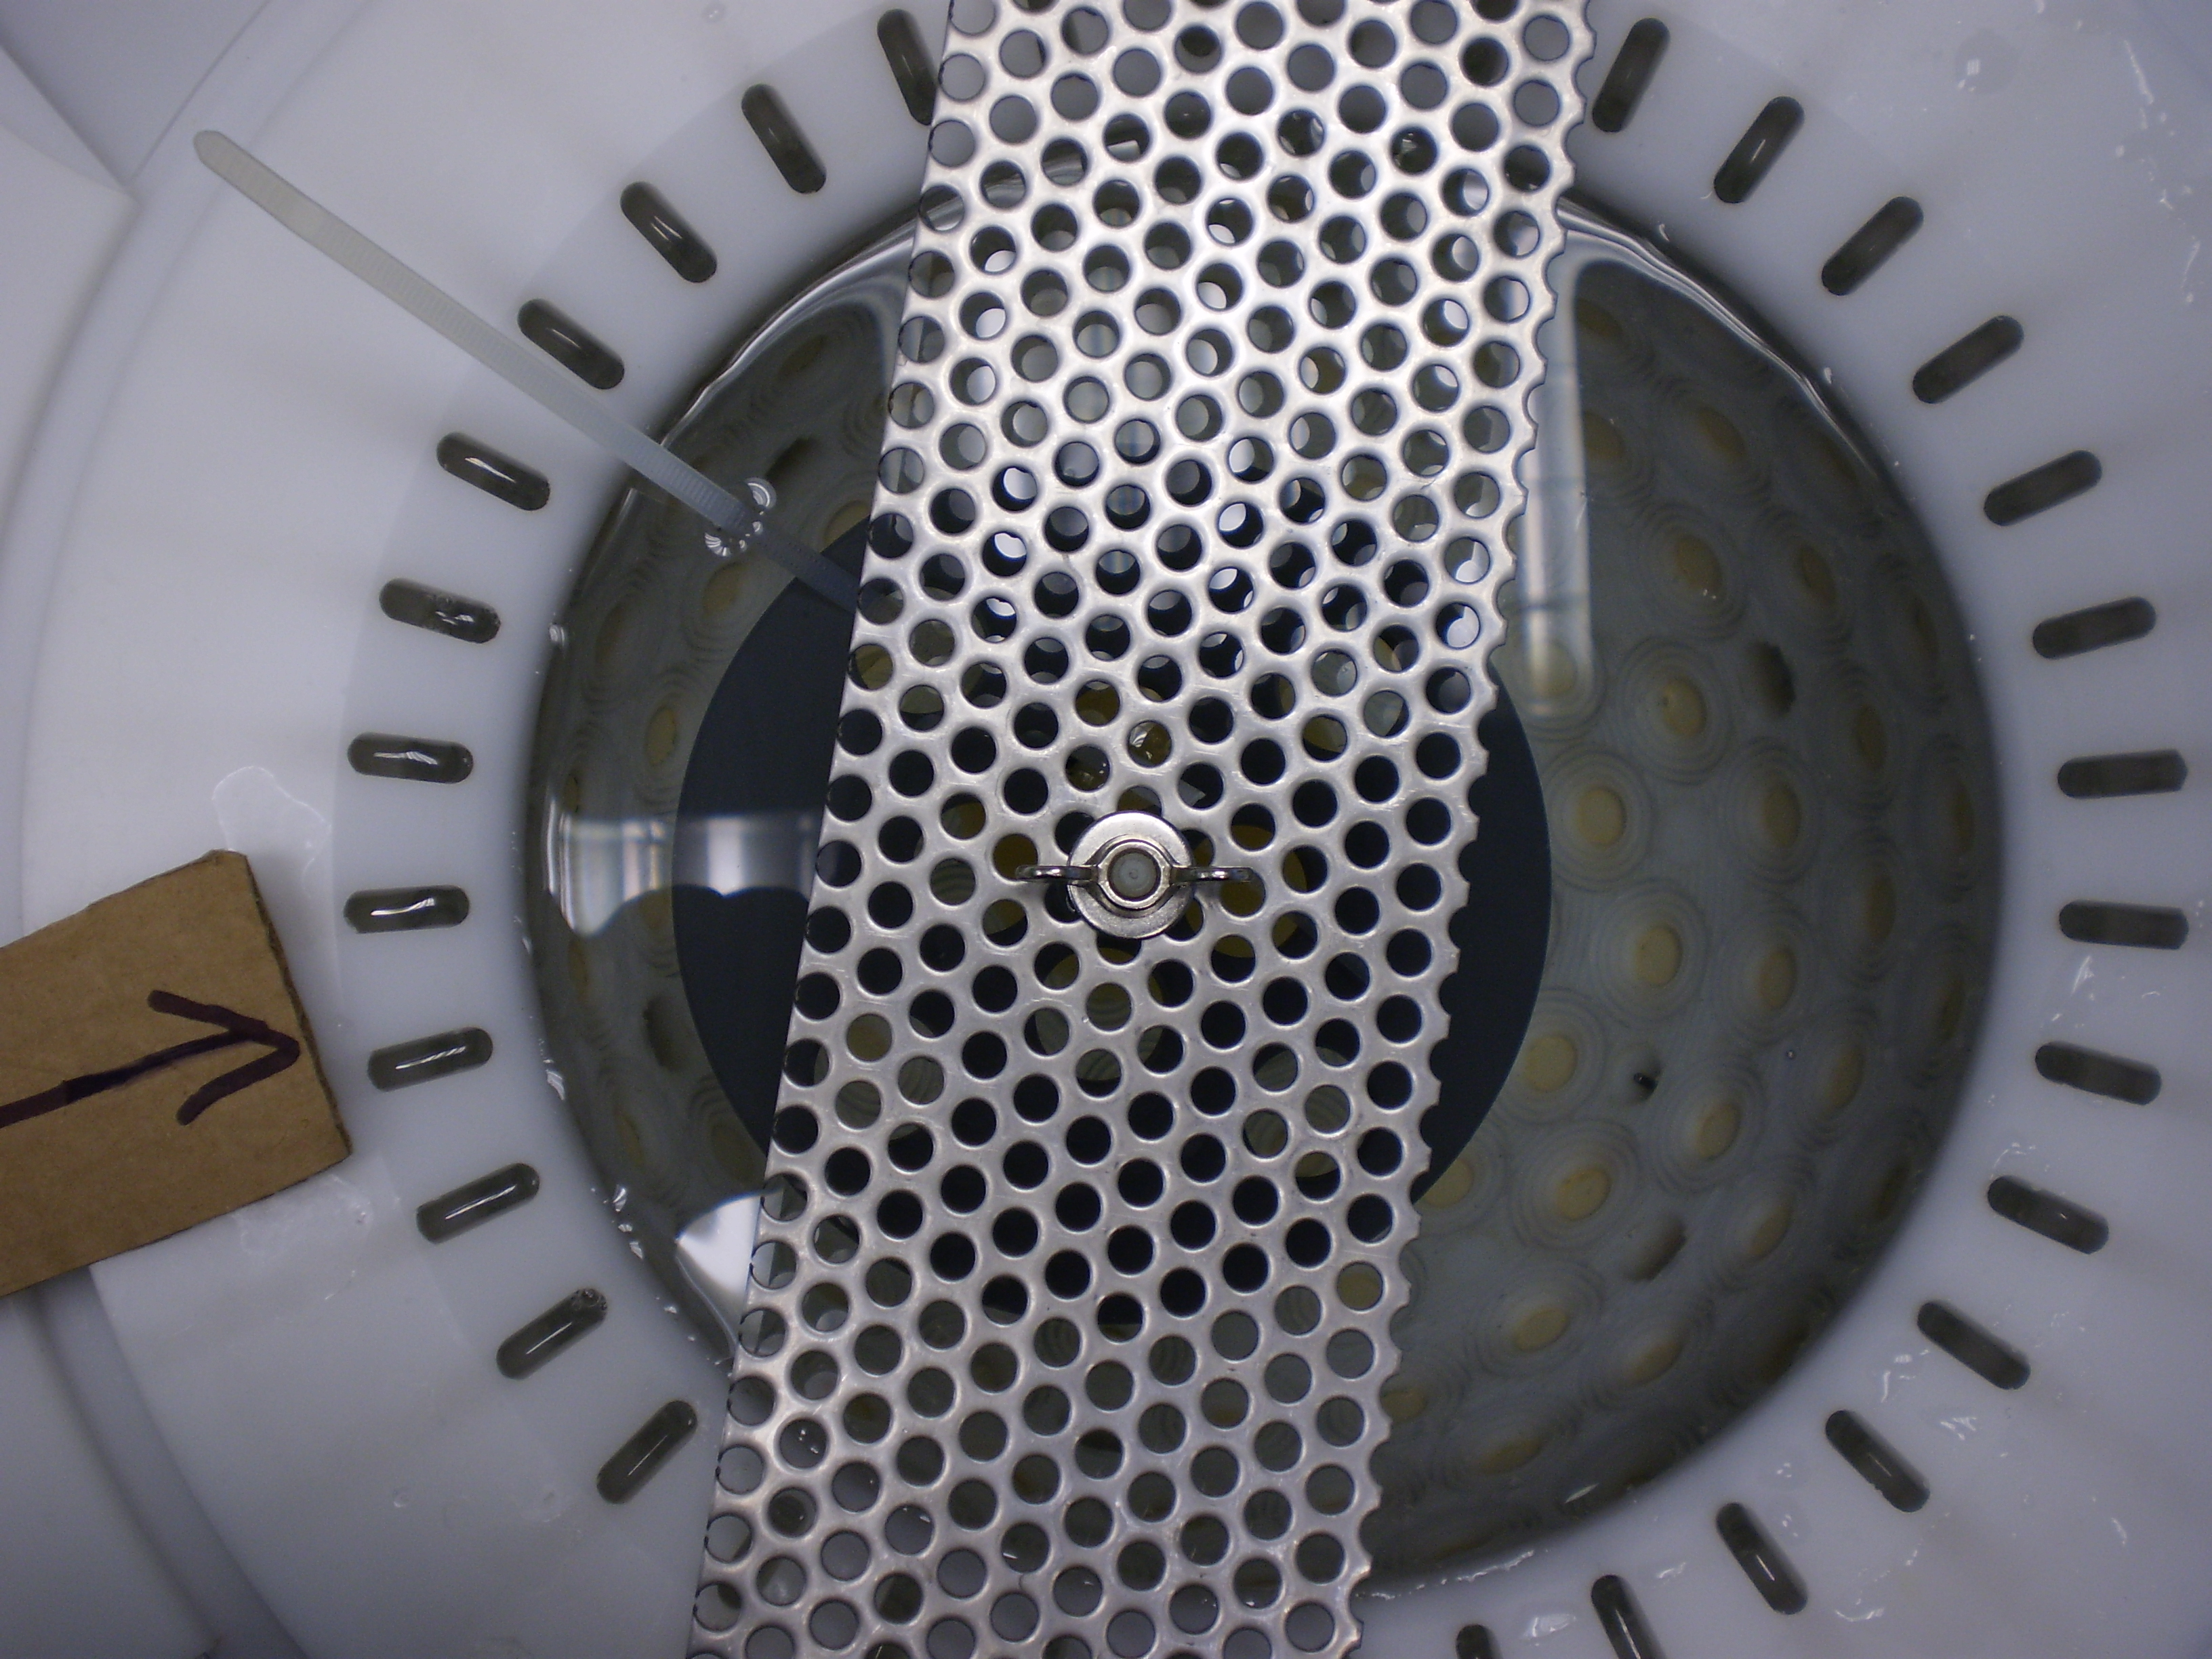
\includegraphics[width=0.99\textwidth]{Graphics/gelatin_setup 2.JPG}
         \caption{View from the top.}
         \label{fig:gelatine_setup_1}
     \end{subfigure}
        \caption{Measurement setup of the gelatin block with olive inside of the \ac{usct} device.}
        \label{fig:gelatine_setup}
\end{figure}


The \acp{ascan} were recorded for all 157 \ac{tas} with ten aperture positions so a total of $157\cdot4\cdot157\cdot9\cdot10 = 8.8\cdot10^6$ \acp{ascan} were recorded. The reconstructed reflection image for this data set is shown in Figure \ref{fig:res:reflec_image_olive_xyz}. The sub plots each show a slice through the image. The coloured lines in each plot show the selected slice in the other two coordinate systems. The blue marker belongs to the z-dimension, the green one corresponds to the y-dimension and therefore the red marker shows the x-dimension. Figure \ref{fig:res:reflec_image_olive_xyz_x} shows the x-layer for $x = 0$. That x is equal to zero can be seen in the other two figures where the red markers are located at about 0. Analogously, Figure \ref{fig:res:reflec_image_olive_xyz_y} and  \ref{fig:res:reflec_image_olive_xyz_z} show the y-layer and z-layer of the image.

\begin{figure}[H]
     \centering
     \begin{subfigure}[b]{0.49\textwidth}
         \centering
        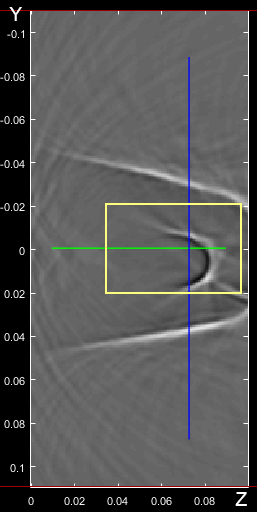
\includegraphics[width=0.59\linewidth]{Graphics/Results/Olive_Standart_reco_example/olive_standart_reconstruction_whole_volume_x_layer.png}
         \caption{x-Layer}
         \label{fig:res:reflec_image_olive_xyz_x}
     \end{subfigure}
     \hfill
     \begin{subfigure}[b]{0.49\textwidth}
         \centering
         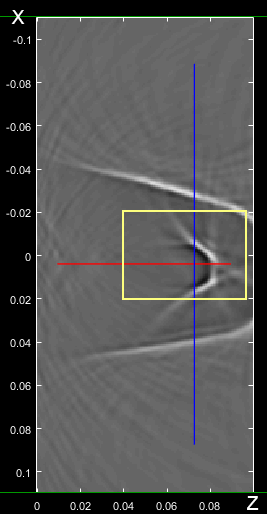
\includegraphics[width=0.61\textwidth]{Graphics/Results/Olive_Standart_reco_example/olive_standart_reconstruction_whole_volume_y_layer.png}
         \caption{y-Layer}
         \label{fig:res:reflec_image_olive_xyz_y}
     \end{subfigure}
     \hfill
     \begin{subfigure}[b]{0.55\textwidth}
         \centering
         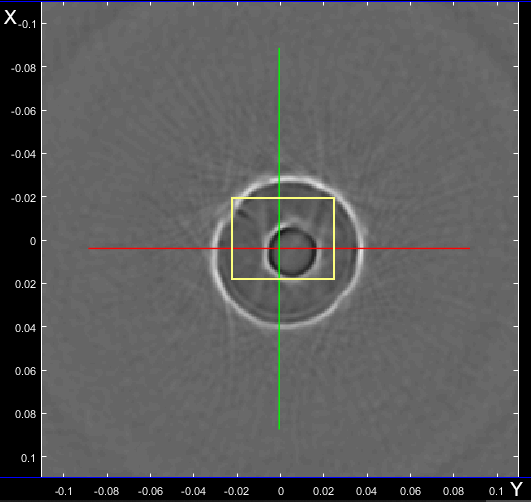
\includegraphics[width=0.99\textwidth]{Graphics/Results/Olive_Standart_reco_example/olive_standart_reconstruction_whole_volume_z_layer.png}
         \caption{z-Layer}
         \label{fig:res:reflec_image_olive_xyz_z}
     \end{subfigure}
        \caption{Reconstructed reflection image of an olive in gelatin. The yellow box marks the area that was used during the reconstructions with five dimension to limit the amount of data.
        Name of the data set: '\code{exp0040\_Carina\_PhantomGelatineOlive\_mitHalterung}'.}
        \label{fig:res:reflec_image_olive_xyz}
\end{figure}


In the centre of Figure \ref{fig:res:reflec_image_olive_xyz_z} the olive can be seen as the smaller, darker circular shape. The brighter shape around the olive is the gelatin block. 

\bigskip


The volume was only partially considered during the 5D reconstruction to reduce the amount of data that had to be processed and by that also reduce the computation time. The start point for the volume was set to $[\, -0.02,\, -0.02,\, 0.04\, ]$ and the end point was set to: $[ 0.02,\, 0.02,\, 0.095\, ]$. The utilised volume is marked with the yellow boxes in Figure \ref{fig:res:reflec_image_olive_xyz}. This particular volume was chosen to include as many different types of tissue as possible. Therefore, four particular voxels where chosen at the location of different tissue samples. The first voxel is located at $[85\, , \, 66\, , \, 87]$ at the edge of the olive. The 2\textsuperscript{nd} test voxel is located at $[18\, , \, 21\, , \, 87]$ right in the gelatin around the olive. The third voxel is located on the surface of the gelatin block at the coordinates $[1\, , \, 6\, , \, 76]$. At $[40\, , \, 60\, , \, 87]$ another voxel was chosen in the pulp of the olive. The position of these voxels can be seen in Figure \ref{fig:different_tisue_types}.  
      
      
      
\begin{figure}[H]
    \centering
    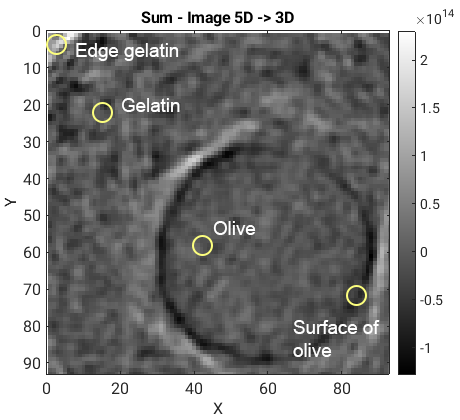
\includegraphics[width=0.76\textwidth]{Graphics/Results/Variance_Image/stone_skin_pulp_location.png}
    \caption{Overview of the reconstructed area with the location of the test voxels for the different types of material inside of the gelatin block.}
    \label{fig:different_tisue_types}
\end{figure}
    


\section{Evaluation of the assignment process during 5D reconstruction}
The introduction of the fifth dimension was explained in section \ref{chap:SAFT_Augment}. The assignment process of the  voxel value $V_k$ to the voxels in the 4\textsuperscript{th} and 5\textsuperscript{th} dimension was explained in section \ref{sec:index_ident}. The functionality of this process is shown in this section. In this example the 4\textsuperscript{th} dimension will relate to the comparison vector from the voxel to the receiver. The 5\textsuperscript{th} dimension is defined as the comparison vector from the voxel to the emitter. During the reconstruction 14 directional vectors were used. 
The configuration of active emitters and receivers is shown in Figure \ref{fig:res:5th_dim_over_4th_aperture}. The green crosses mark the location of all active receivers and the red circles represent the emitters. For this example the first 30235 \acp{ascan} are used which include the first 40 emitters and 1309 receivers. The data of every receiver that lays in a $\pm 120^{\circ}$ angle to the sender normal is included for that particular emitter. This constellation is shown in Figure \ref{fig:res:5th_dim_over_4th_aperture}.

\begin{figure}[H]
    \centering
    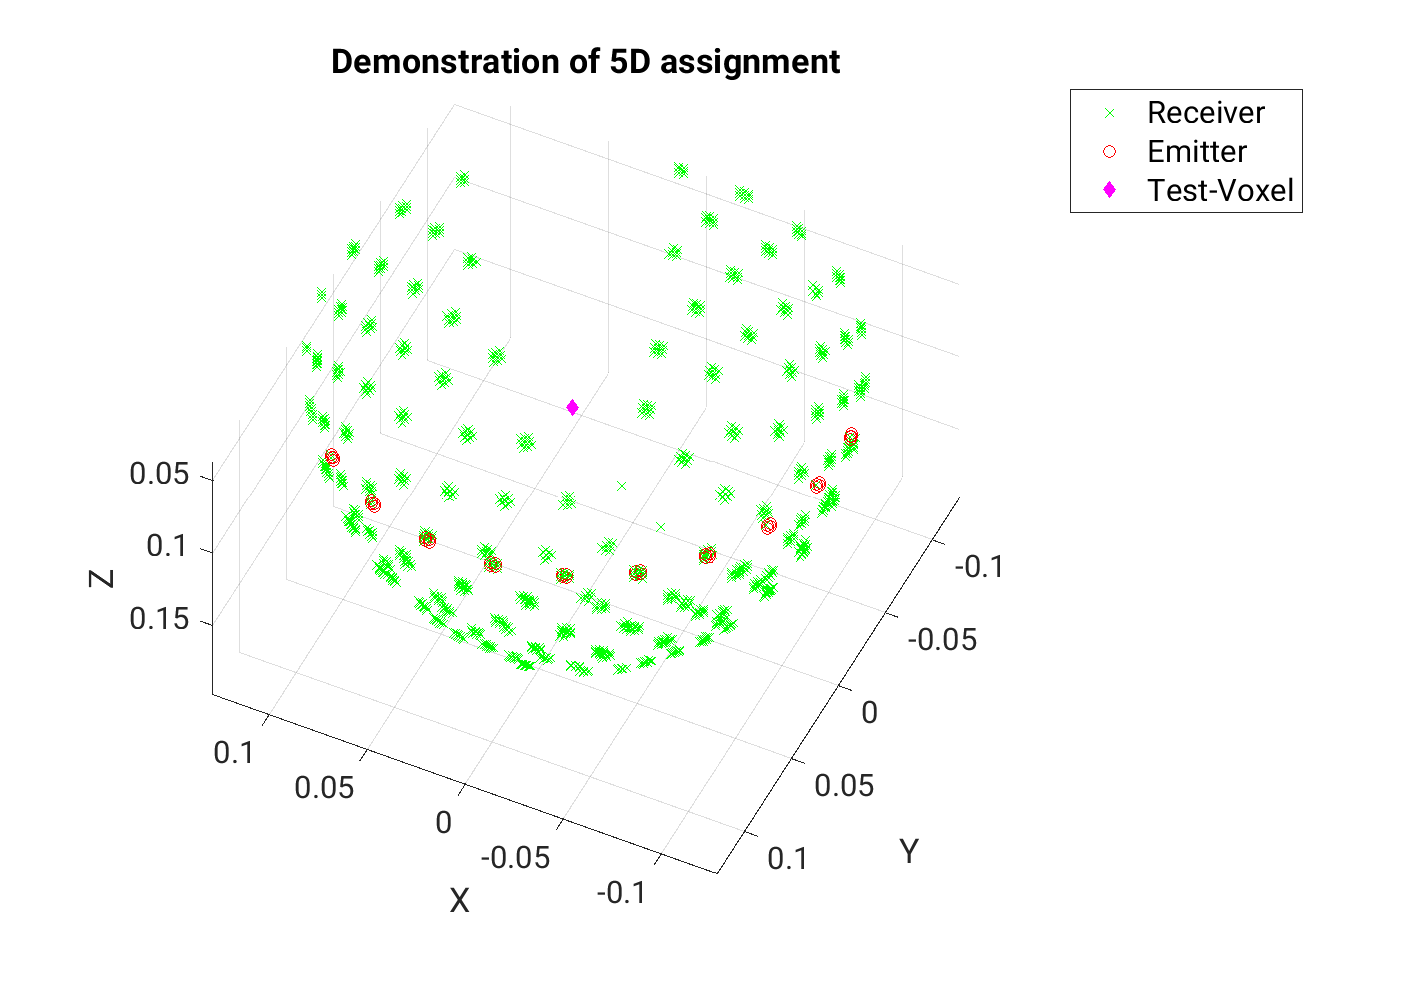
\includegraphics[width=0.89\linewidth]{Graphics/Results/4d_5d/5thDim_over_4thDim_150_150_150_apertur.eps}
    \caption{Configuration of 10 emitting and 145 receiving \ac{tas} and a test voxel in the centre of the aperture. The receivers are shown in green and the emitters as red circles. The units on the axes is given in meter. }
    \label{fig:res:5th_dim_over_4th_aperture}
\end{figure}

 For this example a test vector is defined arbitrarily in the centre of the aperture. The coordinates of this point are given by voxel indices $[150\, , \, 150\, , \, 150]$ and it is shown as the pink diamond in Figure \ref{fig:res:5th_dim_over_4th_aperture}. The coordinates of the voxel can be converted into the coordinate system of the \ac{usct} which is given in meters. The test voxel therefore is located at $[0.0047m\, , \, 0.0047m\, , \, 0.0047m]$.

 During the reconstruction the sum of each voxel value $V_k$ from the \ac{saft} for each voxel is saved in the 5D volume. The following figure shows the voxel values for the one test voxel in the centre of the aperture at the position of the pink diamond. Since there are 5 dimensions each dimensions gets assigned a certain amount of voxel values for each combination of dimensions. Every combination of the 4\textsuperscript{th} dimension with the 5\textsuperscript{th} dimension is shown in Figure \ref{fig:res:5th_dim_over_4th_result}.
 
 
\begin{figure}[H]
    \centering
    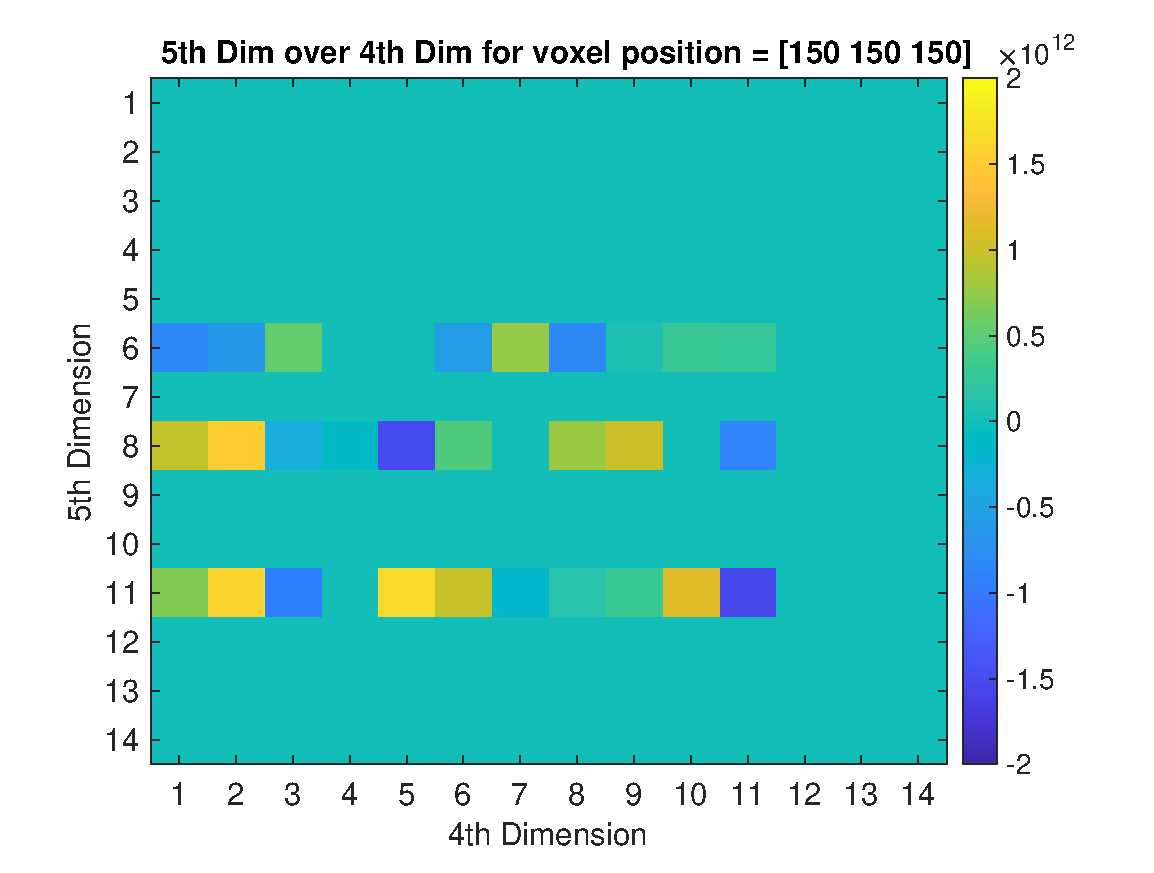
\includegraphics[width=0.89\linewidth]{Graphics/Results/4d_5d/5thDim_over_4thDim_150_150_150.eps}
    \caption{Resulting voxel values $V_k$ of the five dimensional reconstruction. The 4\textsuperscript{th} dimension relates to the voxel-receiver-vector. The 5\textsuperscript{th} dimension represents the directional information for the voxel-emitter-vector.}
    \label{fig:res:5th_dim_over_4th_result}
\end{figure}

To understand Figure \ref{fig:res:5th_dim_over_4th_result} the example of the Rubik's cubes in Figure \ref{5D_rubics} shall be used. In the previous example there were only four directional vectors. This resulted in $4 \times 4 = 16$ Rubik's cubes. In the 4\textsuperscript{th} dimension the cubes held the information about the receiver directions. The the 5\textsuperscript{th} dimension held the date for the emitters. The here shown data was generated with 14 directional vectors which leads to a $14 \times 14$ matrix with a total of 196 Rubik's cubes. These 196 Rubik's cubes are shown in Figure \ref{fig:res:5th_dim_over_4th_result} but not as whole but only the value of the voxel $[150\, , \, 150\, , \, 150]$ in each cube.
Every value that can be found in same row of the matrix in Figure \ref{fig:res:5th_dim_over_4th_result} was recorded by the same emitter. Analogously, every value in the same column belongs to the same receiver. The distribution of values in the 5D-over-4D representation is compared to the emitter-receiver-configuration from Figure \ref{fig:res:5th_4th_cones}. It shows the 14 directional vectors and their corresponding decision cones.


\begin{figure}[H]
     \centering
     \begin{subfigure}[b]{0.49\textwidth}
         \centering
        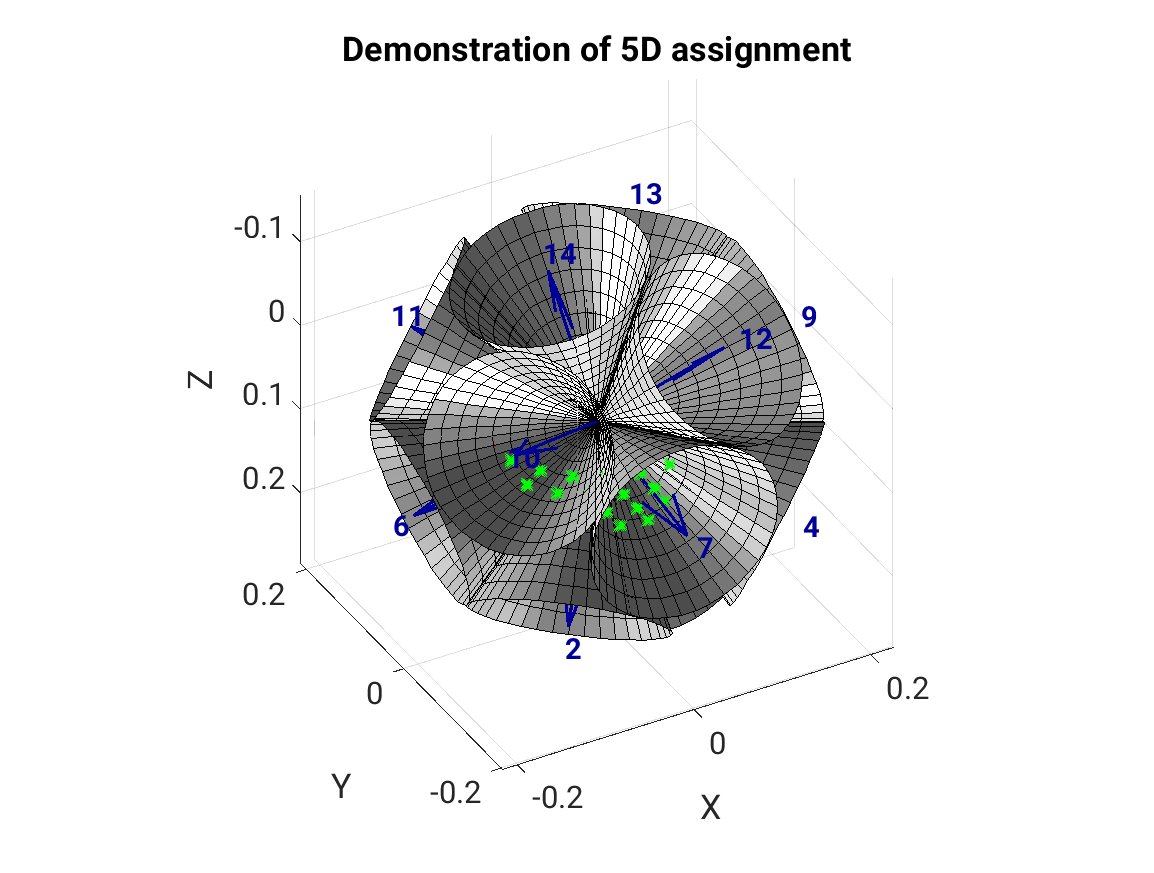
\includegraphics[width=1.3\linewidth]{Graphics/Results/4d_5d/5thDim_over_4thDim_150_150_150_cones_10_center.eps}
         \caption{Cone 10}
         \label{fig:res:5th_4th_cones10}
     \end{subfigure}
     \hfill
     \begin{subfigure}[b]{0.49\textwidth}
         \centering
         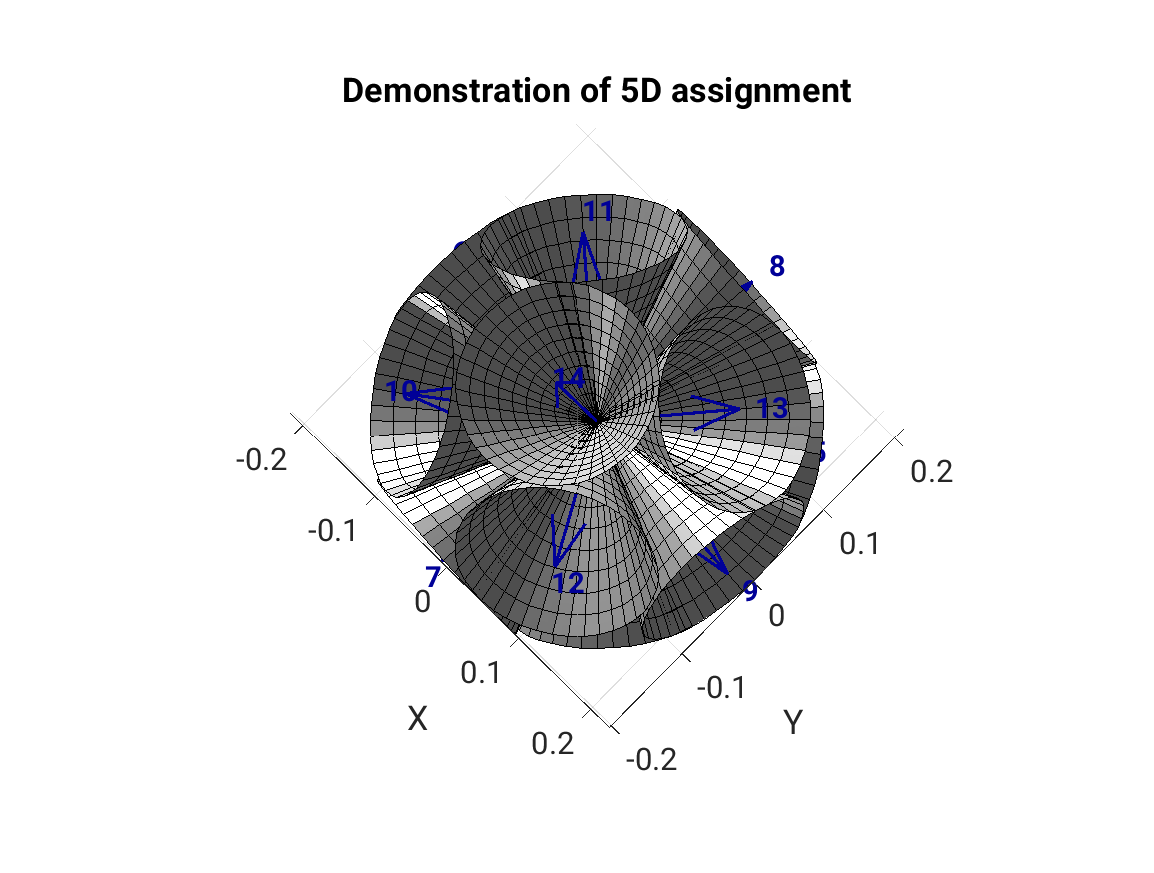
\includegraphics[width=1.3\textwidth]{Graphics/Results/4d_5d/5thDim_over_4thDim_150_150_150_cones_14_center.eps}
         \caption{Cone 14}
         \label{fig:res:5th_4th_cones14}
     \end{subfigure}
     \hfill
     \begin{subfigure}[b]{0.49\textwidth}
         \centering
         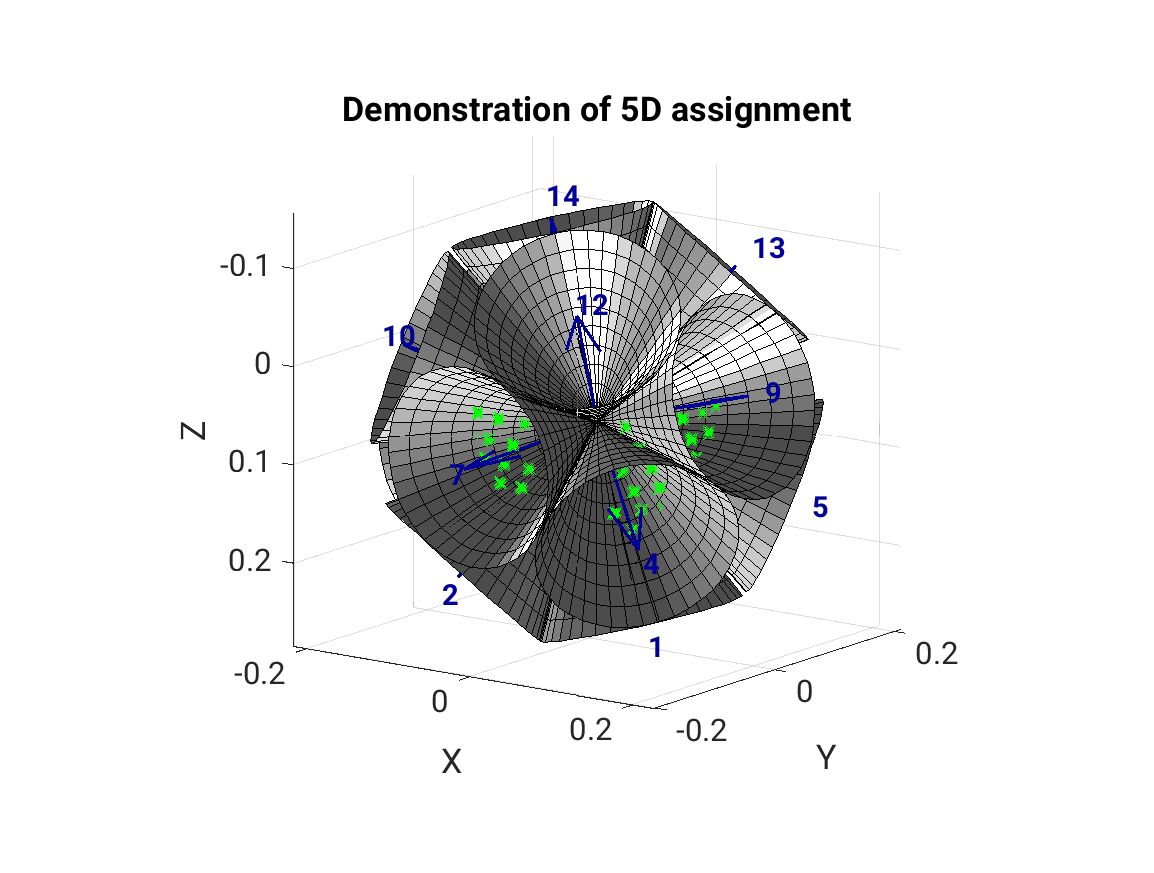
\includegraphics[width=1.3\textwidth]{Graphics/Results/4d_5d/5thDim_over_4thDim_150_150_150_cones_7_9_center.eps}
         \caption{Cone 12}
         \label{fig:res:5th_4th_cones12}
     \end{subfigure}
     \hfill
     \begin{subfigure}[b]{0.49\textwidth}
         \centering
         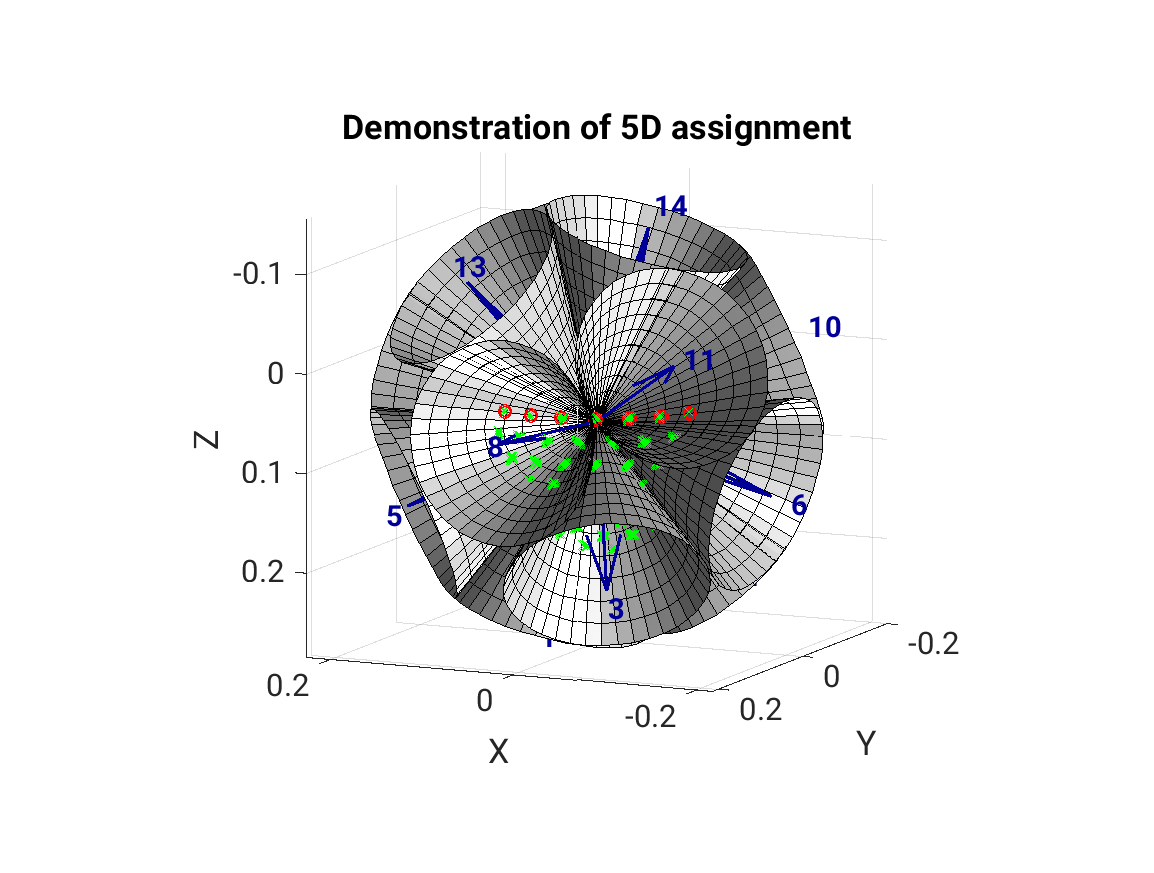
\includegraphics[width=1.3\textwidth]{Graphics/Results/4d_5d/5thDim_over_4thDim_150_150_150_cones_8_11_center.eps}
         \caption{Cone 11}
         \label{fig:res:5th_4th_cones11}
     \end{subfigure}
     \hfill
     \begin{subfigure}[b]{0.49\textwidth}
         \centering
         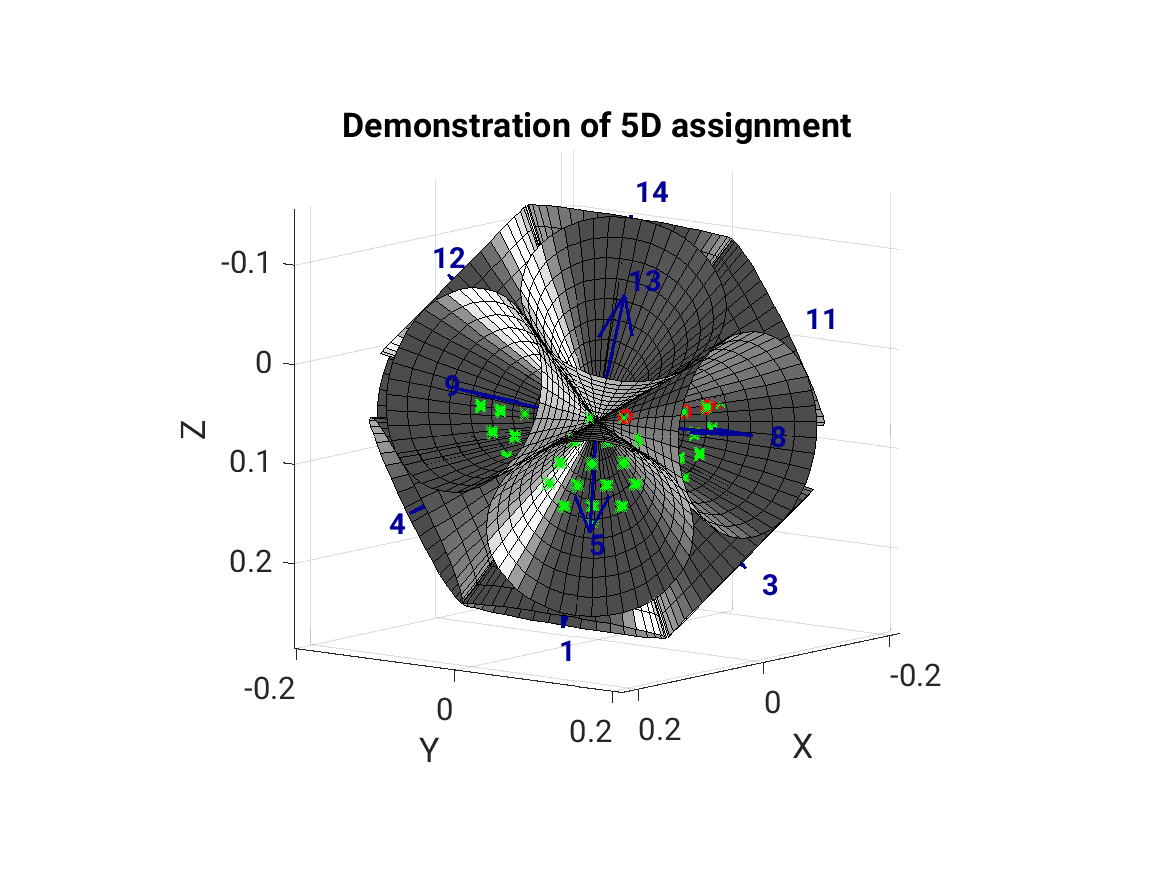
\includegraphics[width=1.3\textwidth]{Graphics/Results/4d_5d/5thDim_over_4thDim_150_150_150_cones_9_8_center.eps}
         \caption{Cone 5}
         \label{fig:res:5th_4th_cones5}
     \end{subfigure}
        \caption{The emitter receiver configuration of Figure \ref{fig:res:5th_dim_over_4th_aperture} with added directional vectors and decision cones. The origin of each cone is located at the position of the test voxel $[150\, , \, 150\, , \, 150]$. }
        \label{fig:res:5th_4th_cones}
\end{figure}

To connect the results shown in Figure \ref{fig:res:5th_dim_over_4th_result} with the cone images in Figure \ref{fig:res:5th_4th_cones} we start by looking at the red dots in the 5d-over-4d image. These red dots are representing the emitters which were active during the first set of \acp{ascan}. When the \ac{saft} is executed a voxel value $V_k$ is calculated. For this voxel value and its corresponding voxel the comparison vector from the voxel to the emitter is constructed. This voxel-emitter-comparison-vector then is assigned to the directional vectors. This is done by checking in what cone the comparison vector lands. In Figure \ref{fig:res:5th_4th_cones} for every red dot that is visible in one of the cones this means that there is a comparison vector from the test voxel $[150\, , \, 150\, , \, 150]$ to that particular emitter and it is assigned to the cone where the red emitter is visible in. In this example the following cones contain red dots: 6, 8 and 11. The results in Figure \ref{fig:res:5th_dim_over_4th_result} show, that the only the rows for 6, 8 and 11 are occupied. All other rows are empty. This coincides with the assumption that the 5\textsuperscript{th} dimension relates to the voxel-emitter-comparison-vector and that the emitters are only assigned to three directional vectors. 
For the receivers, which are plotted in green, the comparison vectors from the voxel to the receiver are relevant and the data can be found in the fourth dimension. This is why in Figure \ref{fig:res:5th_dim_over_4th_result} only the columns are occupied for that directional vectors were assigned to the green receiver dots. Figure \ref{fig:res:5th_4th_cones14} shows an example of cones where neither a red emitter nor a green receiver is located in. The empty cones in this case are 12, 13 and 14. These are the cones that point toward the opening of the aperture where no transducers are located. Therefore, it is no surprise that no data is recorded from there. In the 5D-over-4D representation of the voxel values these are the dimensions where neither the column nor the rows are occupied.

\bigskip

To verify that the image information was assigned correctly during the reconstruction, the following figure shows the sum image which was generated by summarising all values over te 4\textsuperscript{th} and 5\textsuperscript{th} dimension:


\begin{figure}[H]
    \centering
    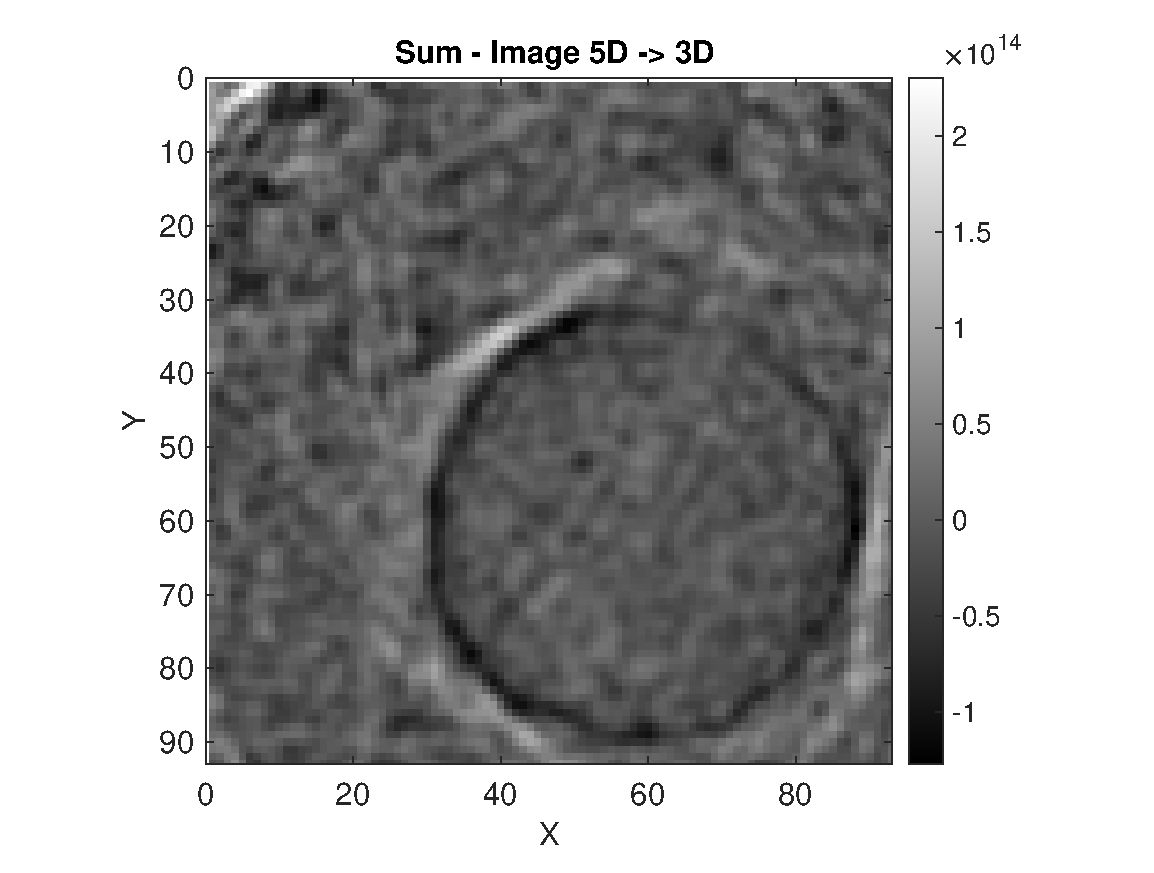
\includegraphics[width=0.69\linewidth]{Graphics/sum_image_35_vec_to_show_that_assign_works.eps}
    \caption{Sum image of the five dimensional data over the 4\textsuperscript{th} and 5\textsuperscript{th} dimension. }
    \label{fig:res:sum_image_35_vec_to_show_that_assign_works}
\end{figure}

The sum image shows the 3D image of the olive and therefore the expected outcome was reached. If something had gone wrong during the assignment of the directional information, strong visible artefacts would be expected in the sum image that would exceed the expected artefacts of the \ac{saft} image.



\section{Comparison of orthogonality threshold method and angle sorting method}

In section \ref{sec:index_ident} two methods for the assignment of comparison vectors to the right directional vector were explained. It was also mentioned that both methods have different decision regions for the directional vectors. The influence of these differences is shown in this section. In the following all images were created using 25 directional vectors and with the added 4\textsuperscript{th} dimension which stores the information about the voxel-receiver relation. The reason for not also including the 5\textsuperscript{th} dimension was to keep the computation time as small as possible and still being able indicate the differences in the resulting images. The following Figure \ref{fig:res:slice_diff_bubble_ortho_image} shows a side by side comparison of the reflection image for both assignment methods. From the 4D image the following images are from the 3\textsuperscript{rd} directional vector and the 166\textsuperscript{th} slice in the z-dimension.


\begin{figure}[H]
     \centering
     \begin{subfigure}[b]{0.49\textwidth}
         \centering
        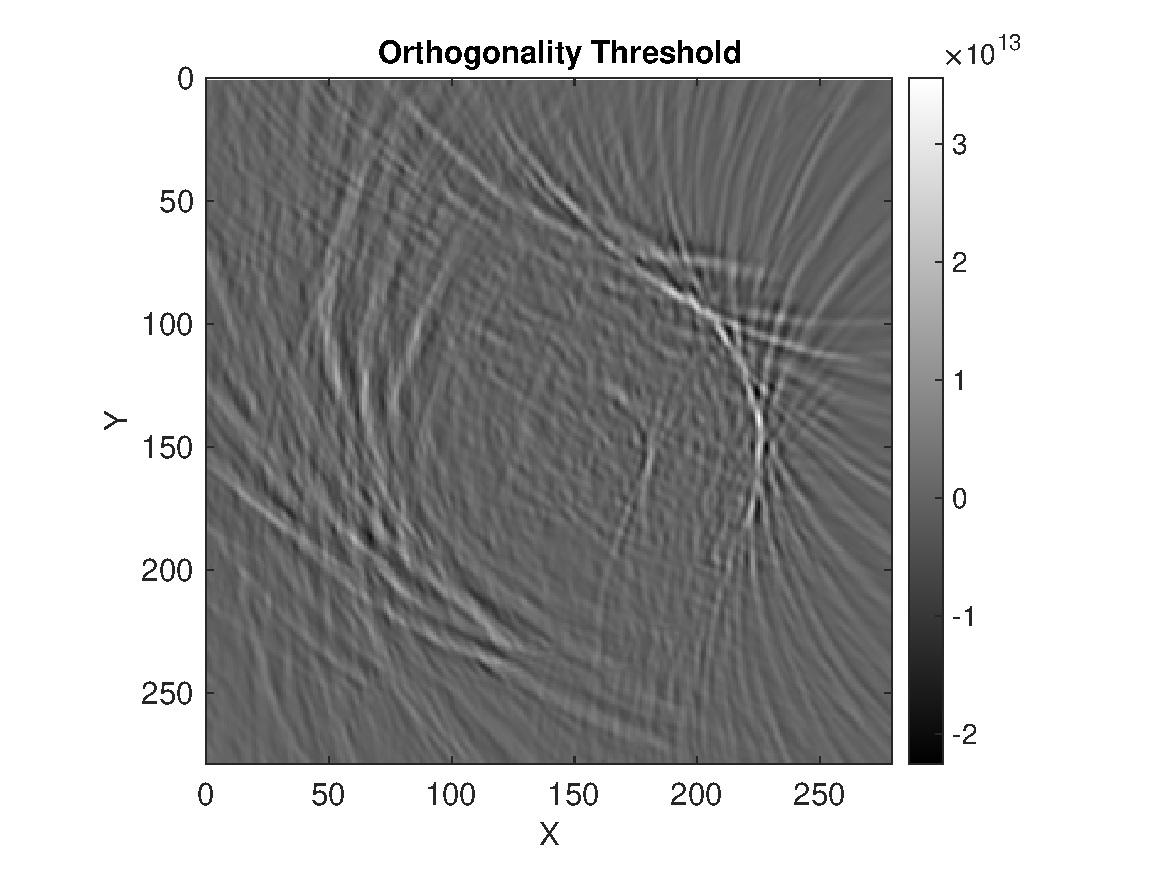
\includegraphics[width=1.12\linewidth,right]{Graphics/Results/Diff_angle_sort_orthogonality/diff_ortho_bubble_slice_166_3_ortho.eps}
         \caption{Orthogonality threshold method.}
         \label{fig:res:slice_diff_bubble_ortho_image_ortho}
     \end{subfigure}
     \hfill
     \begin{subfigure}[b]{0.49\textwidth}
         \centering
         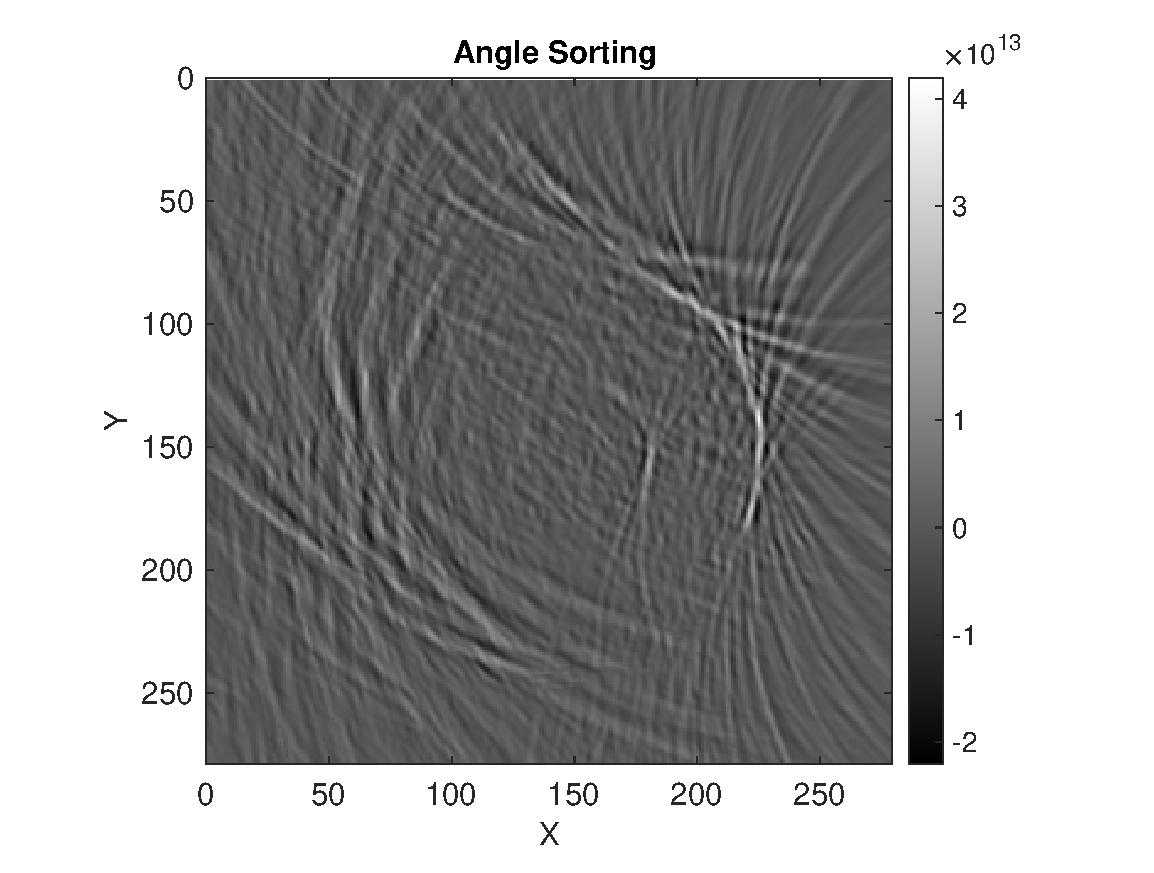
\includegraphics[width=1.12\textwidth,right]{Graphics/Results/Diff_angle_sort_orthogonality/diff_ortho_bubble_slice_166_3_sort.eps}
         \caption{Angle sorting method.}
         \label{fig:res:slice_diff_bubble_ortho_imagebubble}
     \end{subfigure}
        \caption{Side by side comparison of the resulting images for both methods. 25 directional vectors in total were used. The images are shown for the 3\textsuperscript{rd} directional vector and the 166\textsuperscript{th} slice in the z-dimension.}
        \label{fig:res:slice_diff_bubble_ortho_image}
\end{figure}



Both methods yield a very similar image. In both cases the outline of the 



Figure \ref{fig:res:slice_diff_bubble_ortho_imagebubble} on the right shows a slightly higher contrast than its counterpart on the left. The reason for that is that the Angle Sorting method of section \ref{chap:angle_sorting} assigns every available \ac{ascan} to a directional vector whereas the Orthogonality Threshold method discards every \ac{ascan} for which the comparison vector lay between the cones. This is not an inherent characteristic of this method. For this thesis it was implemented in a way that the decision regions all are the same size and overlap as little as possible. This leads to a assignment of directional index with as little ambiguity as possible. The equal and non-overlapping decisions regions that are schematically shown in Figure \ref{decision_arbitrary_circular} lead to a consistent quality of the assignment with the same decision criteria for each directional vector. In the example of the Angle Sorting method the decision criteria resulted in different acceptance angles depending on whether the comparison vector towards the tip of the pentagon or more towards the bisector between two directional vectors. In these cases the quality of the assignment can vary depending on what geometrical boundaries the Angle Sorting method has to follow.  In theory the Orthogonality Threshold method could use overlapping decision regions which regard every \ac{ascan} and thus, the resulting image should have the same contrast as the image from the Angle Sorting method.

\bigskip

In the following image the two methods are compared for one voxel in each of the 25 volumes in the 4\textsuperscript{th} dimension. This representation is similar to the one in Figure \ref{fig:res:5th_dim_over_4th_result} where the 5\textsuperscript{th} dimension was plotted over the 4\textsuperscript{th} dimension. Since there is not 5\textsuperscript{th} dimension this time only the 4\textsuperscript{th} dimension is plotted. For this representation there is also the analogy of the Rubik's cubes in figure \ref{4D_rubics}. Instead of the four Rubik's Cubes we now have 25 and for each of those cubes the voxel value at the the coordinates $[150\, , \, 150\, , \, 166]$ is displayed. For the directional vectors 22 to 25 no or only very few values are shown. The reason for that again is that those directional vectors are pointing out of the aperture and there are no receivers that could detect or emit a signal. 


\begin{figure}[H]
     \centering
     \begin{subfigure}[b]{0.85\textwidth}
         \centering
        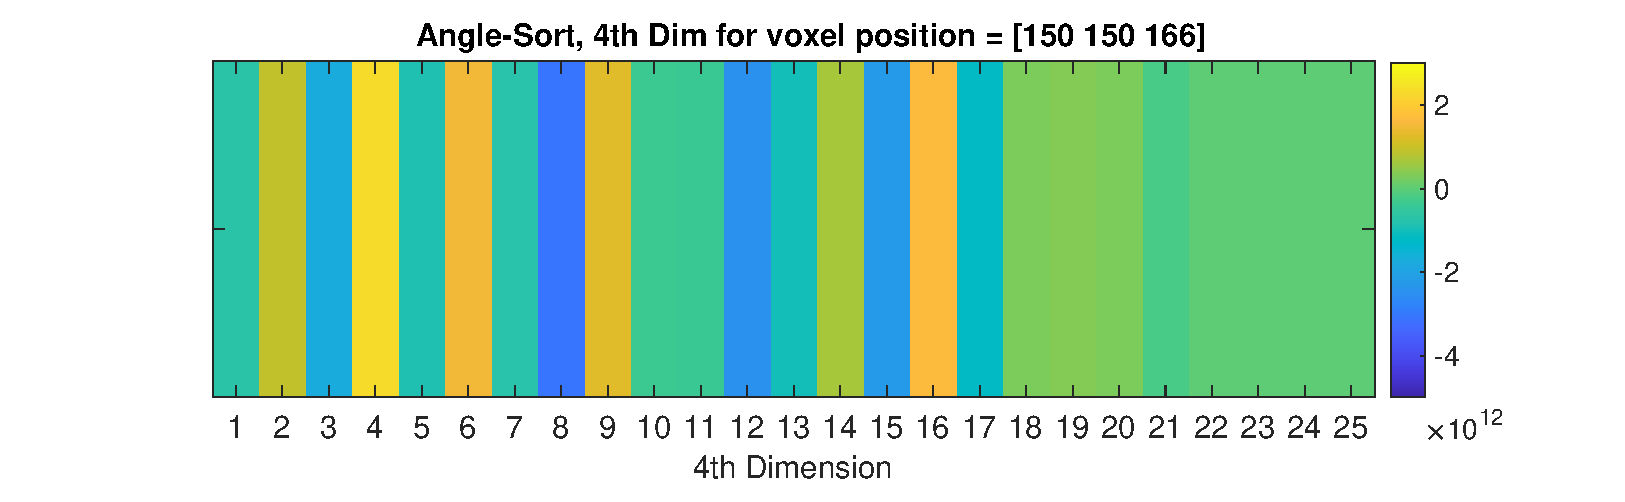
\includegraphics[width=1.12\linewidth,right]{Graphics/Results/Diff_angle_sort_orthogonality/diff_ortho_bubble_25dim_150150150_ortho.eps}
         \caption{Orthogonality threshold method.}
         \label{fig:res:25_voxel_values_diff_bubble_ortho_image_ortho}
     \end{subfigure}
     \hfill
     \begin{subfigure}[b]{0.85\textwidth}
         \centering
         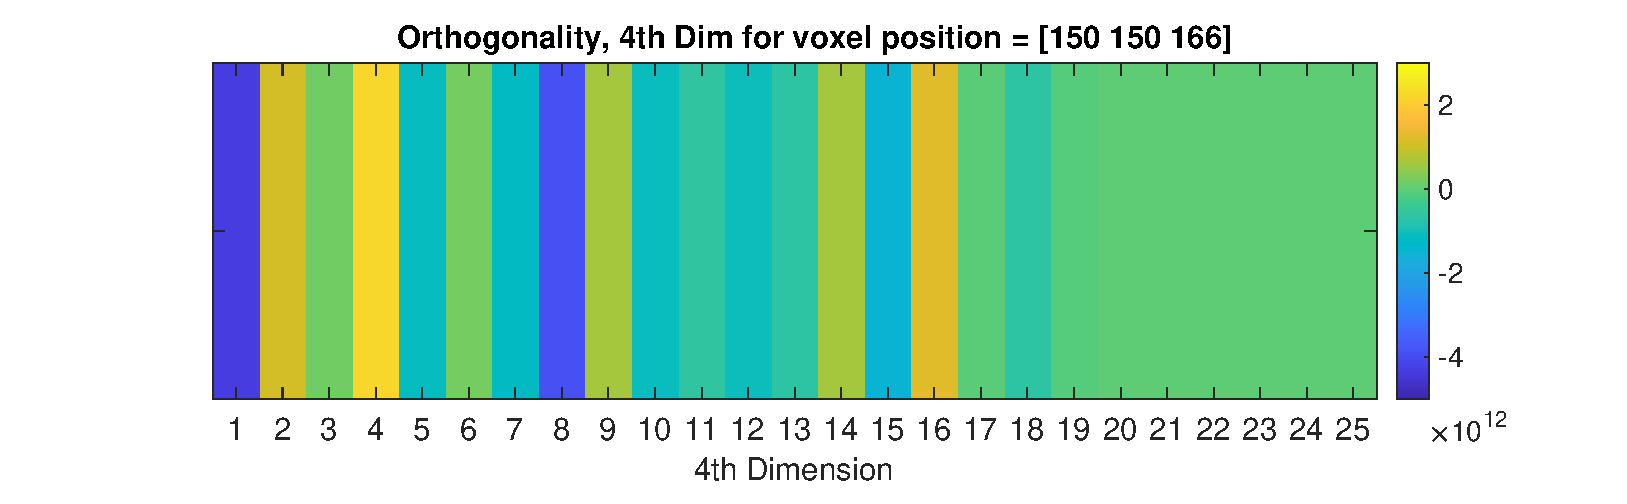
\includegraphics[width=1.12\textwidth,right]{Graphics/Results/Diff_angle_sort_orthogonality/diff_ortho_bubble_25dim_150150150_sort.eps}
         \caption{Angle sorting method.}
         \label{fig:res:25_voxel_values_diff_bubble_ortho_image_bubble}
     \end{subfigure}
        \caption{Comparison of each voxel value for each of the 25 directional vectors.}
        \label{fig:res:25_voxel_values_diff_bubble_ortho_image}
\end{figure}

The overall structure of array of voxel values for the both methods looks similar. Still, there are some differences. For example for the 1st directional vector. The voxel value for the Orthogonality Threshold method was $-4.3171 \times 10^{12}$  where as the voxel value for the angle sorting method was $-7.1738\times10^{11}$ so with the angle sorting value being approximately six times higher. For the comparison of the other voxels Figure \ref{fig:Voxel_value_25} shows each voxel value for the total of 25 directional vectors. The red line shows the voxel values which where yielded by the Orthogonality Threshold approach. The blue graph belongs to the Angle Sorting method. In most points the blue line lays above the red line. This corresponds to the assumption that the Orthogonality Threshold method does not consider every \ac{ascan} and therefore this method yields images with an overall lower contrast. In some cases the lines are congruent, in some they differ completely.  




\begin{figure}[H]
    \centering
    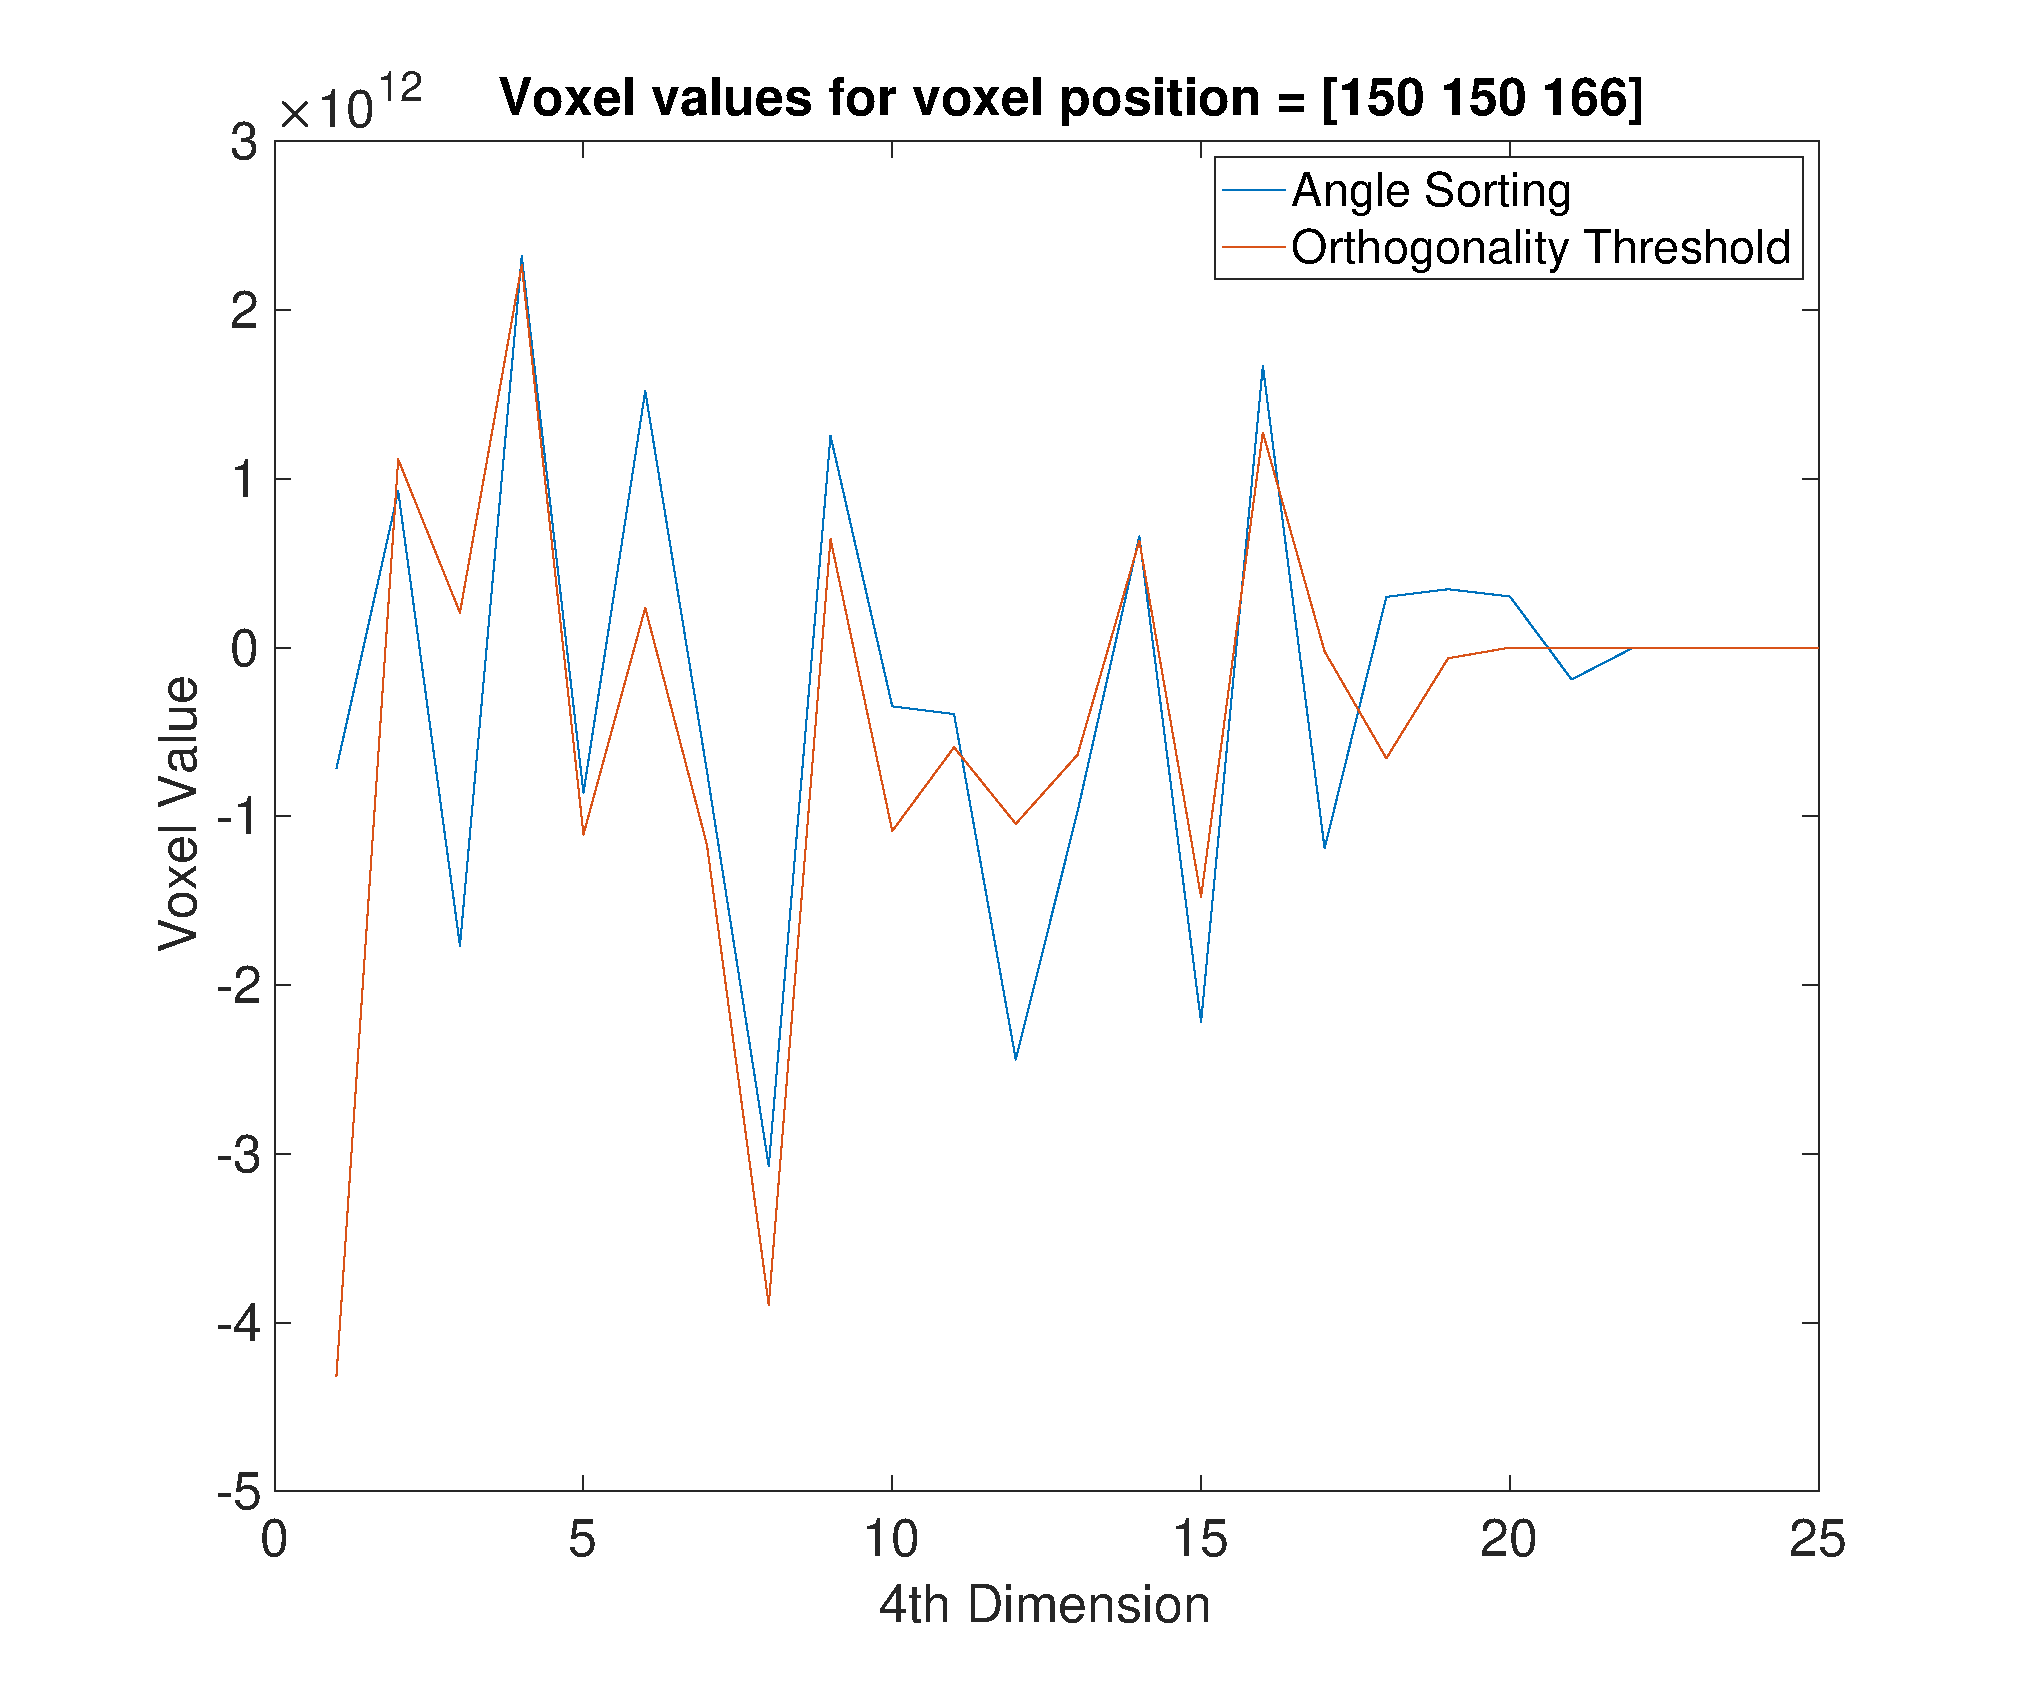
\includegraphics[width=0.82\linewidth]{Graphics/Results/Diff_angle_sort_orthogonality/diff_ortho_bubble_voxelvalues_150150166_sort.eps}
    \caption{Each voxel value of Figure \ref{fig:res:25_voxel_values_diff_bubble_ortho_image} as diagram. The blue graph belongs to the Angle Sorting Method and the red graph to the Orthogonality Threshold. }
    \label{fig:Voxel_value_25}
\end{figure}


To make an assessment about how big the influence of the reduced contrast of the Orthogonality Frequency method really is the reconstructed 4D images are both reduced to a 3D image. For each of the 25 sub-volumes the same voxel position is considered. This leads to 25 voxel values for one particular voxel in each volume. The mean of those 25 voxel values is calculated and written back into the coordinates of the particular voxel. This is repeated for every voxel there is. The final images are shown in the following Figure:


\begin{figure}[H]
     \centering
     \begin{subfigure}[b]{0.49\textwidth}
         \centering
         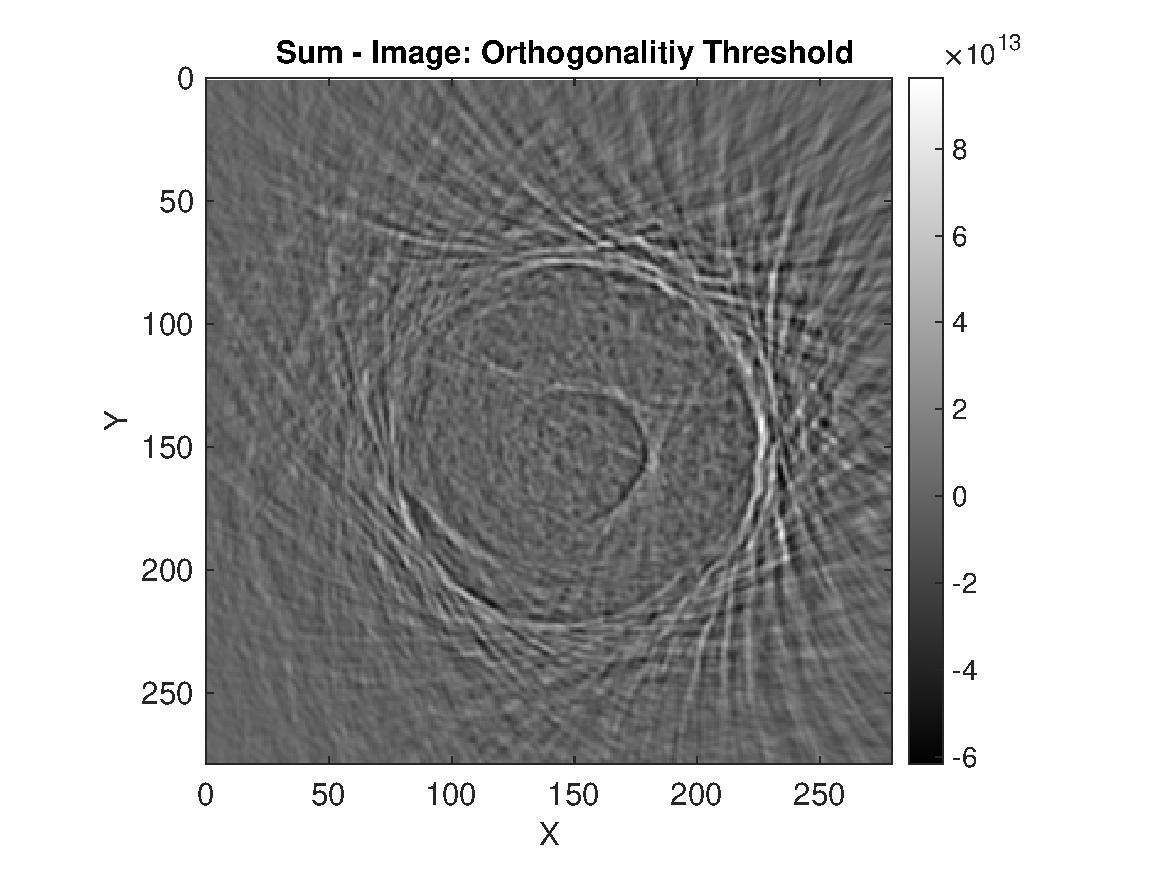
\includegraphics[width=1.12\linewidth]{Graphics/Results/Diff_angle_sort_orthogonality/diff_ortho_bubble_sumImmage_ortho.eps}
         \caption{Orthogonality Threshold method.}
         \label{fig:res:summareized_bubble_ortho_image_ortho}
     \end{subfigure}
     \hfill
     \begin{subfigure}[b]{0.49\textwidth}
         \centering
         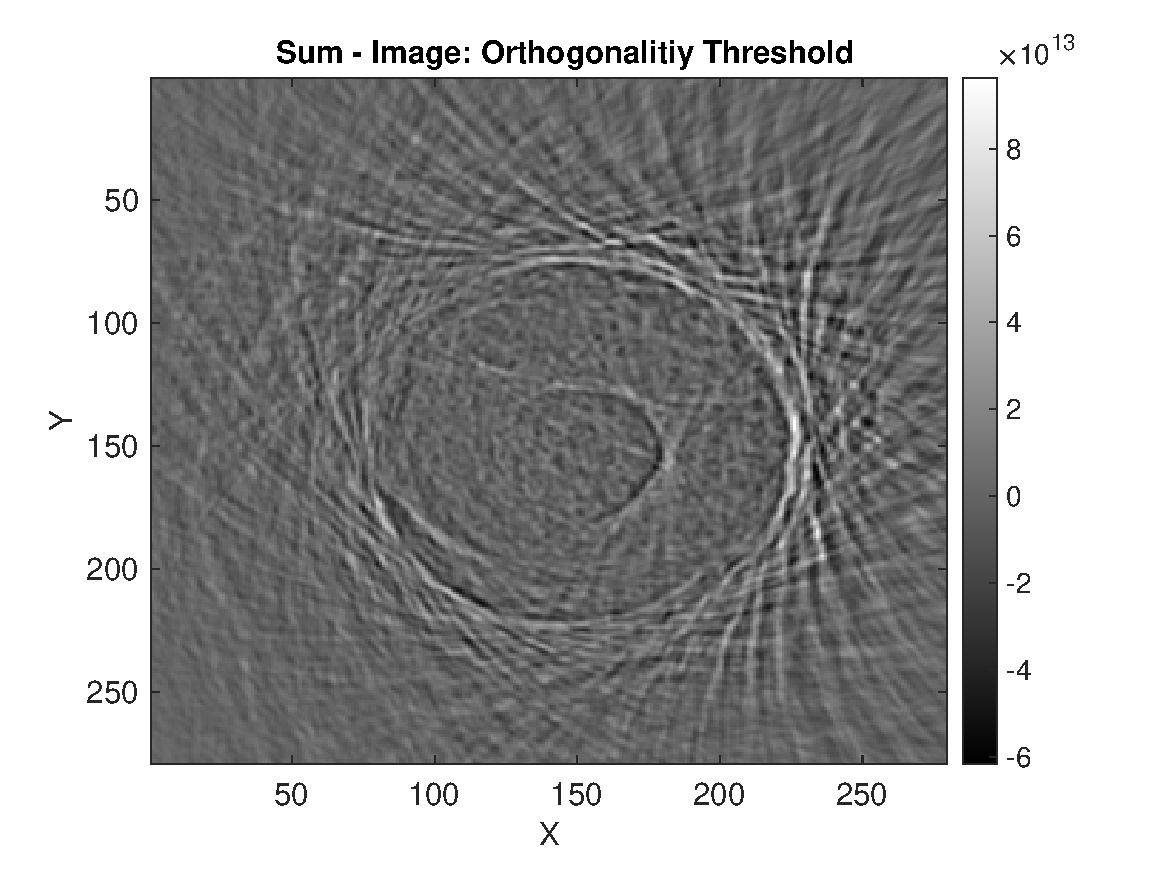
\includegraphics[width=1.12\textwidth]{Graphics/Results/Diff_angle_sort_orthogonality/diff_ortho_bubble_sumImmage_sort.eps}
         \caption{Angle Sorting method.}
         \label{fig:res:summareized_bubble_ortho_image_bubble}
     \end{subfigure}
        \caption{Summarised image where the 4D image was reduced to a 3D image. }
        \label{fig:res:summareized_bubble_ortho_image}
\end{figure}

Again the 166\textsuperscript{th} slice in the z-direction is shown. In comparison to Figure \ref{fig:res:slice_diff_bubble_ortho_image} the olive in the middle of the volume become much more prominent. In the image of only one directional vector the olive in Figure \ref{fig:res:slice_diff_bubble_ortho_imagebubble} showed a high intensity of sound waves in the top right corner of the olive. This become more prominent in the gelatin block as well. With the summation of all the images this information is lost. The images of both images contain enough information to make out the gelatin block with the olive in the middle. The difference between the two summarised images from Figure \ref{fig:res:summareized_bubble_ortho_image} is shown next:

\begin{figure}[H]
    \centering
    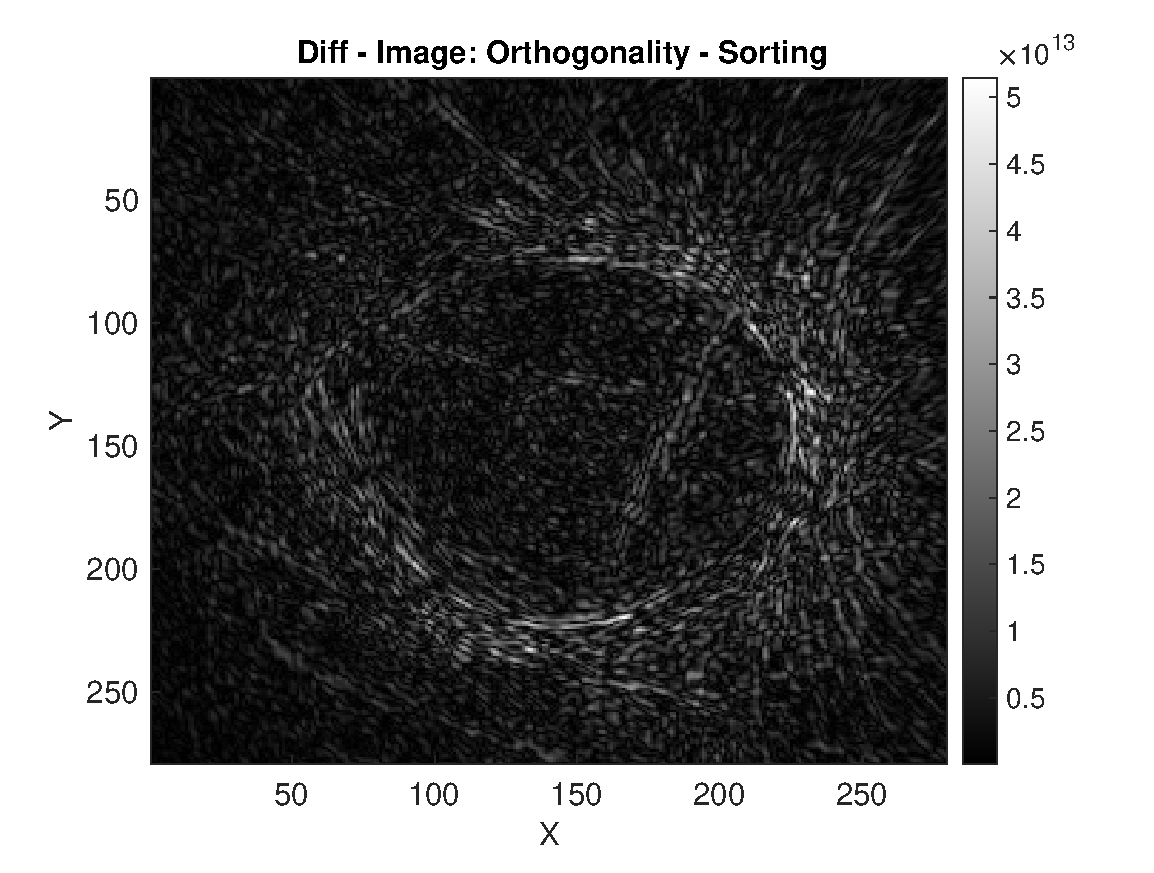
\includegraphics[width=0.82\linewidth]{Graphics/Results/Diff_angle_sort_orthogonality/diff_ortho_bubble_diffimage.eps}
    \caption{Absolute value of the difference between the summarised image of the Orthogonality Method and the Angle Sorting method. }
    \label{fig:diff_image}
\end{figure}

The biggest differences can be observed on the outer boundary of the gelatin block with a high density of reflections. The inside of the olive and the rest of the measurement volume are less influenced by the new method. Therefore, both methods yield an image with a high enough contrast so that the details are observable.





\section{Performance of the directional dimension assignment methods}
\label{performance_index_ident}

In Section \ref{sec:index_ident} two main approaches were presented for the assignment of the directional vector index to each \ac{ascan}. In this chapter the results of the performance evaluation of the angle sorting approach from section \ref{chap:angle_sorting} and the threshold orthogonality from section \ref{chap:ortho_threshold} are shown. 

For the performance analysis the general structure of the reconstruction from Figure \ref{Basic_Algo_Angle_ident} is adapted. To speed up the process, the 5\textsuperscript{th} dimension is kept constant during the execution. This leads to a four dimensional image instead of a five dimensional. For the evaluation a script was written which calls the reconstruction function with an increasing amount of directional vectors. For each choice of the number of directional vectors the four dimensional image is reconstructed in whole. The procedure is repeated for the angle sorting approach and the new orthogonality approach separately.

The following calculations were performed on two \acp{gpu} with a reconstruction volume of 279x279x233 voxels. Furthermore, only the first block of 30235 \acp{ascan} were used during the reconstruction to speed up the process. The four dimensional case was considered and therefore only the comparison vector from the voxel to the receiver was used. No results besides the profiling report were saved to minimise the influence of hard drive operations during the performance evaluation. The execution time includes all initialisation steps of the reconstruction algorithm as well as generation of directional vectors. The calculation of the threshold orthogonality (in case of the application of the orthogonality threshold method) is also considered by these results. The first reconstruction was started for 14 directional vectors and the last ended at 126. The current implementation allows to generate and abitrary set of directional vectors starting at 14. Sets with fewer directional vectors than 14 were generated with the platonic solid approach. For the performance evaluation it was necessary to increase the number of directional vectors arbitrarily and the evaluation starts with 14 input vectors.

The following three figures shows the comparison of the computation time of the different techniques for the index identification introduced in section \ref{sec:index_ident}. The results for the sorting algorithm are presented in blue where as the approach with the orthogonality threshold is shown in red.

\begin{figure}[H]
    \centering
    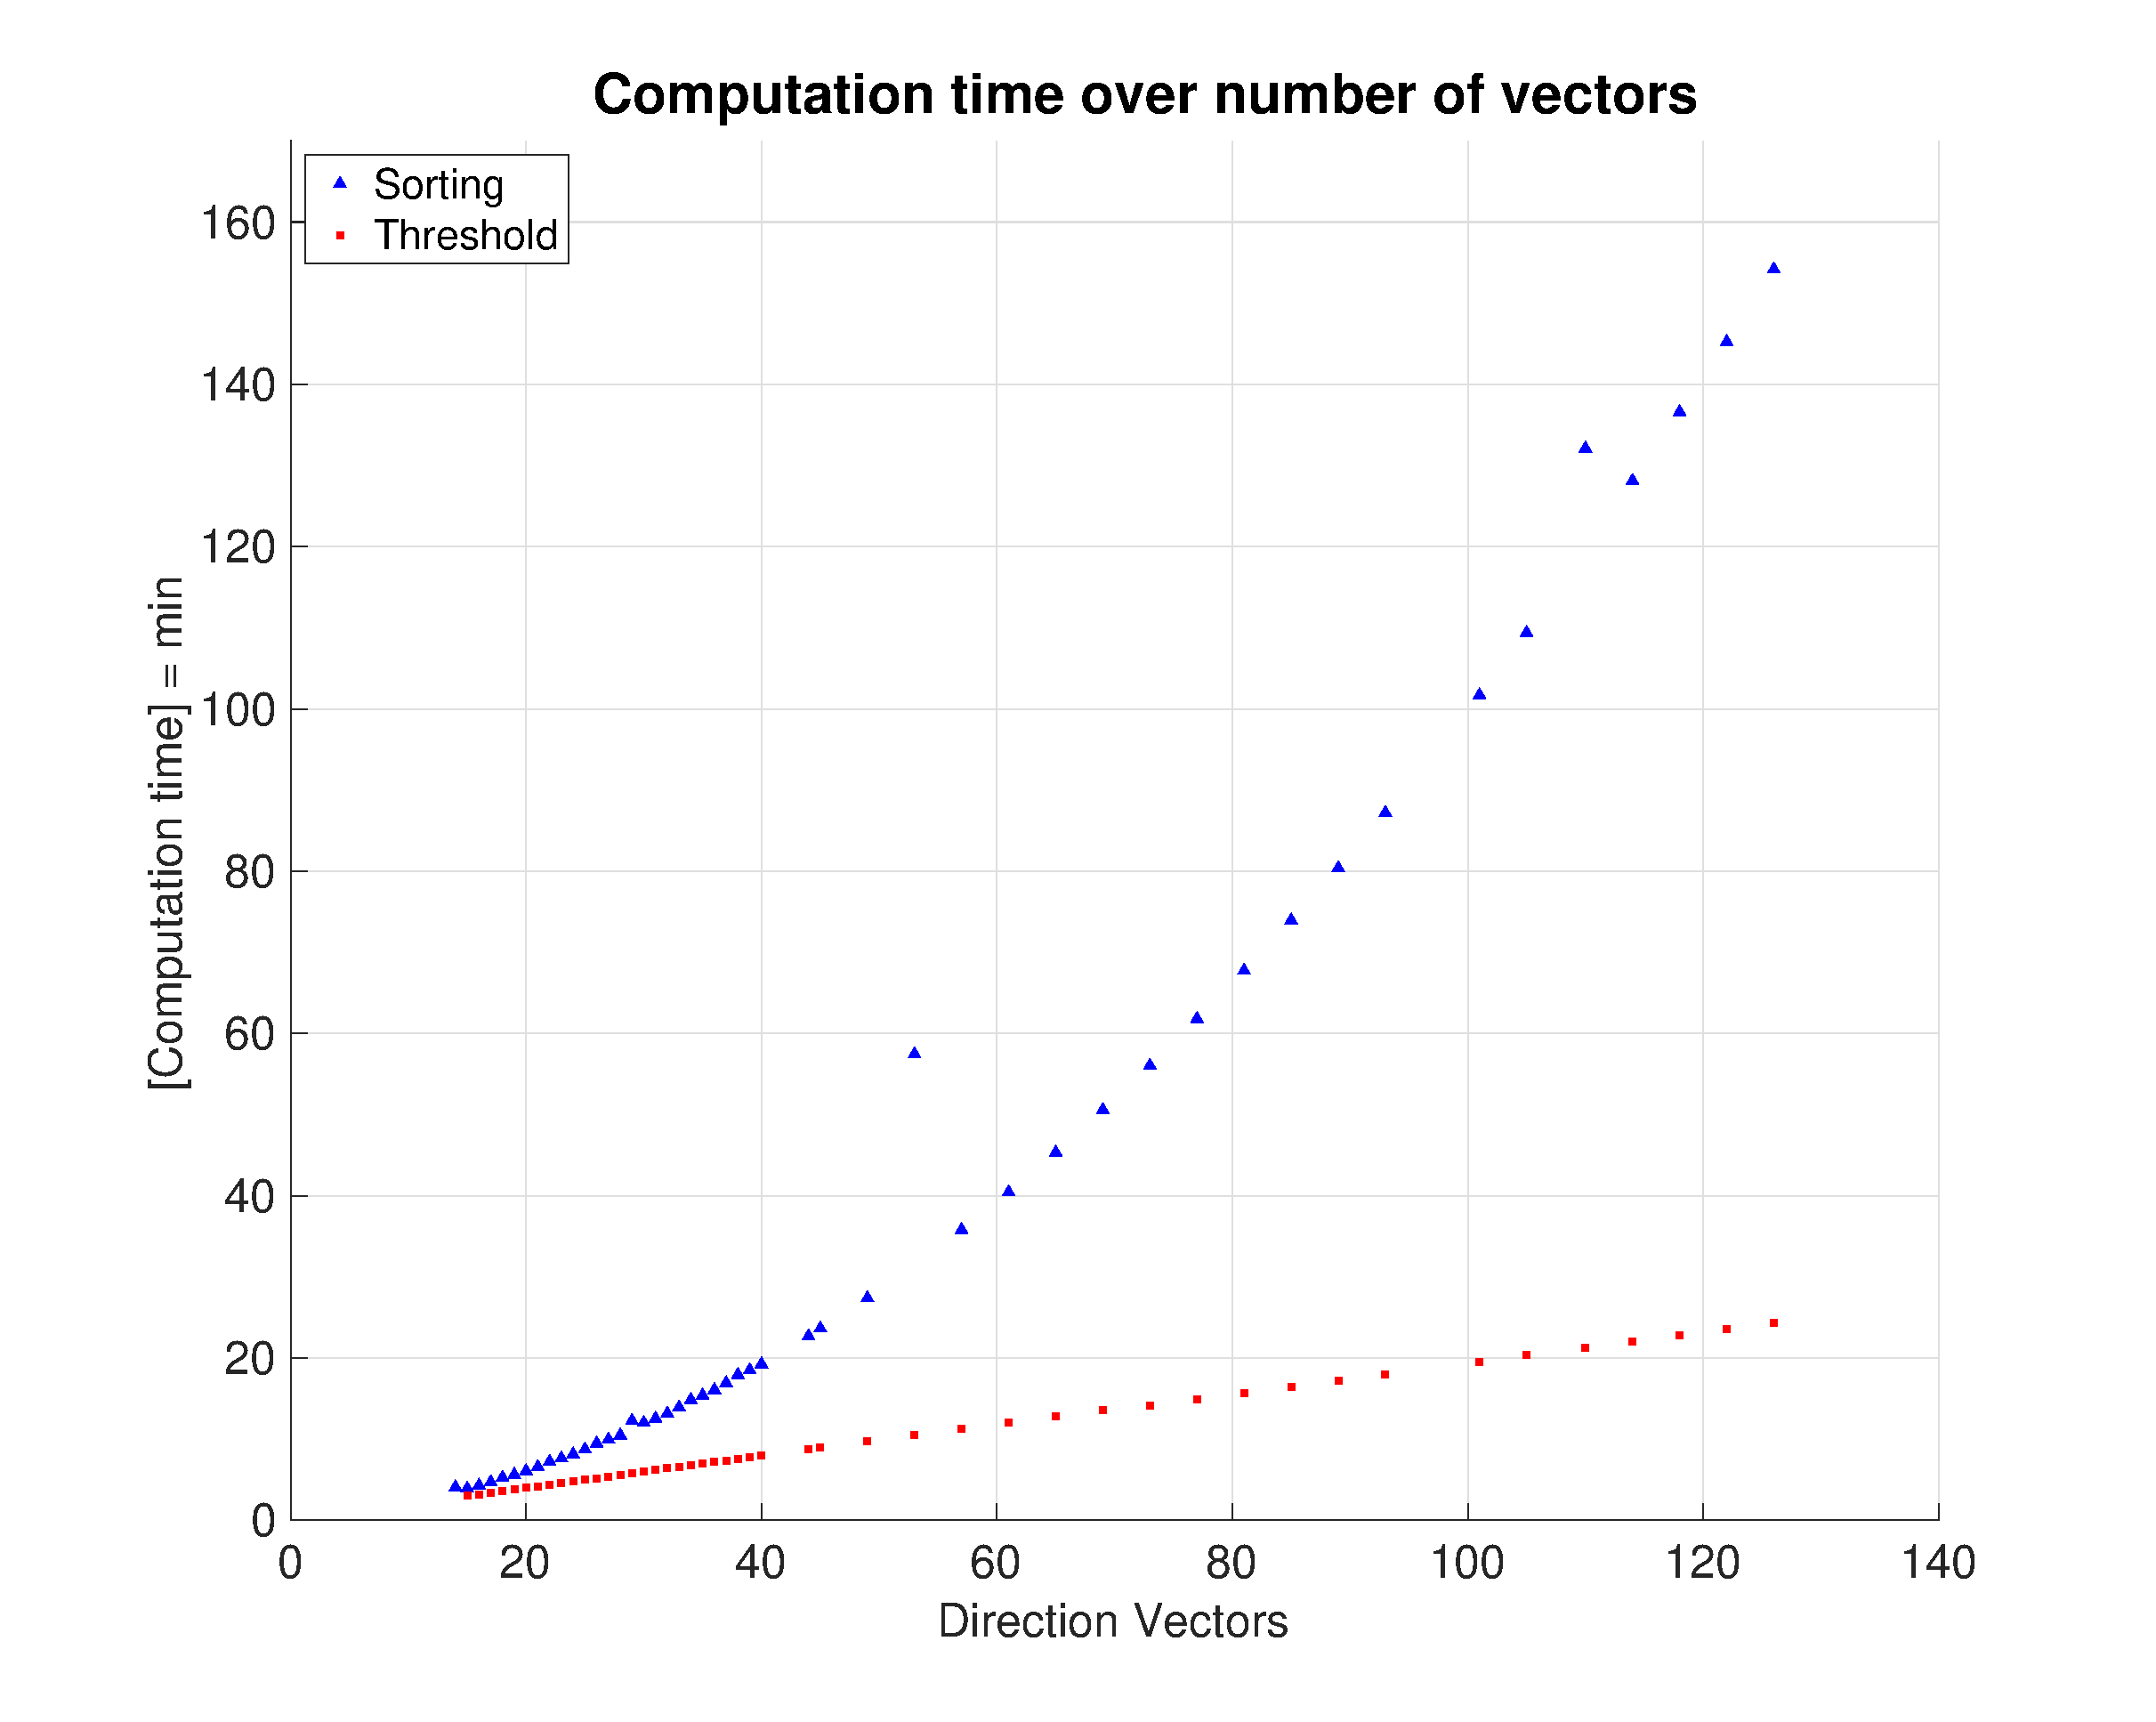
\includegraphics[width=1\linewidth]{Graphics/Results/complete_computation_time_over_numer_vec.eps}
    \caption{Total time of computation given in minutes for 30325 \acp{ascan} and for all loops over the directional vectors. The red markers represent the execution time for the orthogonality threshold method. The blue markers belong to the angle sorting algorithm.}
    \label{fig:Complete_computation_all_vecs}
\end{figure}

The blue triangle markers in Figure \ref{fig:Complete_computation_all_vecs} represent the execution time for the angle sorting algorithm. The horizontal distances between the succeeding markers is associated with the attempt to decrease the overall length of the experiment. For shorter execution times (up to 20 minutes per call) for both algorithms the amount of directional vectors were increased one by one after each iteration. The following steps were increased by four input vectors per iteration.

For a small number of directional vectors the execution time of the angle sorting algorithm and the orthogonality threshold are relatively close, both taking approximately three minutes to compute. With increasing number of directional vectors the application of the angle sorting algorithm leads to a longer sorting loop. This can be seen in the exponential growth of the execution time for the implementation of the angle sorting method. In contrast the implementation of the orthogonality threshold method shows a linear behaviour when the number of directional vectors is increased. For the final 126 directional vectors the sorting algorithm takes $154 \min$ whereas the orthogonality method takes $24,3 \min$ to finish, thus being $10,5$ times higher than the faster orthogonality method. For 45 directional vectors the reconstruction with the angle sorting method takes $23,6 \min$ and thus approximately as long as the orthogonality method takes with 126 directional vectors.

The execution times of each iteration and number of directional vectors include a significant amount of overhead, as it was mentioned further above. Since the overhead is expected to be constant for every execution of the reconstruction algorithm. Regardless of the overhead these results still show the considerable influence of the assigning algorithm on the overall performance.

During the performance evaluation certain iterations took an unusual amount of time to finish and led to some outliers in the computation time for the sorting algorithm. Those were non-reproducible for the particular number of directional vectors for when they occurred but were kept in the graph for reasons of consistency. One possible explanation might be the accidental use of the same  \acp{gpu} by another process or other occurrences that might have led to the simultaneous occupation of servers resource and thus a decreased performance of the reconstruction algorithm since multiple people have access to it.


\begin{figure}[H]
    \centering
    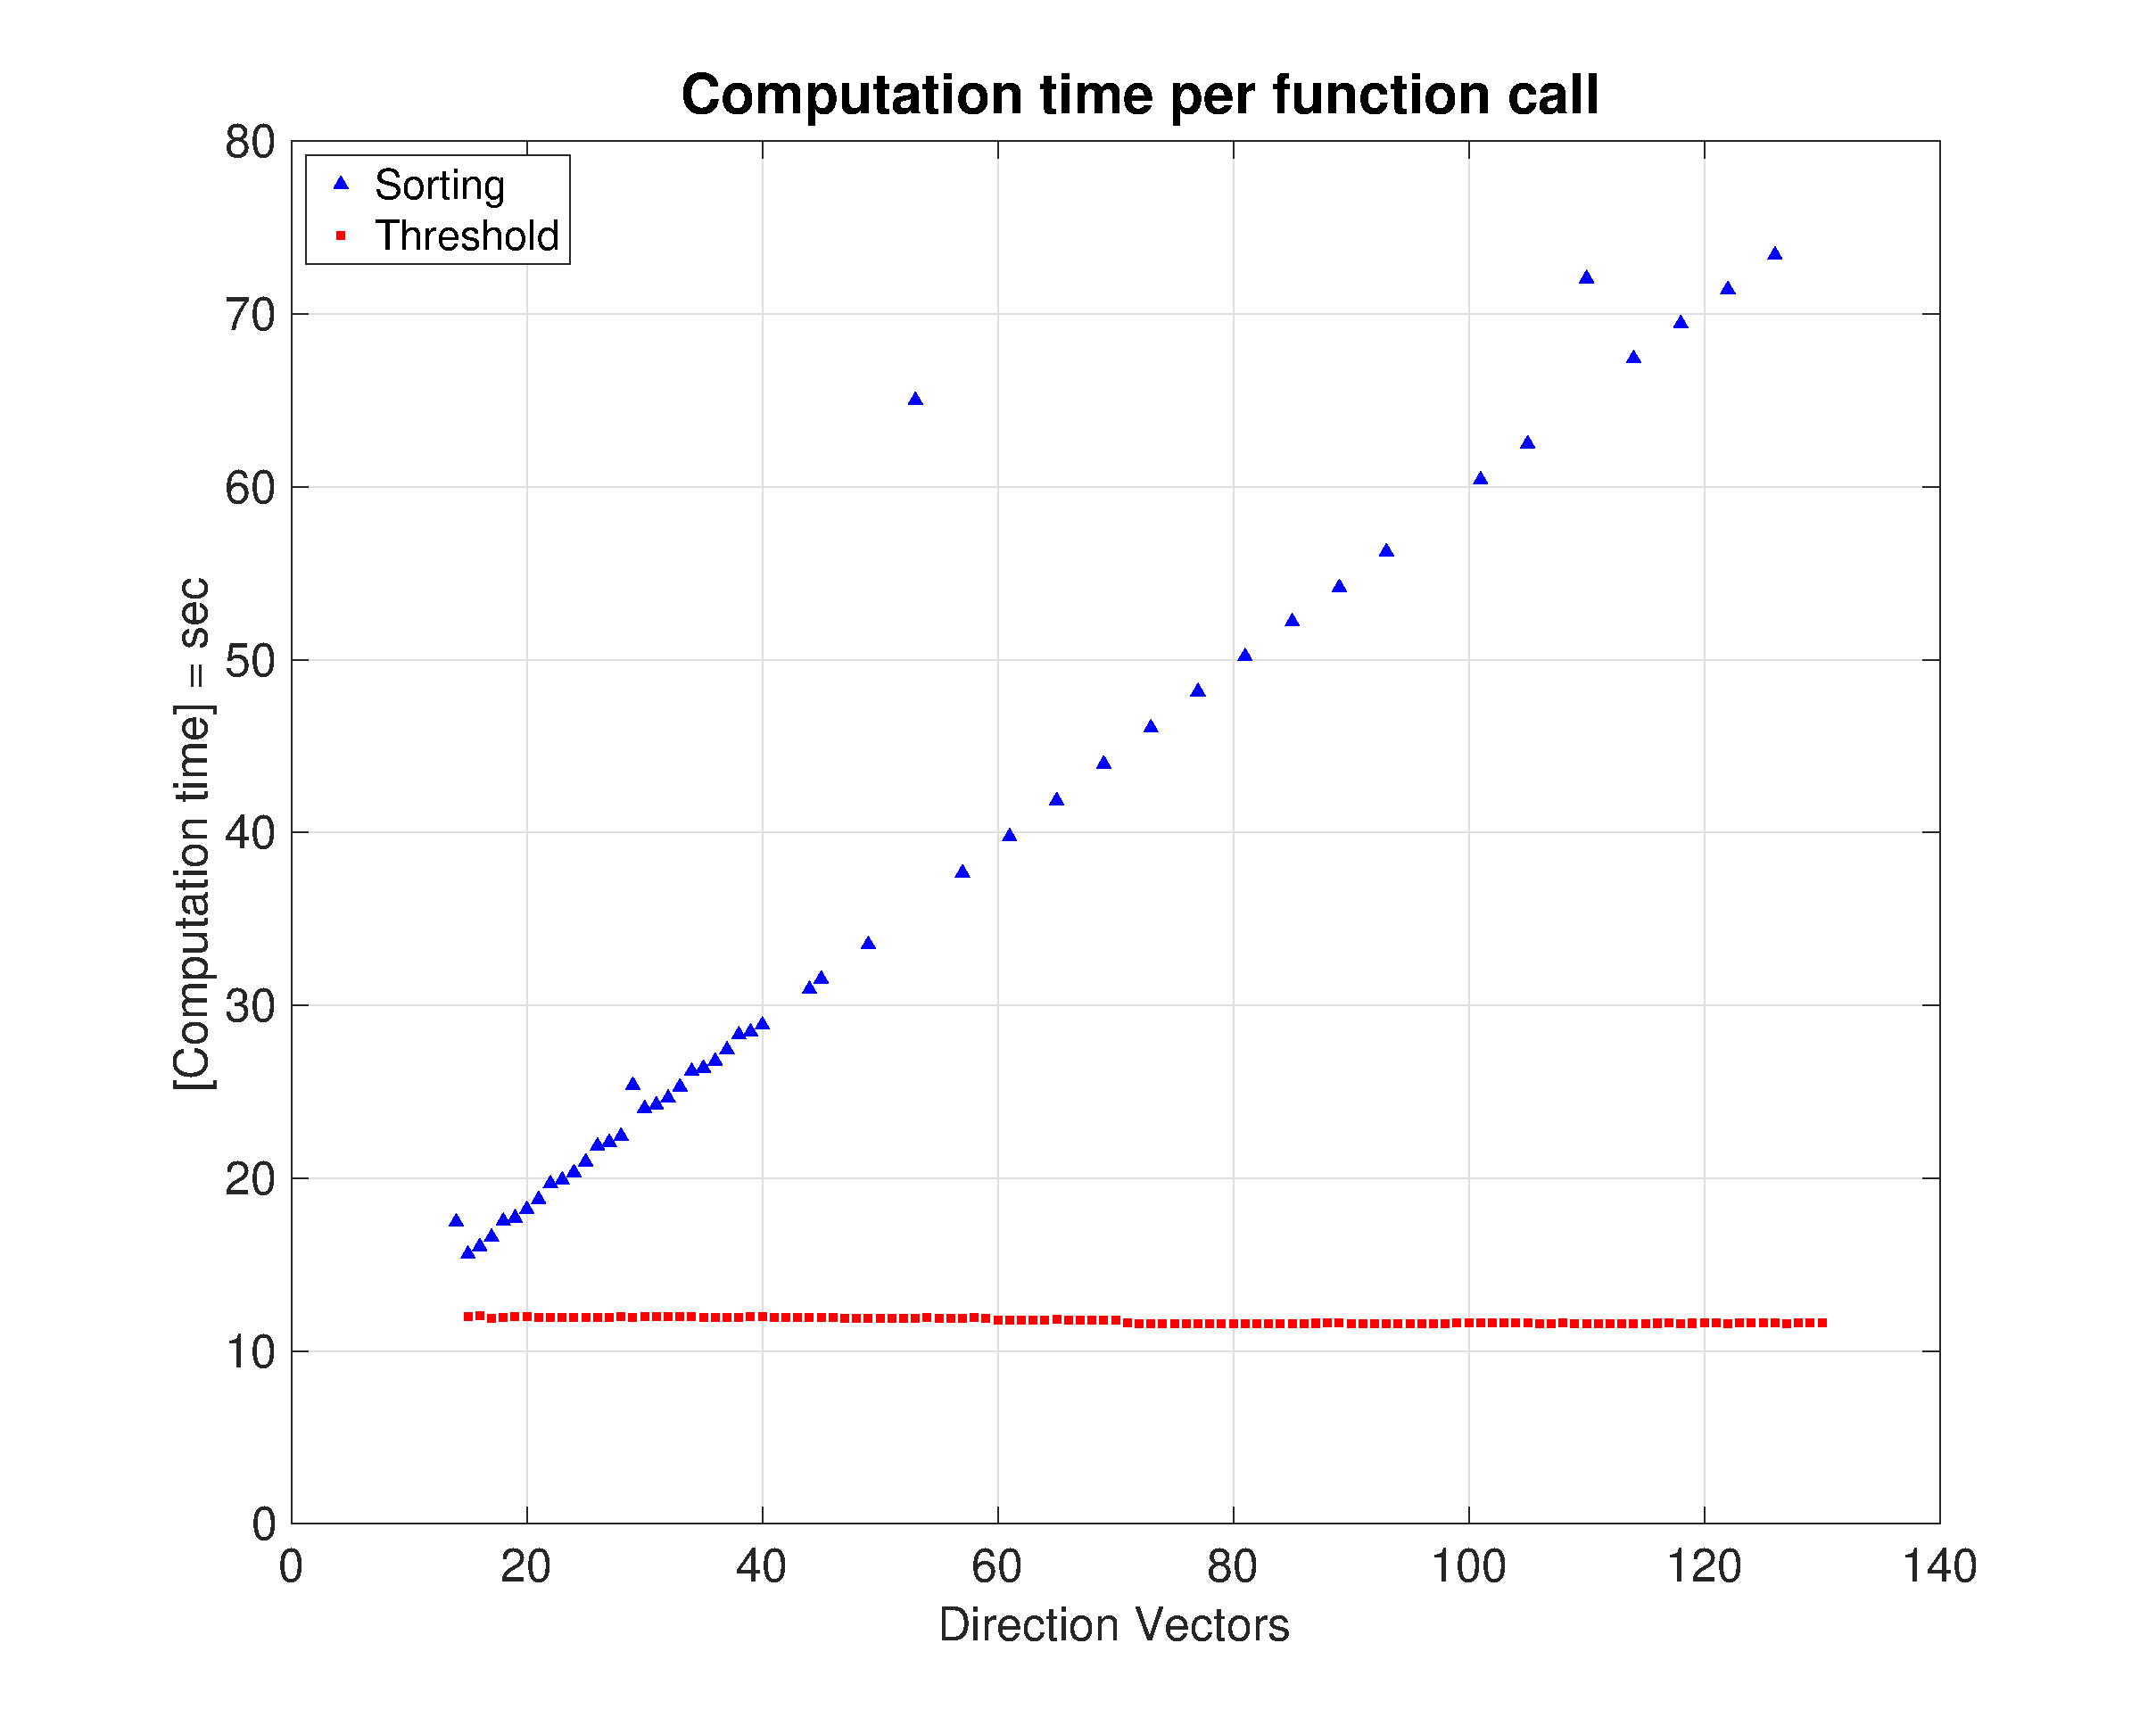
\includegraphics[width=1.08\textwidth]{Graphics/Results/computation_time_per_mexcall.eps}
    \caption{The computation time of each individual function call in $\sec$. The complete execution time was divided by the   }
    \label{fig:computation_per_mex}
\end{figure}

In Figure \ref{fig:computation_per_mex} the execution time for only one iteration of the reconstruction is shown. The complete computation time was divided by the number of input directional vectors to approximate the execution duration for only one function call. The resulting plot shows that the execution time for the orthogonality threshold method is rather constant for an increasing number of directional vectors. In contrast the execution time for each function call with the implementation of the sorting algorithm takes an increasing amount of time to finish. The outliers in the set of blue markers are visible again in this plot. The red markers for the threshold method seem to have a step at about 70 input vectors. The reason for that most likely is the different time of day when the executions were started. They were not done consecutively but sometimes had to be restarted at a later point. This also was the case for the performance analysis for the threshold method. Beginning with 70 input directional vectors the profiling script was restarted the day after. The reason for the small difference in execution time again might be found in the shared resources on the server and the non-constant load during the calculations. 



\begin{figure}[H]
    \centering
    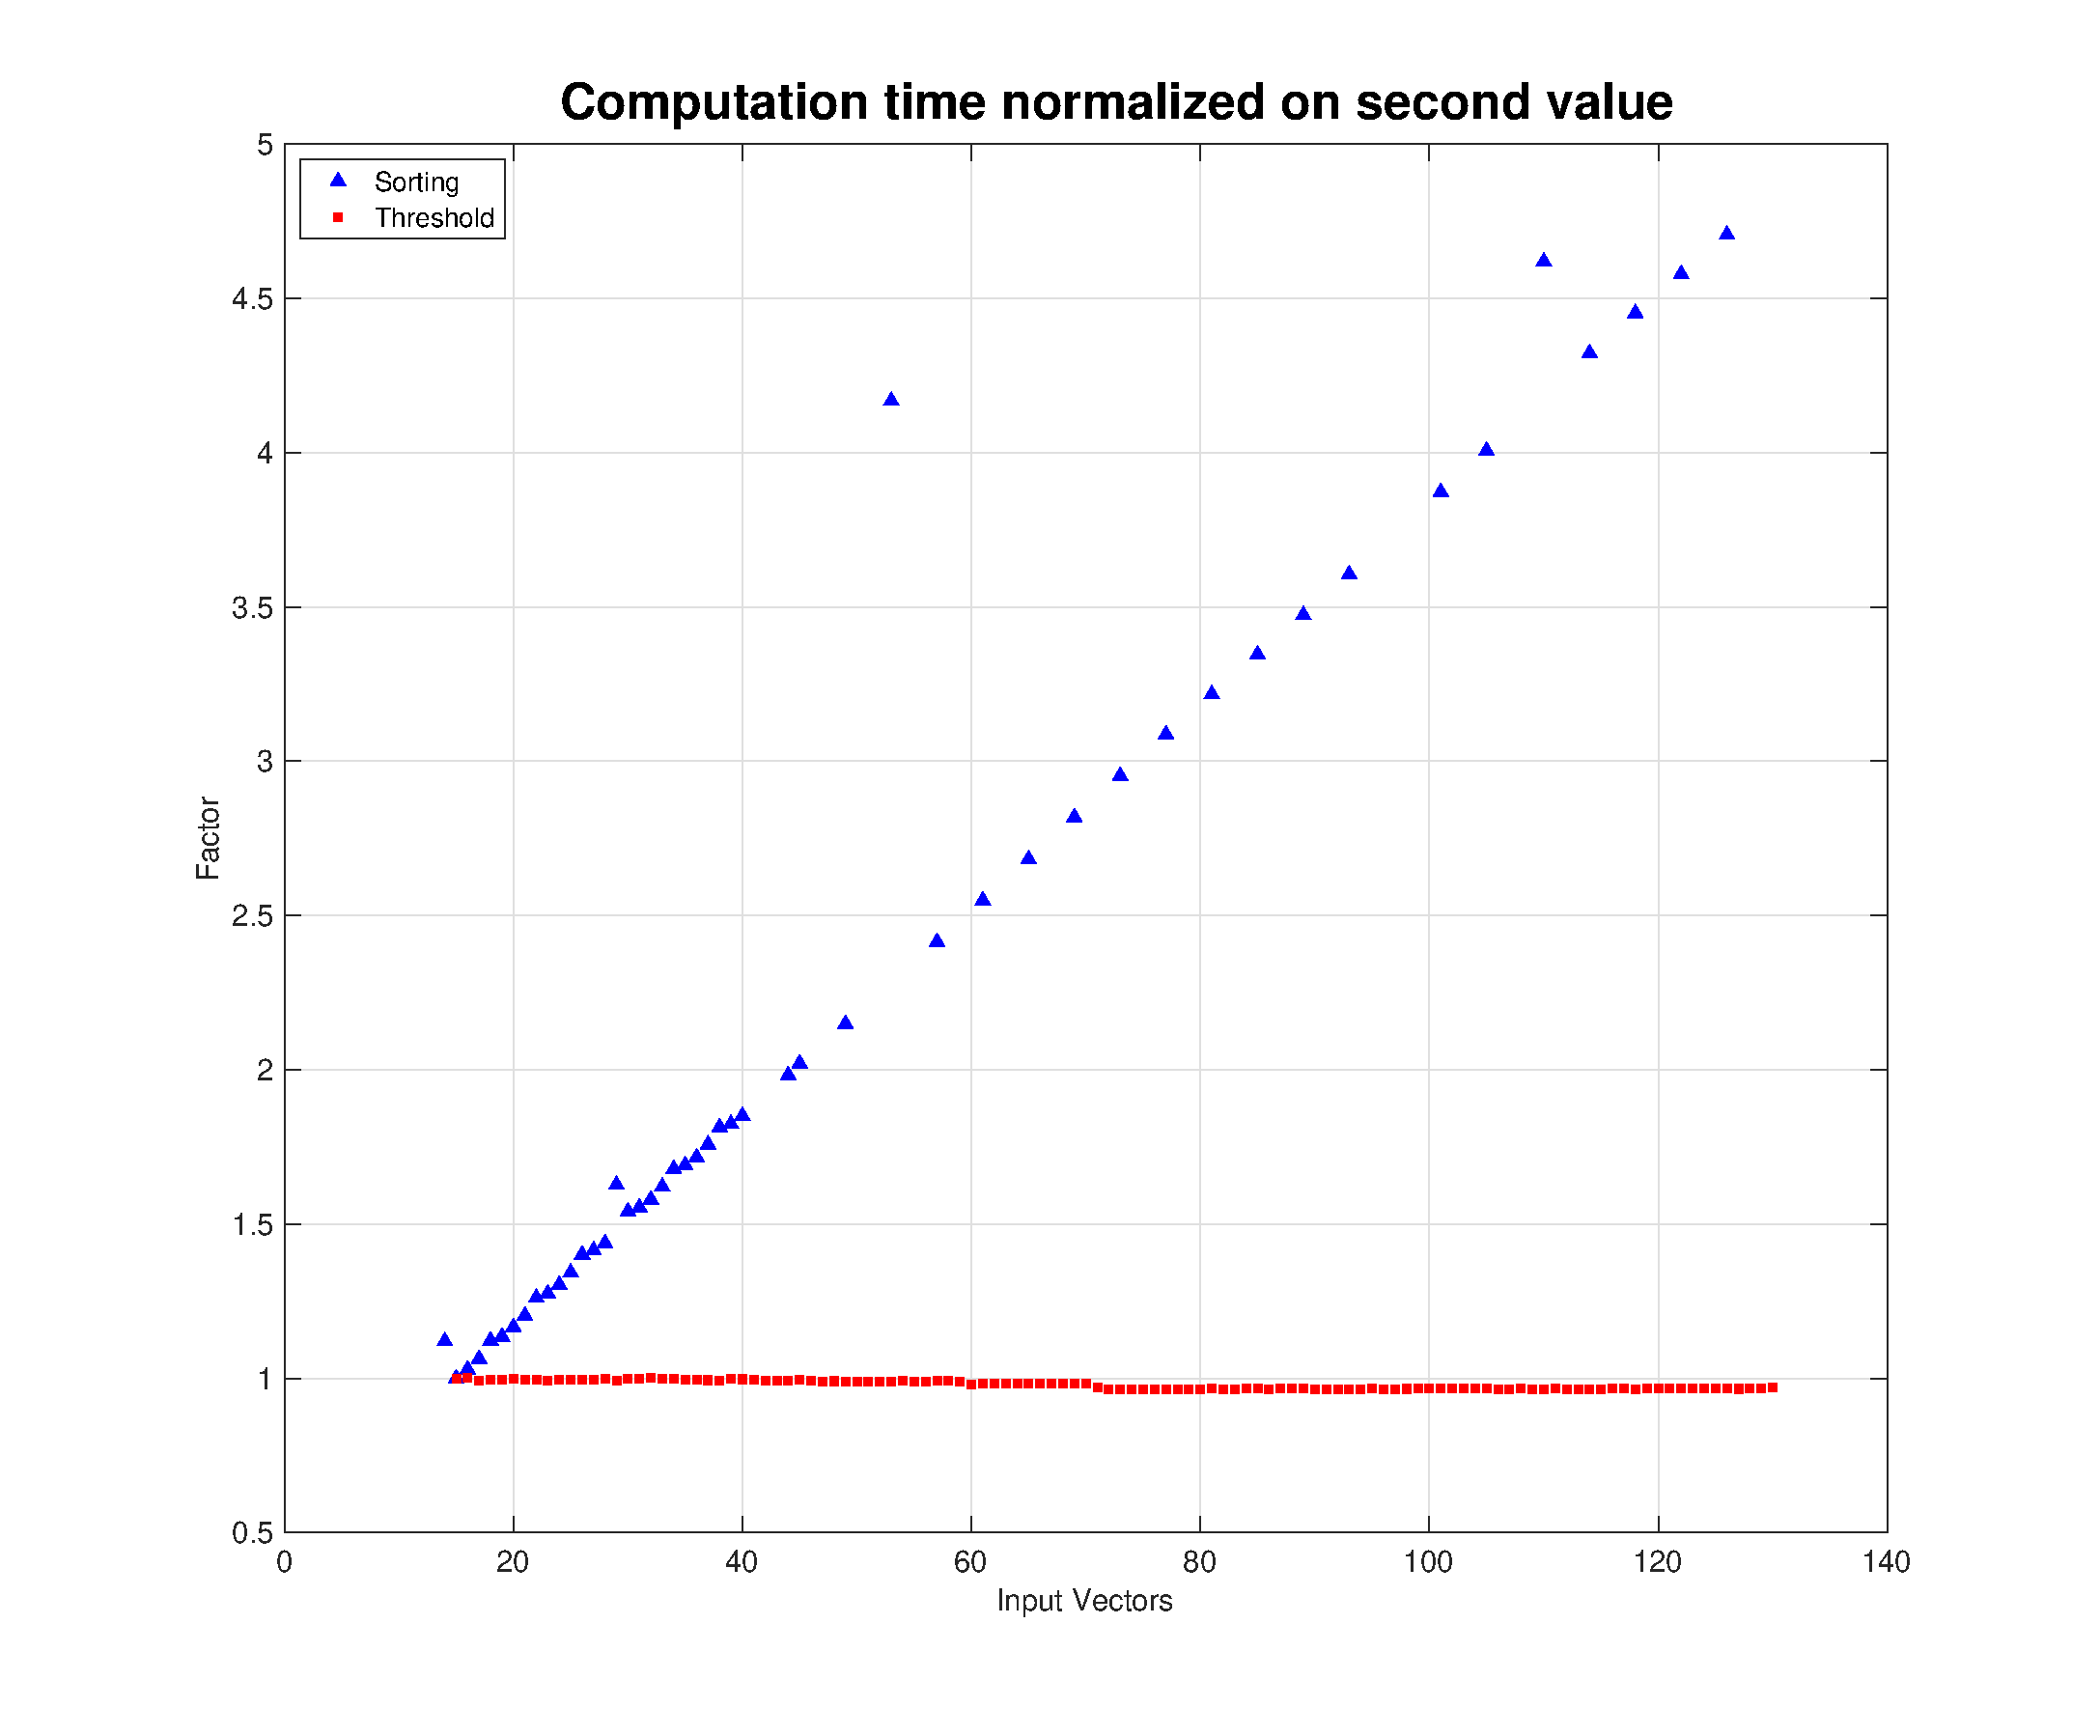
\includegraphics[width=1.08\textwidth]{Graphics/Results/computation_normlaized_2nd_value.eps}
    \caption{The computation time of each individual function call was normalised on the 2nd value of both methods.}
    \label{fig:computation_normlaized_2nd}
\end{figure}

To quantify the differences in performance between both approaches in Figure \ref{fig:computation_normlaized_2nd} the execution times for both methods were normalised on their respective second value. The second value was preferred over the first one since the first iteration always took a bit longer than the following one. A reason for that might be initial behaviour of the servers processing unit  e.g. the optimisation of the cache management at the beginning of the calculations. Nevertheless, in both cases the markers for 14 directional vectors begin at the factor 1 and increase over the following iterations with more input vectors. At least this is the case for the angle sorting method. The markers for the orthogonality threshold stay rather constant at 1 whereas the blue markers end up at a factor of $4.706$ for 126 input vectors. Here again the small step around the 70 input vectors arise from the different times of the start of the analysis.





\section{Evaluation of the distinguishability of different tissue textures}
\label{sec:res:eval_diff_tissue_type}


The following results all were created with the Orthogonality Threshold method from section \ref{chap:ortho_threshold} since this method has proven to be much more efficient (see section \ref{performance_index_ident}) as well as to yield an approximation of the results from the angle search method. The volume was restricted to minimise the computation time and Figure \ref{fig:res:reflec_image_olive_xyz} shows the location of the reconstructed volume. For these results 35 directional vectors were created with the arbitrary segmentation approach. Per \ac{tas} one sender and nine receivers were regarded. To reduce the computation time only four of the ten available aperture positions were included.  



In section \ref{fig:res:5th_dim_over_4th_result} the 5D-over-4D-representation of different voxels inside of the 5D data was introduced. This representation shall now be used to analyse the characteristics of different tissue types. The 5D-over-4D-representations for the three different test voxels is plotted in Figure \ref{fig:res:5D_4D_skin_pulp_compare}. 

In this image we see all the 4D-5D values for each of the sub-volumes of the reconstructed data. As a reminder: the 5\textsuperscript{th} dimension comprises directional information for the directional from the voxel to the emitters whereas the 4\textsuperscript{th} dimension contains the information for the voxel to the receiver. With that in mind it becomes clear that the directional vectors $30, 31, 32, 33, 34$ and $35$ are pointing out of the imaging aperture and neither any emitter nor any receiver is located in this directional. Therefore, neither of the three 5D-4D-representation does hold any directional information for those directional vectors.

\begin{figure}[H]
     \centering
     \begin{subfigure}[b]{0.69\textwidth}
         \centering
        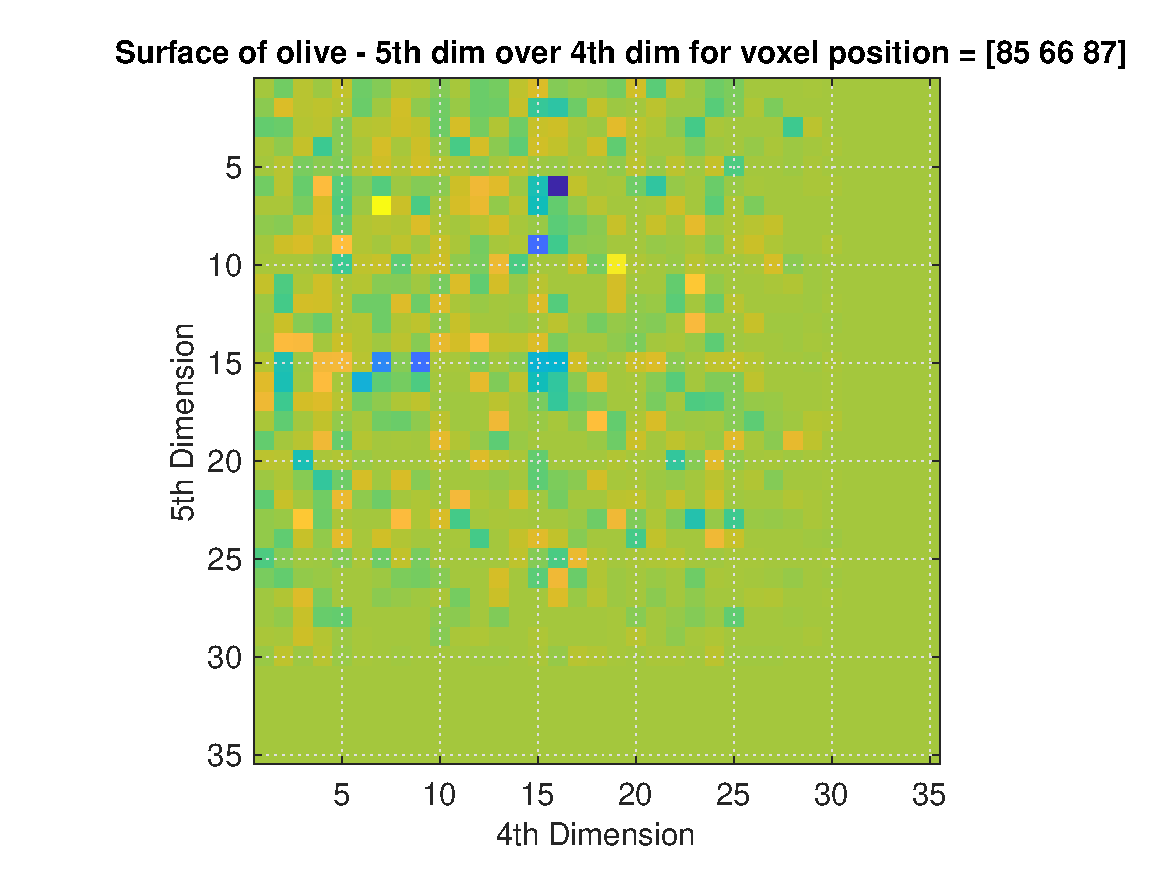
\includegraphics[width=0.9\linewidth]{Graphics/Results/skin_pulp_stone_5D_4D_Stone.eps}
         \caption{Olive. }
         \label{fig:res:5D_4D_skin_pulp_compare_stone}
     \end{subfigure}
     \hfill
     \begin{subfigure}[b]{0.69\textwidth}
         \centering
         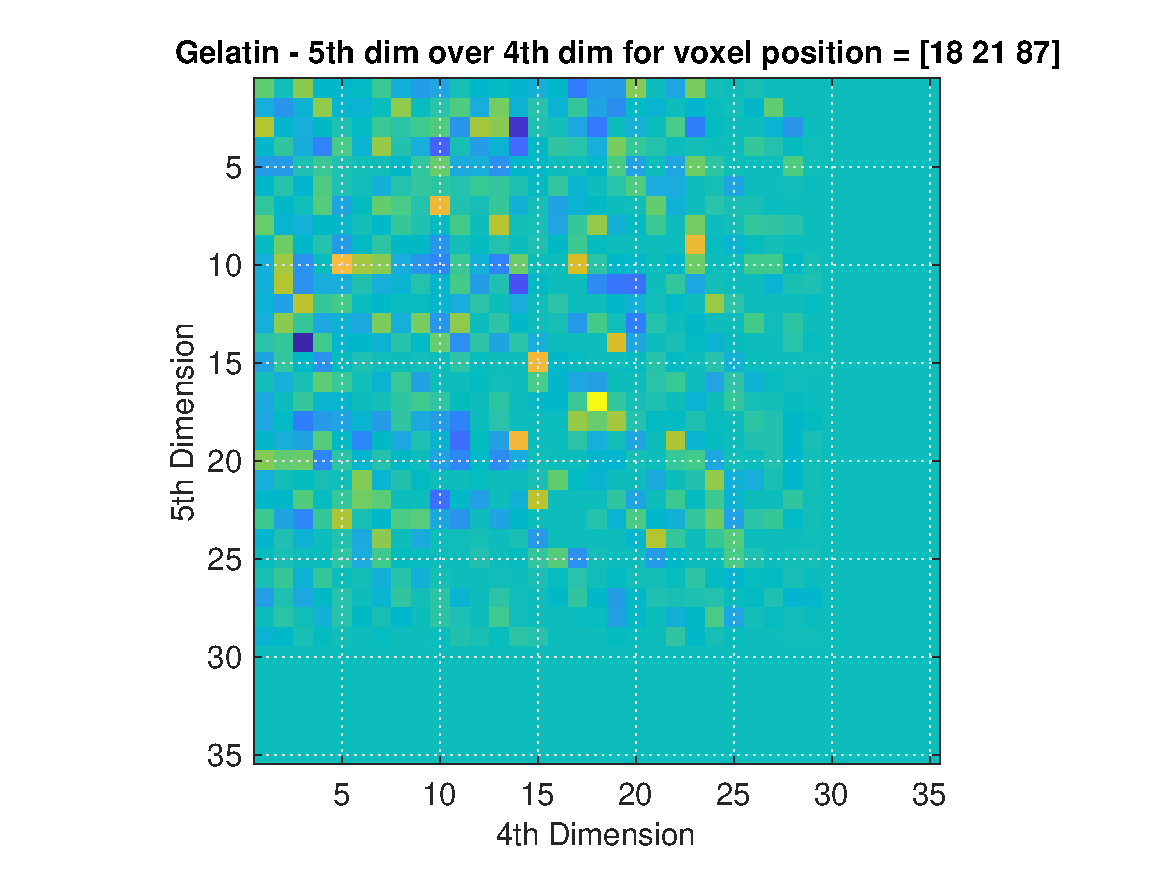
\includegraphics[width=0.9\textwidth]{Graphics/Results/skin_pulp_stone_5D_4D_Pulp.eps}
         \caption{Gelatin. }
         \label{fig:res:5D_4D_skin_pulp_compare_pulp}
     \end{subfigure}
          \hfill
     \begin{subfigure}[b]{0.69\textwidth}
         \centering
         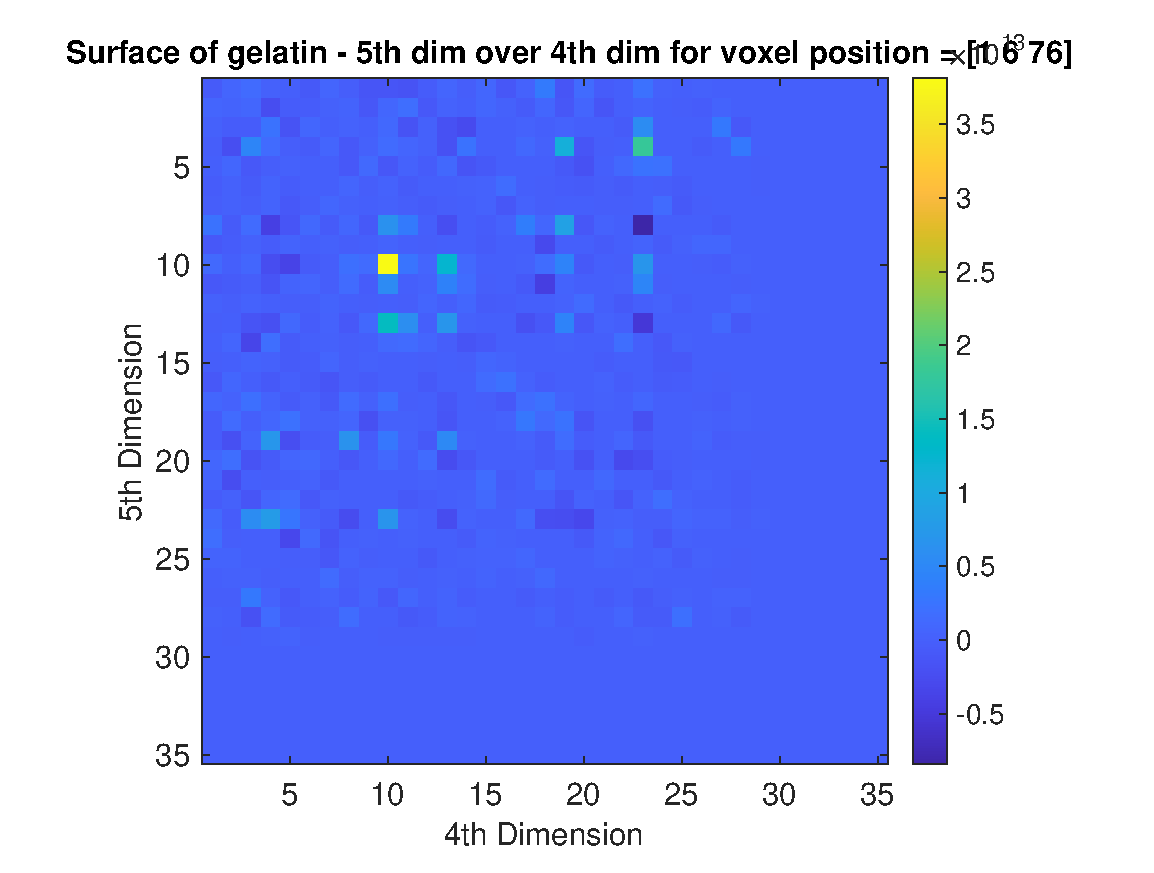
\includegraphics[width=0.9\textwidth]{Graphics/Results/skin_pulp_stone_5D_4D_Skin.eps}
         \caption{Surface of gelatin. }
         \label{fig:res:5D_4D_skin_pulp_compare_skin}
     \end{subfigure}
        \caption{ 5D-over-4D representation of three different voxels in the reconstructed image. It is assumed that the olive skin and the surface of the gelatin block both have a prevailing specular reflection characteristic whereas the gelatin and the pulp of the olive are assumed to have predominantly diffuse properties. }
        \label{fig:res:5D_4D_skin_pulp_compare}
\end{figure}

 




\medskip


In Figure \ref{fig:res:5D_4D_skin_pulp_compare_stone} we see the 5D-over-4D-representation for the voxel located at the \textbf{stone} of the olive. This plot can be used to make a first assertion about the tissue characteristics of the examined sample. The stone is assumed to have strong specular reflectivity properties since it has a hard and relatively even surface.
For the case of a specular reflection the angle of the incoming ultrasound wave has the same angle as the reflected sound wave as it was explained in section \ref{sig:flect_character}. The expected outcome for specular reflections would result in high values around the leading diagonal of the image where $4D = 5D$. In these cases the incoming sound wave was emitted from an emitter that lay in the same direction as the receiver that received that echo. In case of the 5D-over-4D-image of the stone there is one big value on the leading diagonal at the locations (6,6), (15,15) and (16,16). These values give the first clue about the specular parts of the reflection properties of the medium at the location of that pixel.
Apart from the high values on the leading diagonal there are some peaks at the location (16,6), (15,7), (15,9), (9,15). These points are symmetrically located to the main diagonal of the image which would support the assumption of the specular reflectivity of the object. In case of the pair (15,9) and (9,15) the receiver with the directional index 15 detects the signal which was emitted from an emitter with the directional index 9 and in addition to that the receiver 9 detects a signal from emitter 15 then the object can be assumed to be a specular scatterer. 

\medskip

In Figure \ref{fig:res:5D_4D_skin_pulp_compare_pulp} the 5D-over-4D-image for the \textbf{pulp} of the olive is shown. In comparison to the hard stone in the middle of the olive, the pulp is rather soft and has a homogeneous pattern. Therefore, this type of tissue is expected to have diffuse reflection properties. This can also be seen in the representation of the directional information. On the first glance the overall distribution of the values is much more unorganised. A symmetrical distribution of the values that was observed in Figure  \ref{fig:res:5D_4D_skin_pulp_compare_stone} is not given in the case of the pulp. This means that for a certain emitter direction many receiver in all kinds of directions detect the signal and vice versa that one receiver detects the pulse emitted by transducers that are not necessarily close to that receivers direction. On the leading diagonal of the image are only a few higher values. Two peaks are located at (10,10) and (15,15) which have a lower amplitude compared to the case of the stone, though. This leads to the conclusion that this type of tissue has some specular reflection properties but that they are not prevailing kind. The uneven distribution of values shows evidence of a diffuse scatterer. 

\medskip

For the last of the three test voxels the Figure \ref{fig:res:5D_4D_skin_pulp_compare} shows the characteristics for the \textbf{skin} of the olive. The even structure of the surface is assumed to reflect ultrasound waves in a specular manner. The 5D-over-4D-representation supports this assumption. A yellow peak value is located at (10,10) and therefore directly on the leading diagonal of the image. This means that the pulses that are emitted by the transducers located in the direction of the 10\textsuperscript{th} directional vector are also mainly detected at the receivers in the same direction. In addition to that a symmetrical distribution of the peaks can be observed. Directly around the yellow peak there are higher values located at (10,13) and (13,10) and a bit further away at (23,4) and (3,23). This again coincides with the observation that was made for the olive stone above and a prevailing specular reflectivity for that tissue sample can be assumed.




\section{Deviation-imaging \& Max-imaging}
\label{chap:devi_image}

Since the final image of the reconstruction contains 5 dimensions the results are not easy to display in an comprehensible way. One option of displaying all the data of the five dimensions in one 3D volume was shown in Figure \ref{fig:res:summareized_bubble_ortho_image}. In this case the voxel values were averaged along the 4\textsuperscript{th} dimension and the 5\textsuperscript{th} dimension. During this step also the directional information were averaged and therefore lost in the final image. This procedure results in a 3D image which is similar to the original \ac{usct}-images without any directional information.   

\bigskip

Another option for the representation of the data is the \textbf{Deviation image}. It can be calculated from the 5D-over-4D representations and results in a three dimensional image. The 5D-over-4D image resulted from plotting every voxel value for each sub-volume. This means that there are as many 5D-over-4D images containing the directional information of the image as there are voxels in the image. For each of these 5D-over-4D-images a standard deviation can be calculated. The results from section \ref{sec:res:eval_diff_tissue_type} showed a distinct pattern for tissue types with specular properties compared to tissue types with diffuse behaviour. For the specular kind there were some high peaks symmetrically distributed around the leading diagonal of the image whereas the diffuse tissue showed a more even distribution of value over the whole are of the image. With these observations in mind the standard deviation of a the 5D-over-4D characteristics for a specular scatterer should result in a higher value compared to the even distribution of the 5D-over-4D plot for the diffuse case. In the following Figure the Deviation image is shown next to the summarised 5D->3D image of the data set.


\begin{figure}[H]
     \centering
     \begin{subfigure}[b]{0.47\textwidth}
         \centering
        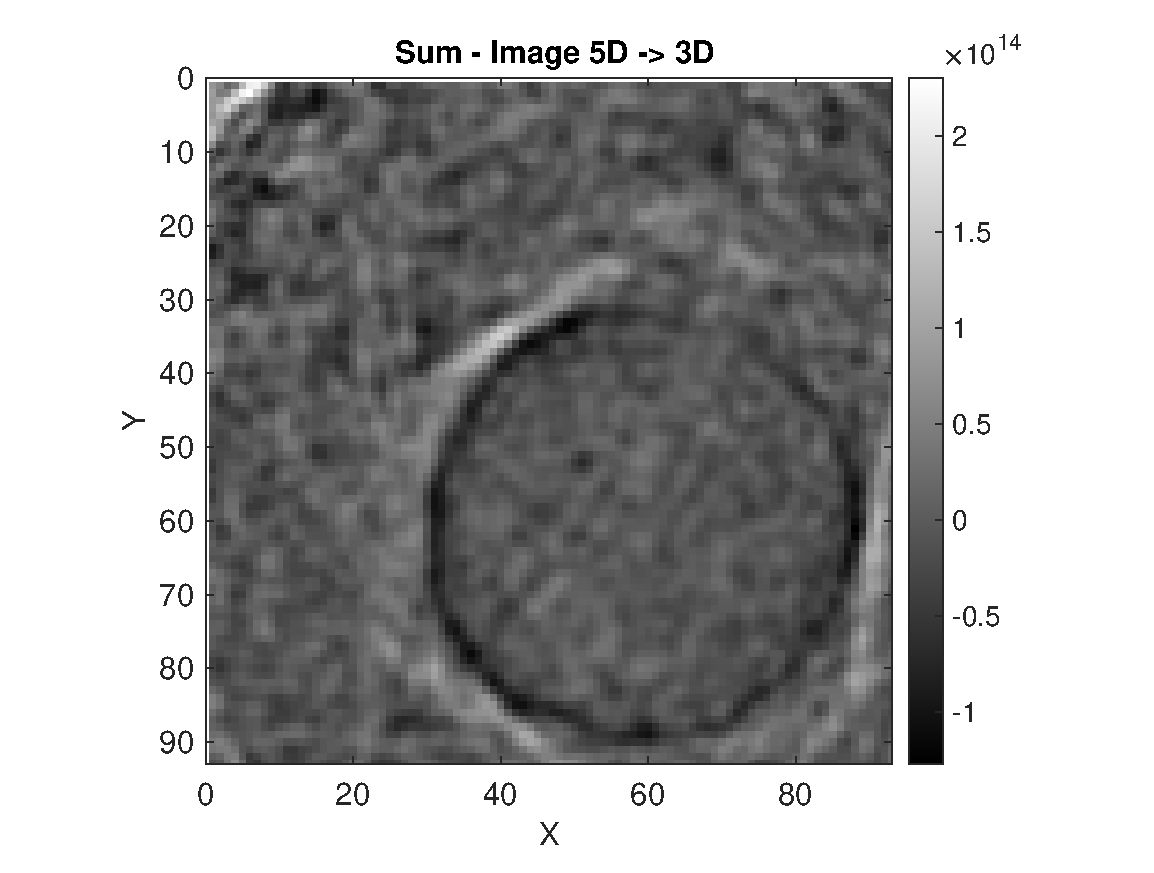
\includegraphics[width=1.09\linewidth]{Graphics/Results/Variance_Image/Variance_Ortho_slice_87_compare_5d_to_3d.eps}
         \caption{Slice thorough the 3D image which was constructed for the summation of the 4th and 5th dimension. }
         \label{fig:res:compare_normal_variance_normal}
     \end{subfigure}
     \hfill
     \begin{subfigure}[b]{0.47\textwidth}
         \centering
         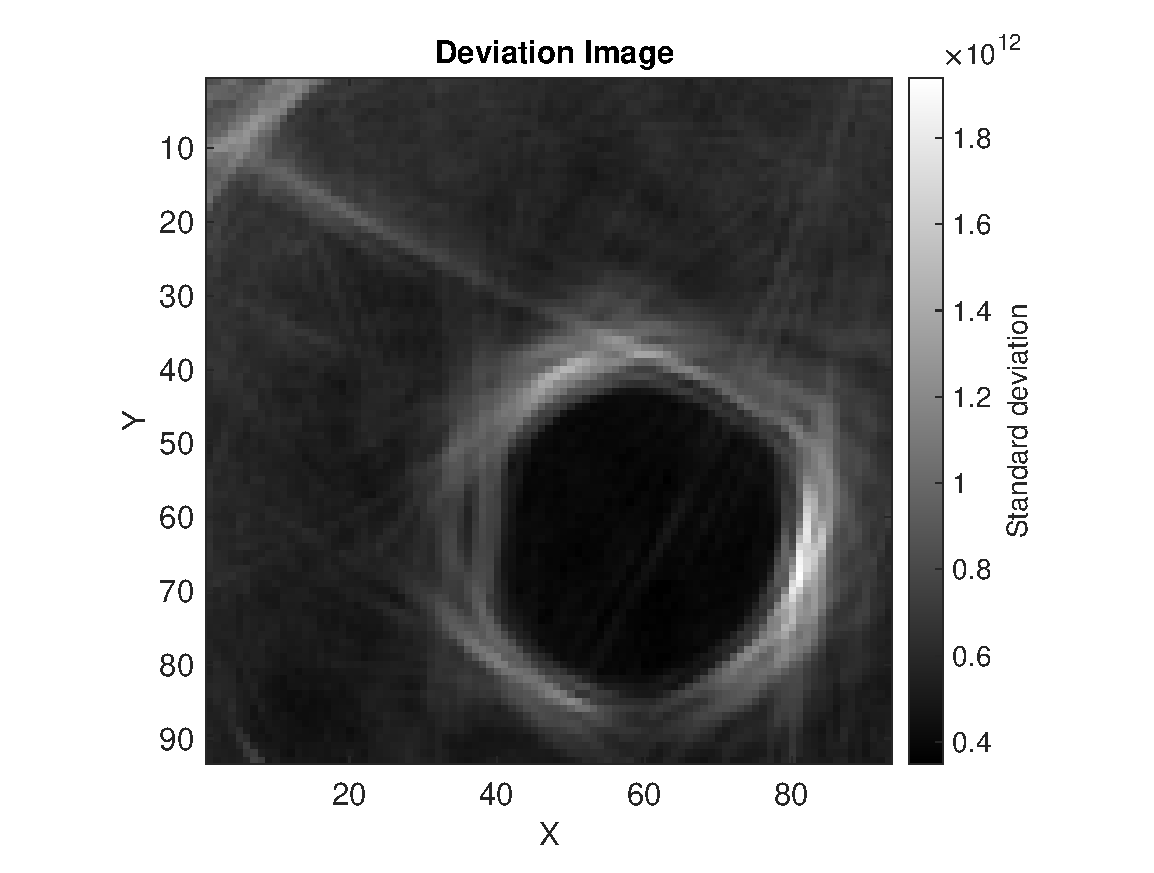
\includegraphics[width=1.13\textwidth]{Graphics/Results/Variance_Image/Variance_Ortho_slice_87.eps}
         \caption{Slice through the Deviation image. }
         \label{fig:res:compare_normal_variance_variance}
     \end{subfigure}
        \caption{Side by side comparison of the summarised 3D image to the Deviation image.}
        \label{fig:res:compare_normal_variance}
\end{figure}


Compared to the sum-image on the left the Figure \ref{fig:res:compare_normal_variance_variance} shows a much higher contrast. The stone in the middle as well as the part of the olive skin in the top left corner are clearly visible. The speckle artefacts are practically gone and the background value is close to zero. In section \ref{sec:res:eval_diff_tissue_type} the data for three different test voxels were shown. One was located at the top left corner of the reconstructed image and was placed on the skin of the olive. The second was placed directly in the pulp of the olive and the third was located at the stone in the centre of the olive. For the voxel located at the stone and the skin a specular behaviour was observed. For the voxel located in the pulp diffuse properties were noticed. The Deviation image shows that voxels located in tissue with high specularity show also a high standard deviation. Those parts are highlighted in the image and are easily distinguishable from the voxels with diffuse properties which appear very dark in the Deviation image. 


\begin{figure}[H]
        \centering
    \begin{subfigure}[b]{0.61\textwidth}
         \centering
         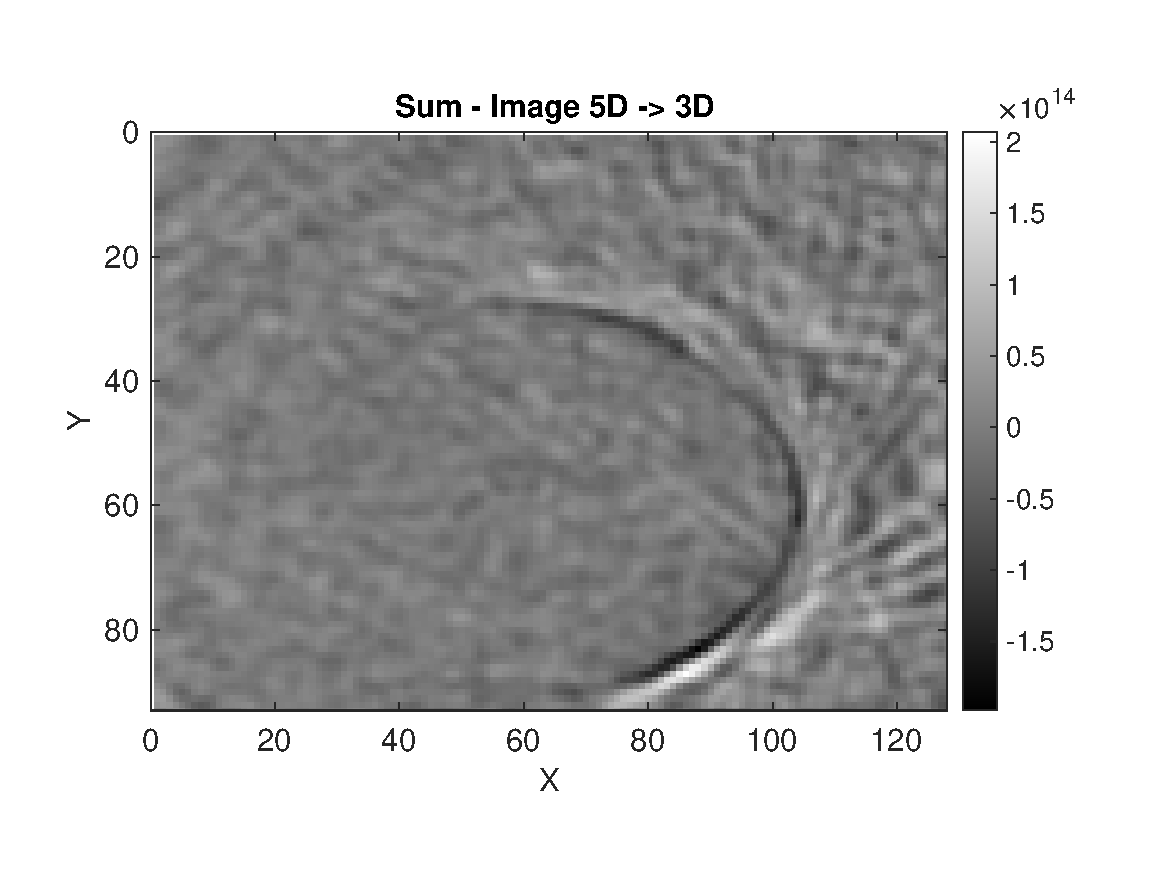
\includegraphics[width=1.13\textwidth]{Graphics/Results/Variance_Image/Variance_Ortho_slice_63_x_direkt_compare_5d_to_3d.eps}
         \caption{Summation image. }
         \label{fig:deviation_image_x_slice_normal}
     \end{subfigure}
     \hfill
    \begin{subfigure}[b]{0.61\textwidth}
        \centering
        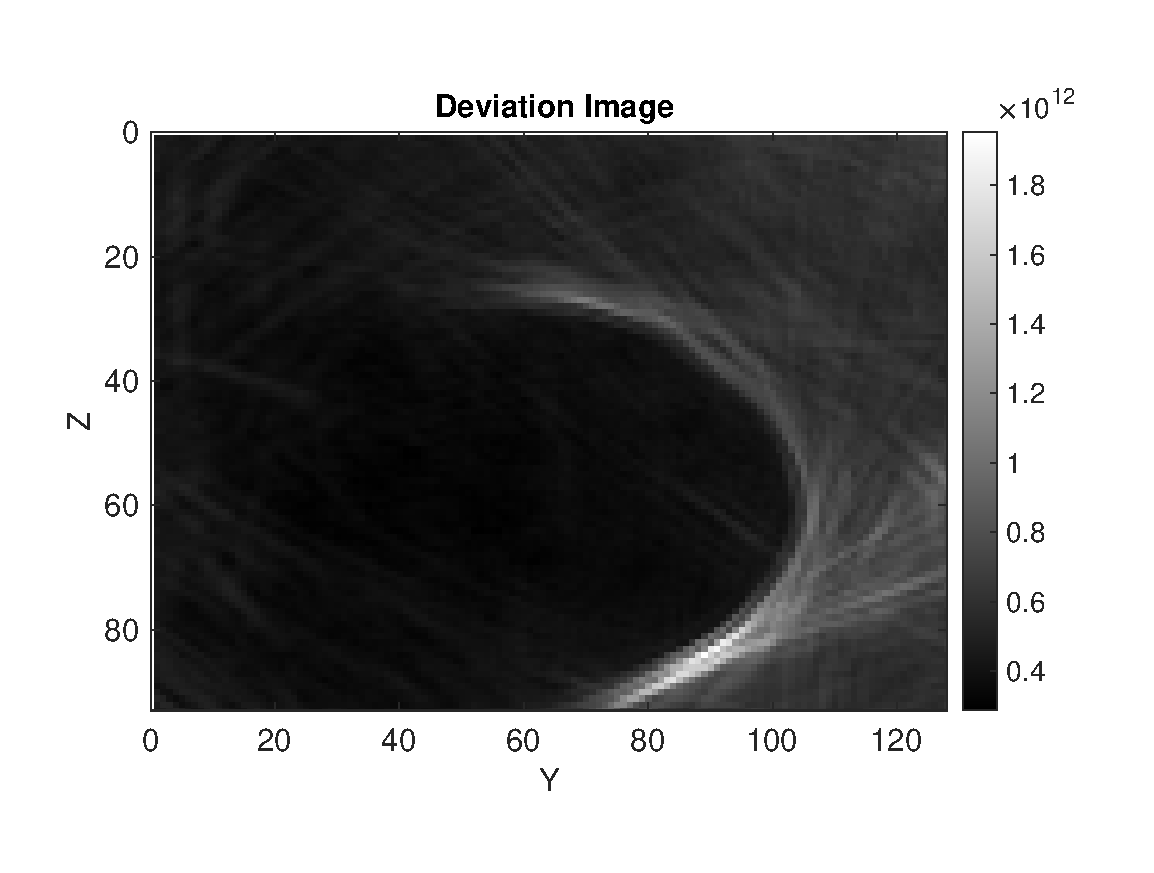
\includegraphics[width=1.13\textwidth]{Graphics/Results/Variance_Image/Variance_Ortho_slice_x_63.eps}
        \caption{Deviation image.}
        \label{fig:deviation_image_x_slice_deviation}
     \end{subfigure}
        \caption{Comparison of the Deviation image and the summation image. Sliced in x-direction. The oval in the middle of the image is part of the stone of the olive.}
        \label{fig:deviation_image_x_slice}
\end{figure}

In Figure \ref{fig:deviation_image_x_slice} the deviation image is shown from the side of the olive. This time the slices were made through the y-z-plain. Again, the edges of the stone of the olive are visible with higher contrast compared to the the summation image in Figure \ref{fig:deviation_image_x_slice_normal}. 


\bigskip
\bigskip



Using the \textbf{maximum values} of each of the 5D-4D-images leads to an alternative representation of the data. 

The highest peak of the 5D-4D-data is saved at the position of each voxel in the 3D image. The resulting images are shown in the following Figure:


\begin{figure}[H]
        \centering
    \begin{subfigure}[b]{0.61\textwidth}
         \centering
         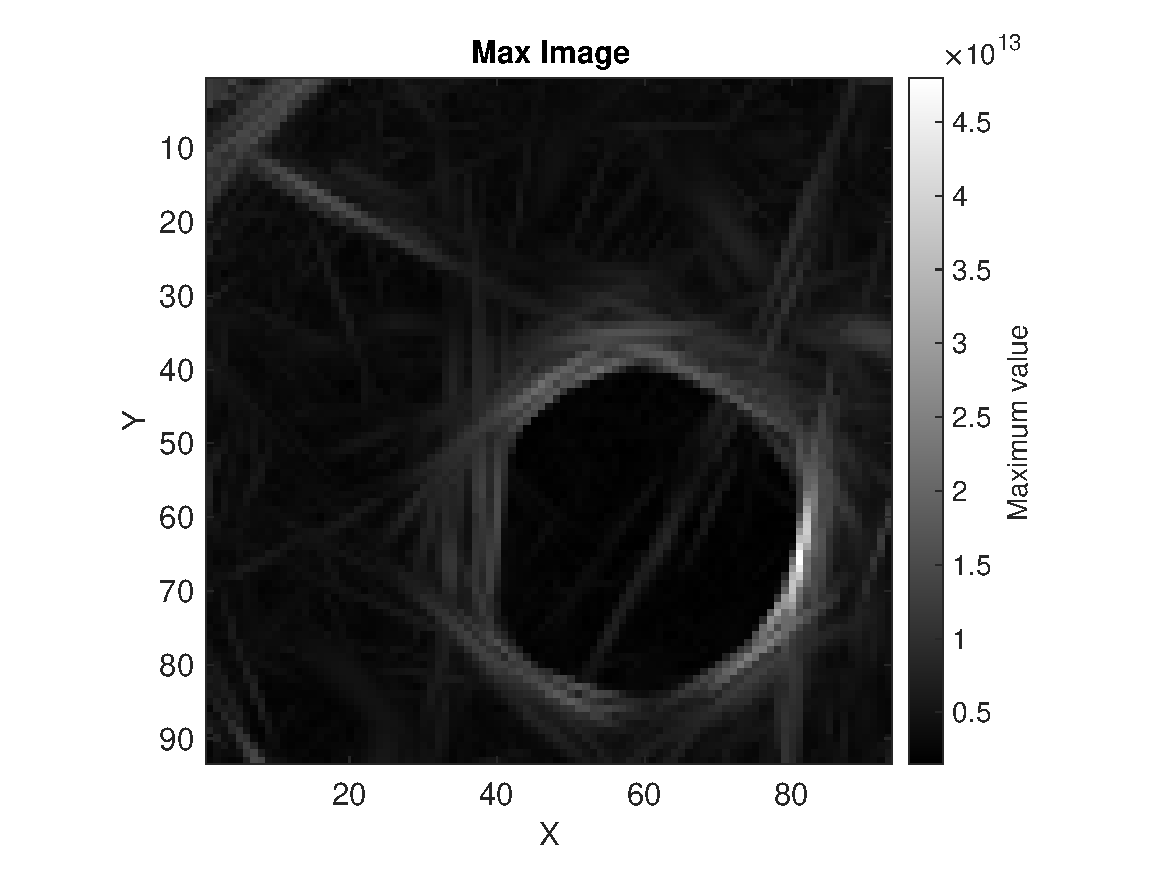
\includegraphics[width=1.13\textwidth]{Graphics/Results/Variance_Image/Max_Ortho_slice_87.eps}
         \caption{Max-Image seen from z-direction. }
         \label{fig:max_image_z-direct}
     \end{subfigure}
     \hfill
    \begin{subfigure}[b]{0.61\textwidth}
        \centering
        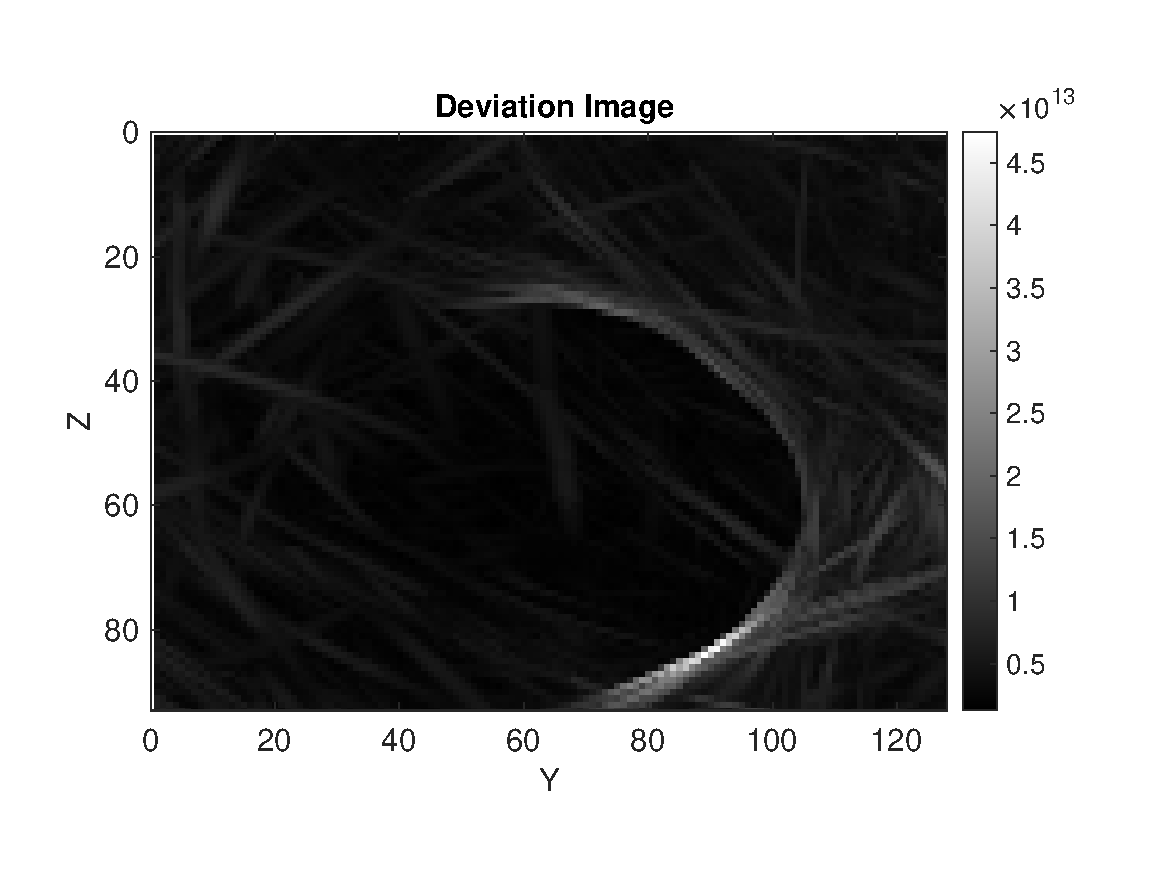
\includegraphics[width=1.13\textwidth]{Graphics/Results/Variance_Image/Max_Ortho_slice_x_63.eps}
        \caption{Max-Image seen from x-direction. }
        \label{fig:max_image_x_direkt}
     \end{subfigure}
        \caption{Max-Image as a representation of the five dimensional data in 3D.}
        \label{fig:max_image}
\end{figure}

Figure \ref{fig:max_image_z-direct} shows the maximum image with the same sectioning as the deviation image. The stone in the middle of the olive again is highlighted by the method. It was shown in Figure \ref{fig:res:5D_4D_skin_pulp_compare} that for the specular cases the 5D-4D-representation had multiple values on the leading diagonal which led to high peaks and an overall lower values for the other values besides the diagonal. In the specular case the ultrasonic pulses are reflected directly from the emitter direction into the receivers that lay in the same direction. Therefore, the pulses travel only a short distance and have little interaction with surrounding matter. For these cases the reflections cause a higher amplitude in the \ac{ascan} compared to a diffuse reflection where a big part of the energy is scattered into other directions. Therefore, the max-imaging technique also leads to a highlighted representation of mainly specular tissue. 




      
\section{Influence of the speed of sound correction }
In this section the influence of the \ac{sos} correction on the images shall be shown. For the following results 14 directional vectors were used during the reconstruction. For the first comparison the sum images of the 5D reconstruction can be seen.


\begin{figure}[H]
     \centering
     \begin{subfigure}[b]{0.47\textwidth}
                  \centering
         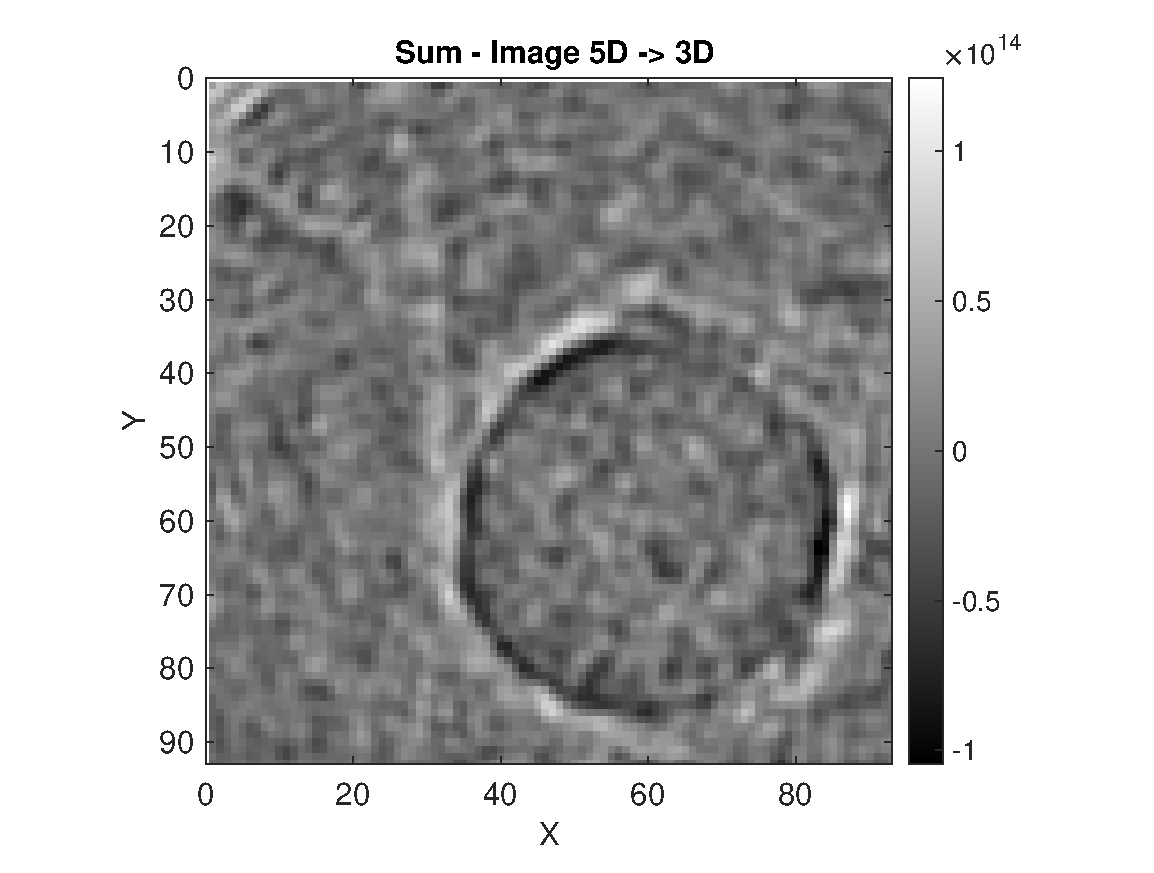
\includegraphics[width=1.09\textwidth]{Graphics/Results/14_vecs_sos_vs_noSos/sum_14vecs_no_sos_z_direction.eps}
         \caption{Without \ac{sos} correction.}
         \label{sos:influence_sum_images_without}
     \end{subfigure}
     \hfill
     \begin{subfigure}[b]{0.47\textwidth}
         \centering
         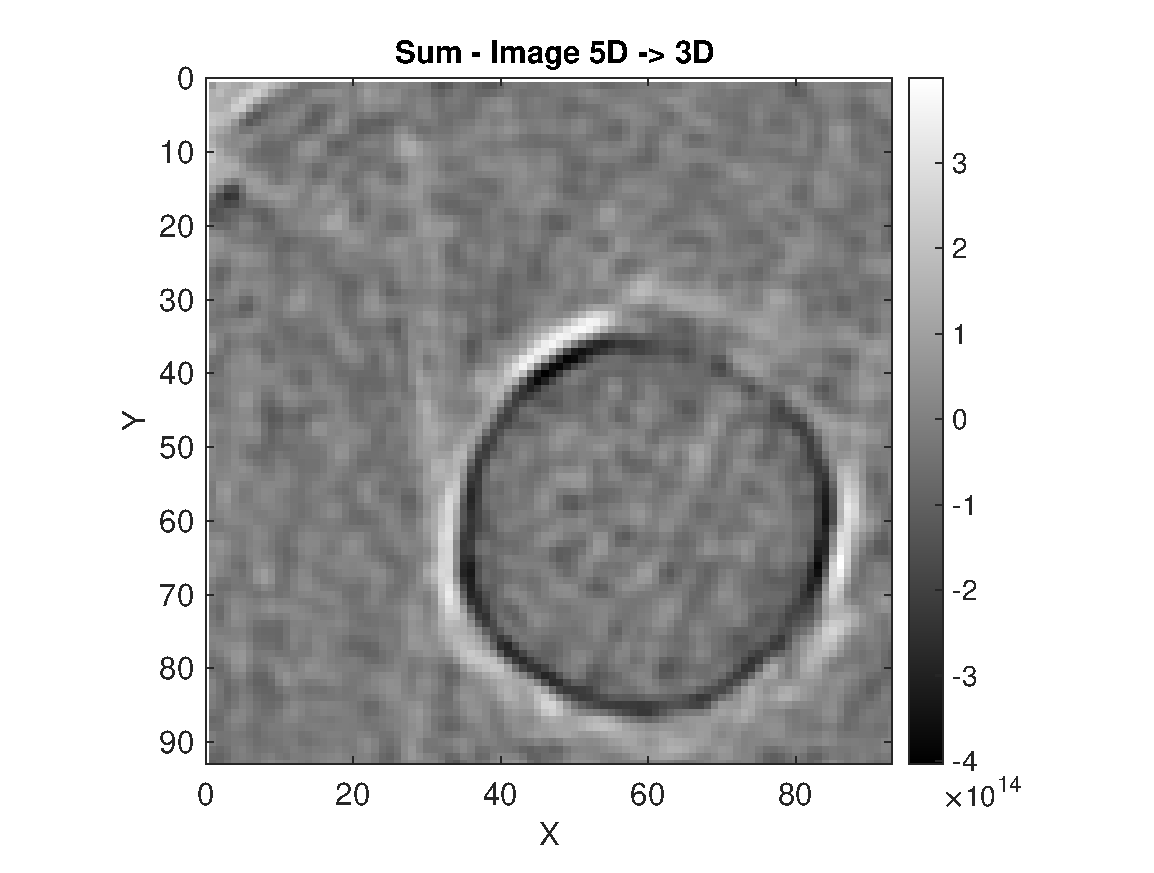
\includegraphics[width=1.09\linewidth]{Graphics/Results/14_vecs_sos_vs_noSos/sum_14vecs_with_sos_z_direction.eps}
         \caption{With \ac{sos} correction. }
         \label{sos:influence_sum_images_with}
     \end{subfigure}
        \caption{Influence of the \ac{sos} correction on the summarised image of 5D reconstruction.}
        \label{sos:influence_sum_images}
\end{figure}

It is visible on the first glance that the influence of the artefacts could be reduced. The reason for the lower visibility of the noise is the higher amplitude of the voxel values where actual image information is stored. The Figure \ref{influence_sum_images_with} shows a nearly two times higher amplitude compared to the image on the left. Therefore, the impact of the artefact could be reduced with the introduction of the \ac{sos} correction.

\bigskip

The 5D-over-4D images for the four different materials mentioned in section \ref{sec:input_data} are presented in the Figure \ref{fig:influence_sos_1} and \ref{fig:influence_sos_2}.
\begin{figure}[H]
     \centering
     \begin{subfigure}[b]{0.47\textwidth}
         \centering
         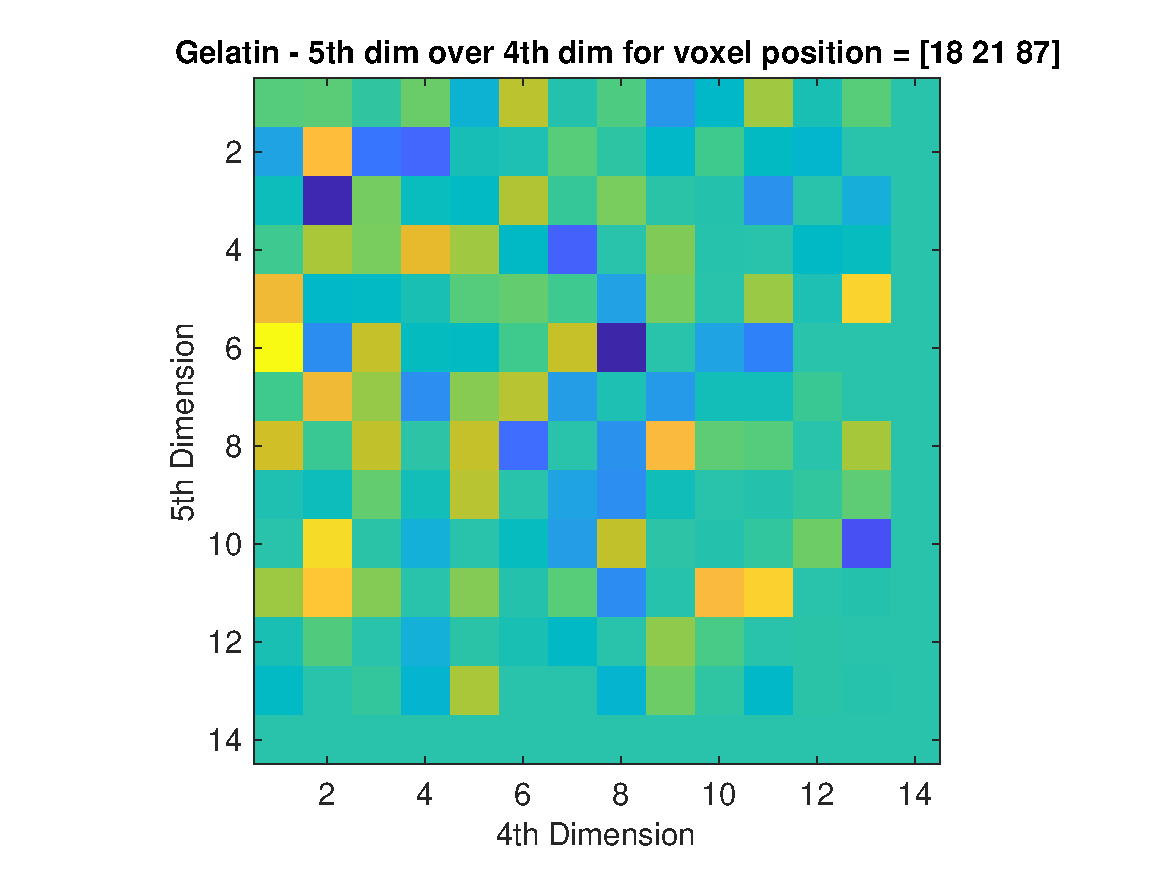
\includegraphics[width=1.02\linewidth,left]{Graphics/Results/14_vecs_sos_vs_noSos/5thdim_over4D_no_sos_pulp.eps}
         \caption{Without \ac{sos} correction. }
         \label{leer}
     \end{subfigure}
     \hfill
     \begin{subfigure}[b]{0.47\textwidth}
         \centering
         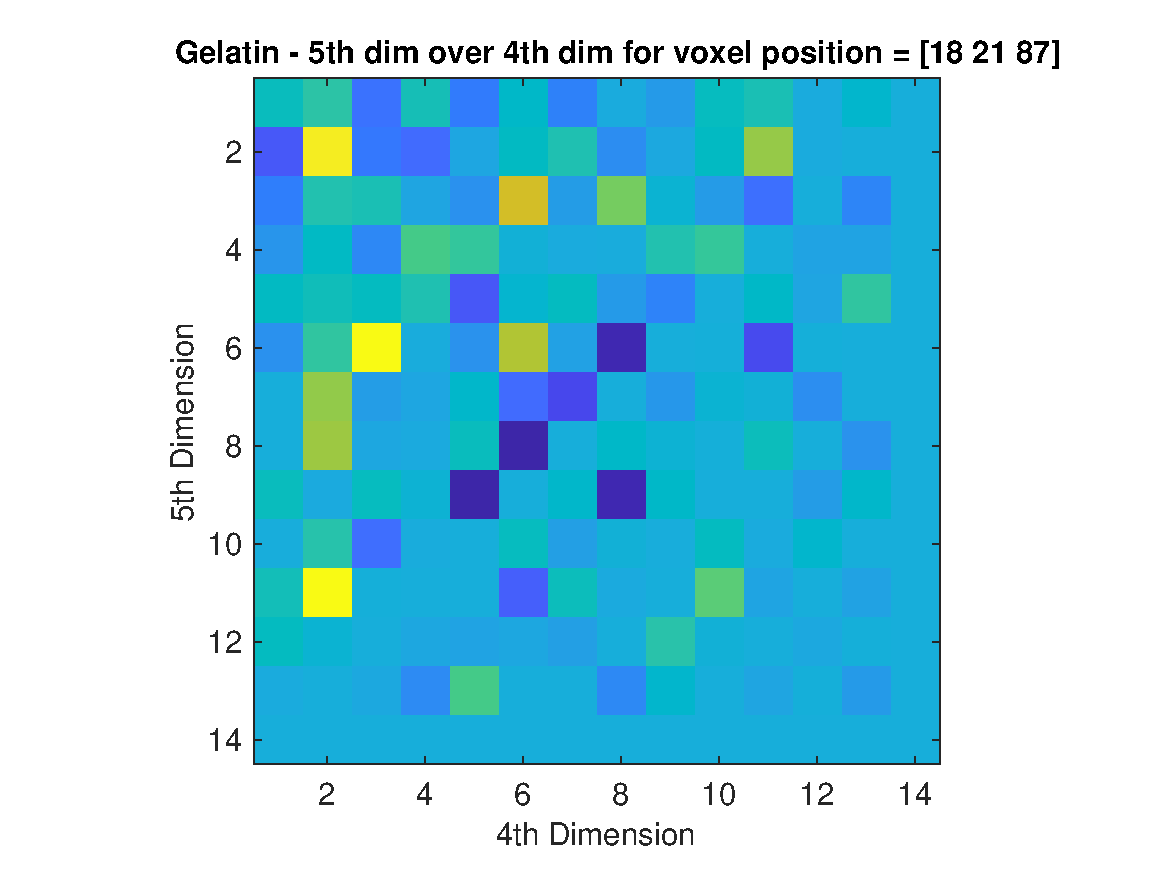
\includegraphics[width=1.02\textwidth]{Graphics/Results/14_vecs_sos_vs_noSos/5thdim_over4D_with_sos_pulp.eps}
         \caption{With \ac{sos} correction.}
         \label{leer}
     \end{subfigure}
          \hfill
     \begin{subfigure}[b]{0.47\textwidth}
         \centering
         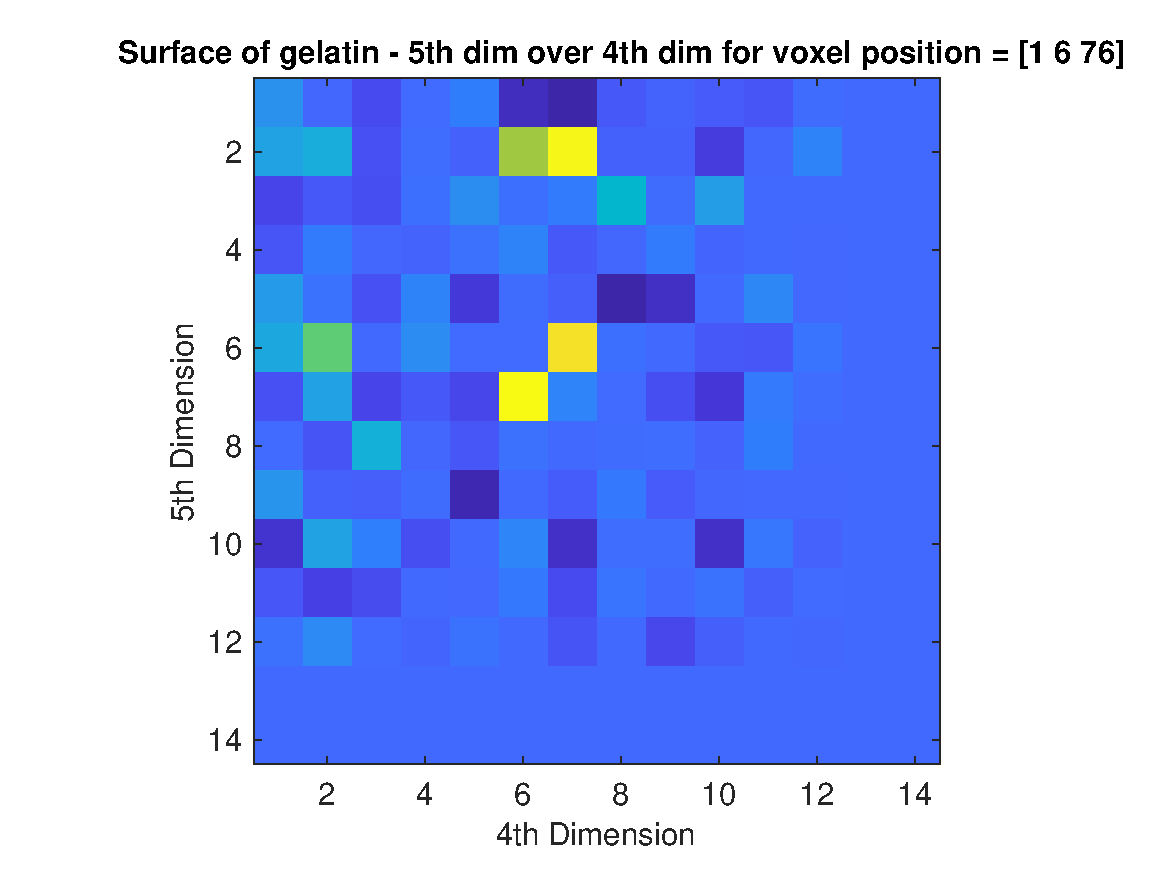
\includegraphics[width=1.02\textwidth]{Graphics/Results/14_vecs_sos_vs_noSos/5thdim_over4D_no_sos_skin.eps}
         \caption{Without \ac{sos} correction.}
         \label{leer}
     \end{subfigure}
          \hfill
     \begin{subfigure}[b]{0.47\textwidth}
         \centering
         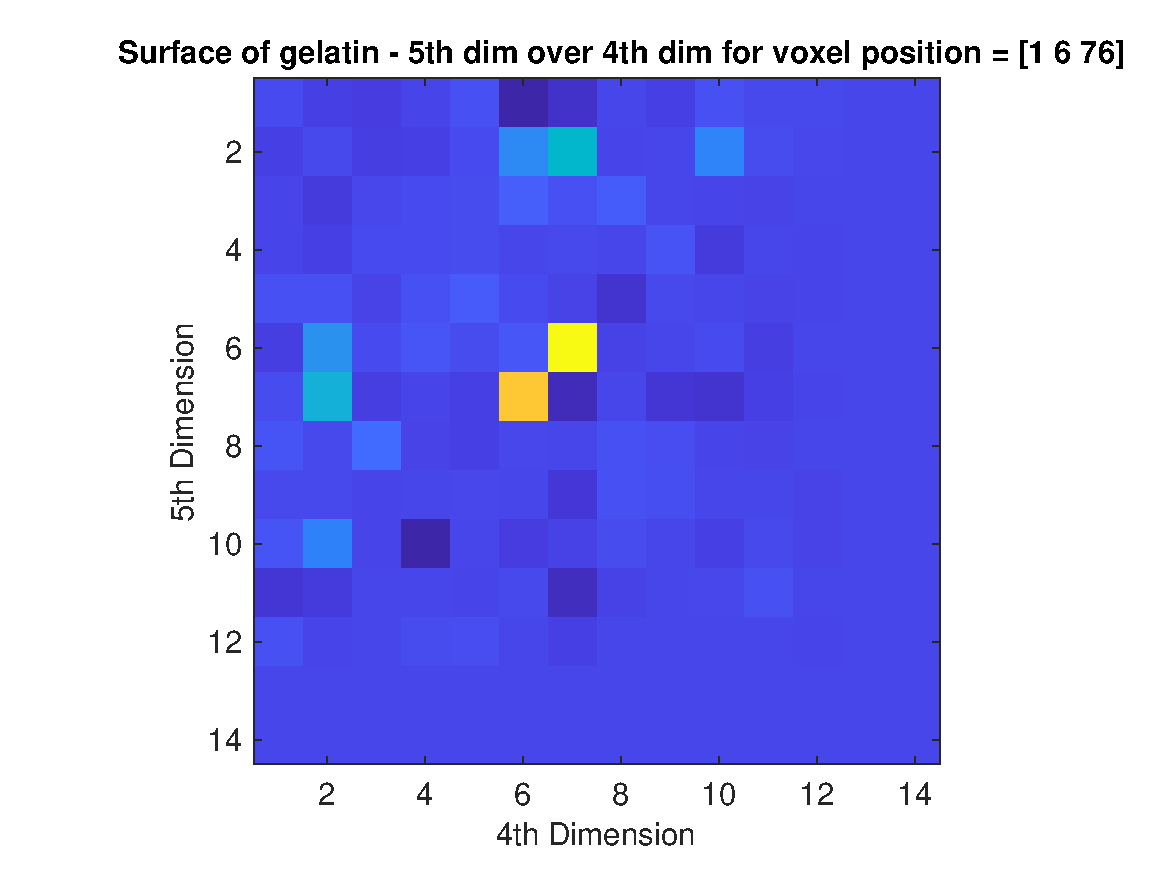
\includegraphics[width=1.02\textwidth]{Graphics/Results/14_vecs_sos_vs_noSos/5thdim_over4D_with_sos_skin.eps}
         \caption{With \ac{sos} correction.}
         \label{leer}
     \end{subfigure}
        \caption{Influence of the \ac{sos} correction on the 5D-over-4D-representation of reconstructed image with 14 directional vectors. The images on the left are reconstructed without the \ac{sos} correction. The results on the right are generated while considering the speed of sound.}
        \label{fig:influence_sos_1}
\end{figure}

These results are only compared qualitatively. It was mentioned in the section \ref{sec:res:eval_diff_tissue_type} that it is assumed that tissue types or materials with specular reflection characteristics have a symmetrical 5D-over-4D representation for that particular voxel. The symmetry can be enhanced by applying the \ac{sos} correction. The peak values are increased so that the artefacts have a smaller influence. This makes them more prominent in the 4D-over-5D representation and brings out the symmetry even more. 

\begin{figure}[H]
     \centering
      \hfill
     \begin{subfigure}[b]{0.45\textwidth}
         \centering
         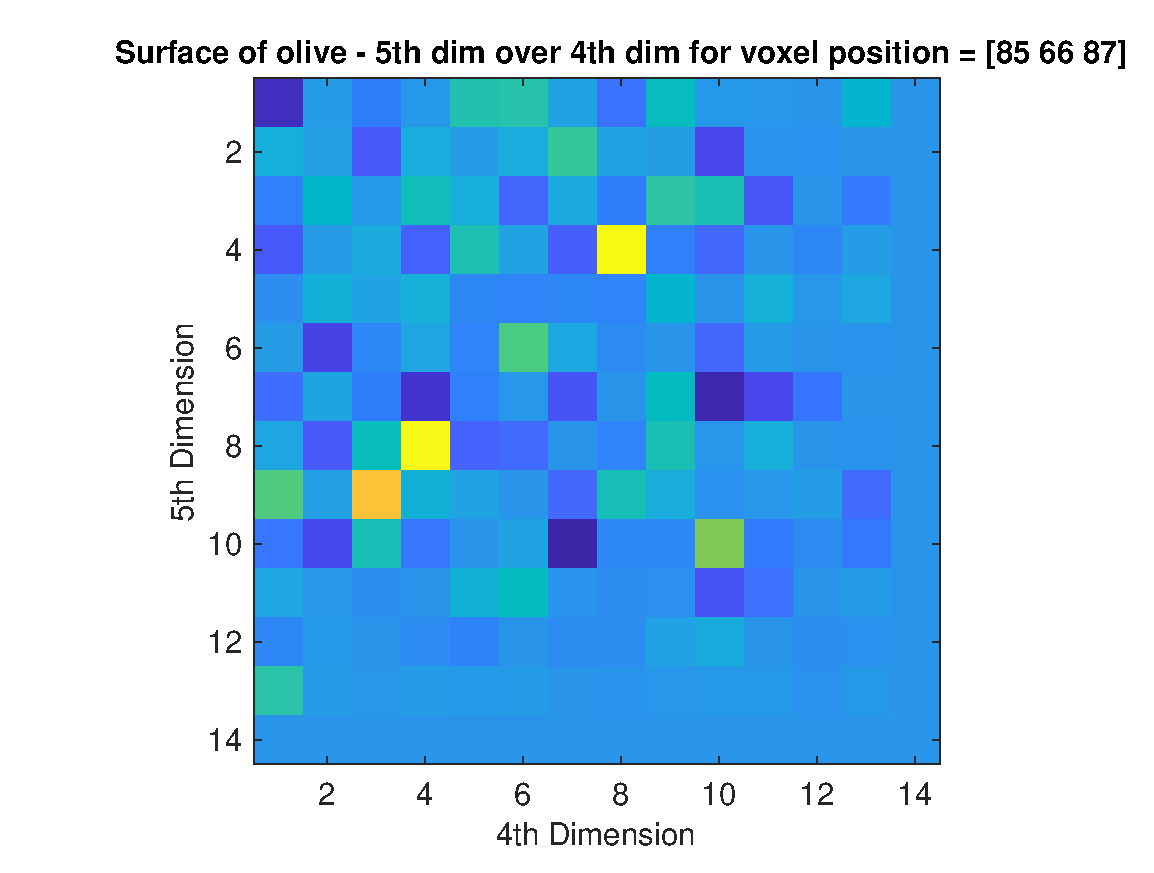
\includegraphics[width=1.02\textwidth,right]{Graphics/Results/14_vecs_sos_vs_noSos/5thdim_over4D_no_sos_stone.eps}
         \caption{Without \ac{sos} correction.}
         \label{fig:influence_sos_2_a}
     \end{subfigure}
          \hfill
     \begin{subfigure}[b]{0.47\textwidth}
         \centering
         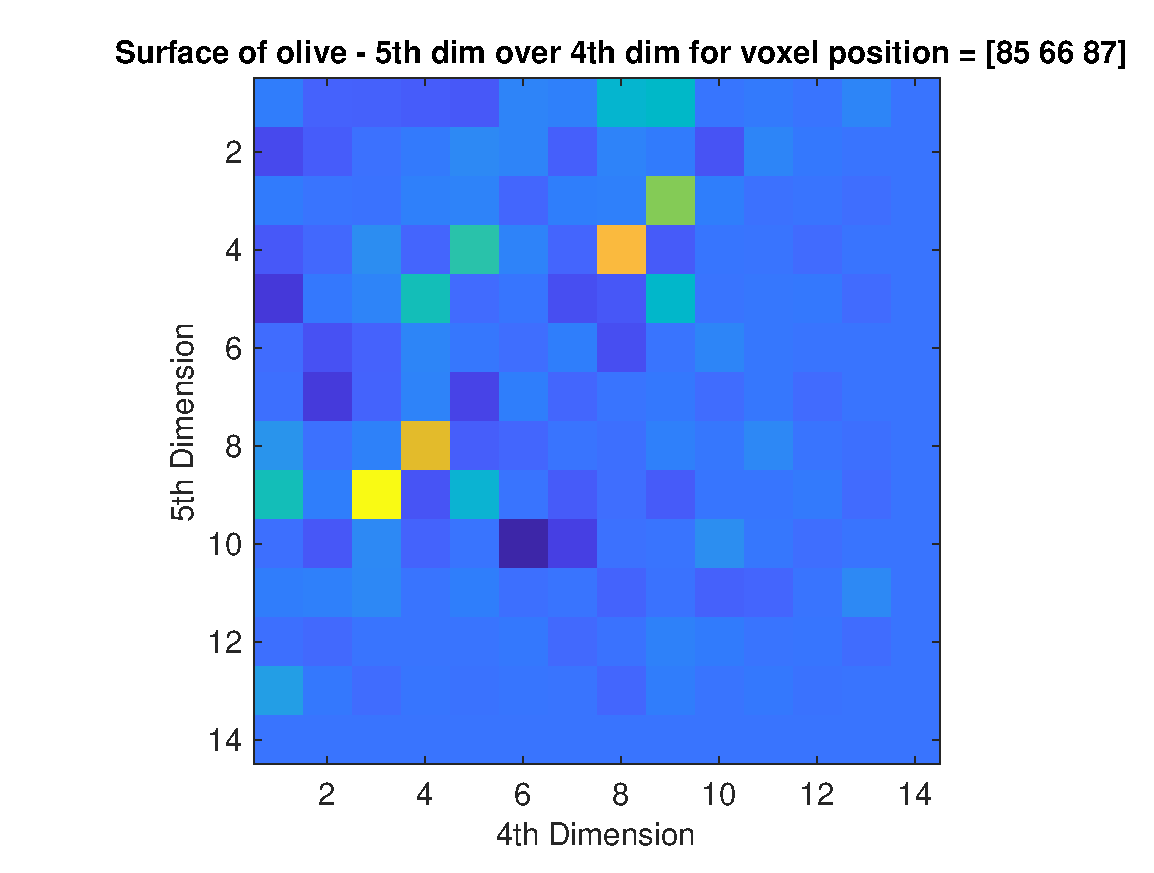
\includegraphics[width=1.02\textwidth]{Graphics/Results/14_vecs_sos_vs_noSos/5thdim_over4D_with_sos_stone.eps}
         \caption{With \ac{sos} correction.}
         \label{fig:influence_sos_2_b}
     \end{subfigure}
          \hfill
     \begin{subfigure}[b]{0.47\textwidth}
         \centering
         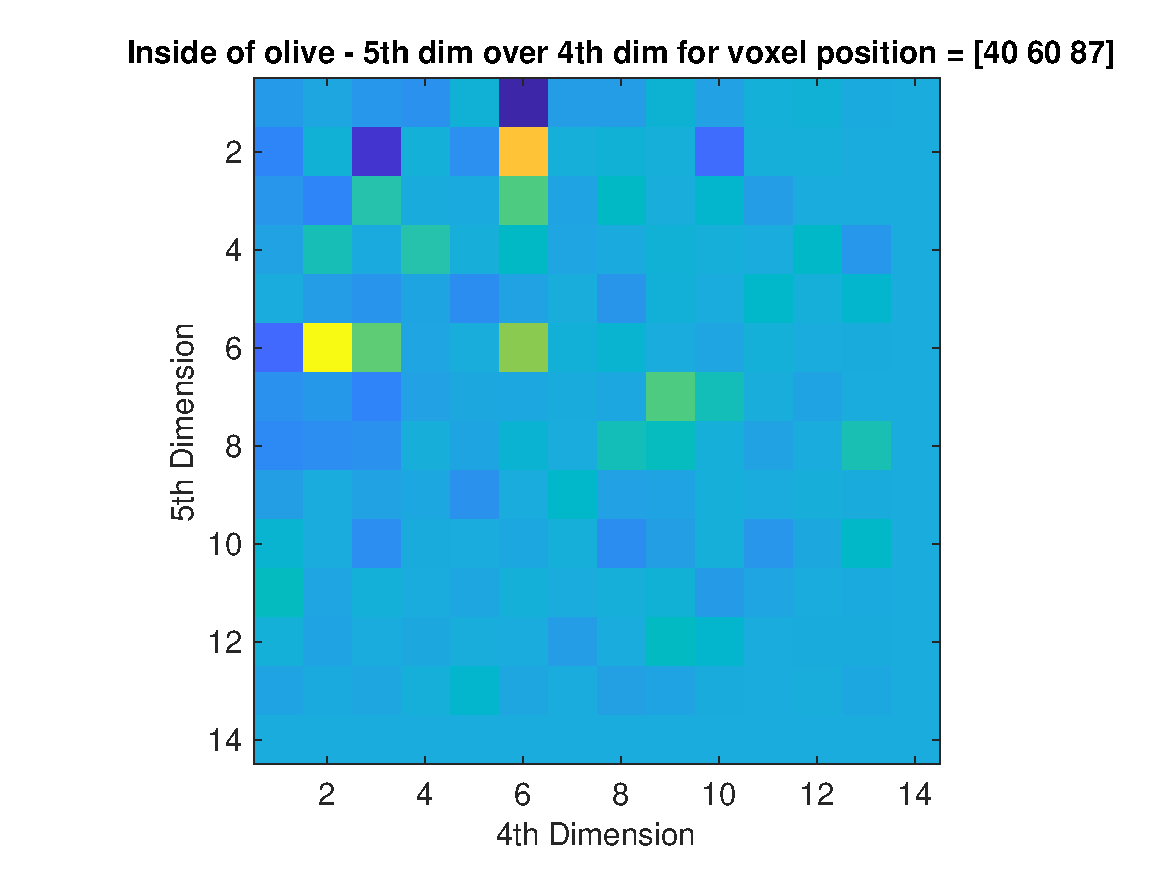
\includegraphics[width=1.02\textwidth]{Graphics/Results/14_vecs_sos_vs_noSos/5thdim_over4D_no_sos_inside_olive.eps}
         \caption{Without \ac{sos} correction.}
         \label{leer}
     \end{subfigure}
          \hfill
     \begin{subfigure}[b]{0.47\textwidth}
         \centering
         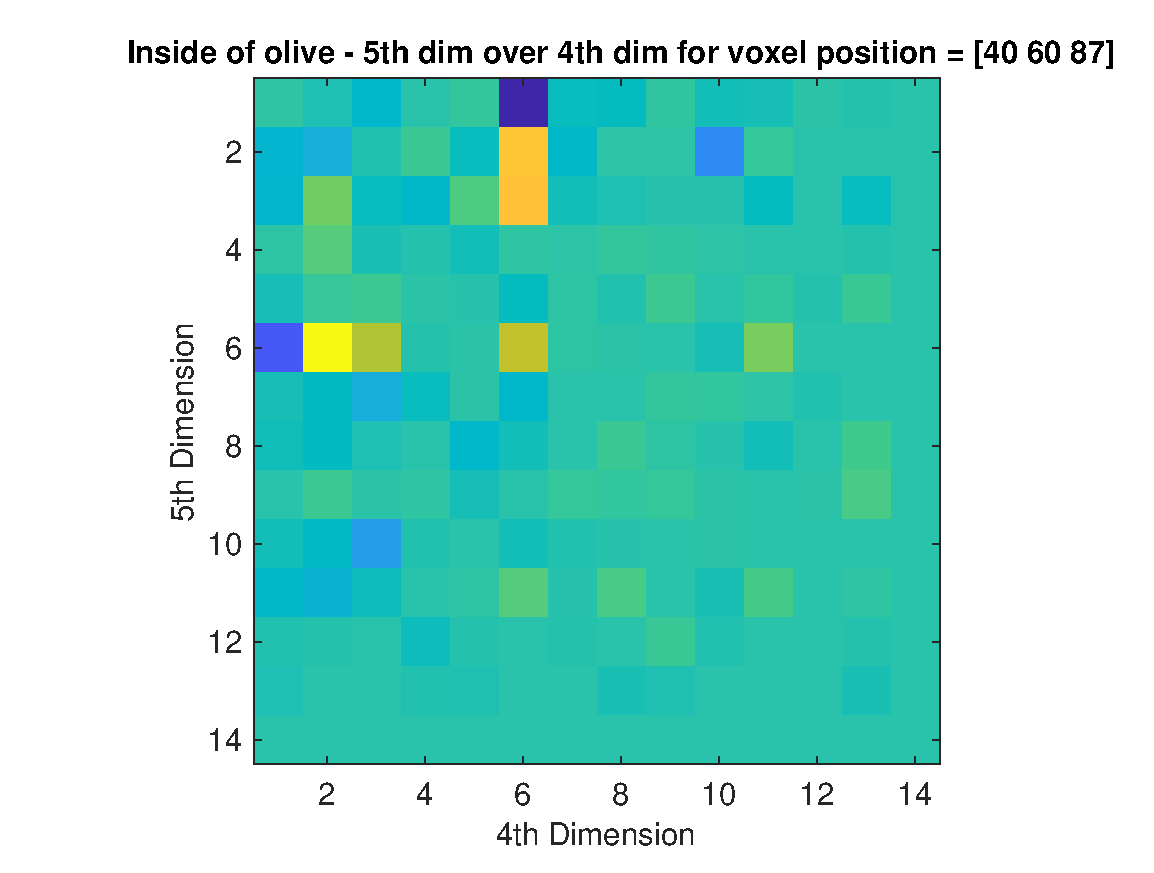
\includegraphics[width=1.02\textwidth]{Graphics/Results/14_vecs_sos_vs_noSos/5thdim_over4D_with_sos_inside_olive.eps}
         \caption{With \ac{sos} correction.}
         \label{leer}
     \end{subfigure}
        \caption{Influence of the \ac{sos} correction on the 5D-over-4D-representation of reconstructed image with 14 directional vectors. The images on the left are reconstructed without the \ac{sos} correction. The results on the right are generated while considering the speed of sound.}
        \label{fig:influence_sos_2}
\end{figure}


The biggest effect on the symmetry enhancement can be observed in Figures \ref{fig:influence_sos_2_a} and \ref{fig:influence_sos_2_b} for the skin of the olive. The result on the left shows first signs of a symmetrical distribution of the voxel values but has a lot of other superimposing components. The underlying noise could successfully be compensated by the application of the \ac{sos} correction and the symmetry could be brought about. 


\begin{figure}[H]
     \centering
     \begin{subfigure}[b]{0.47\textwidth}
              \centering
         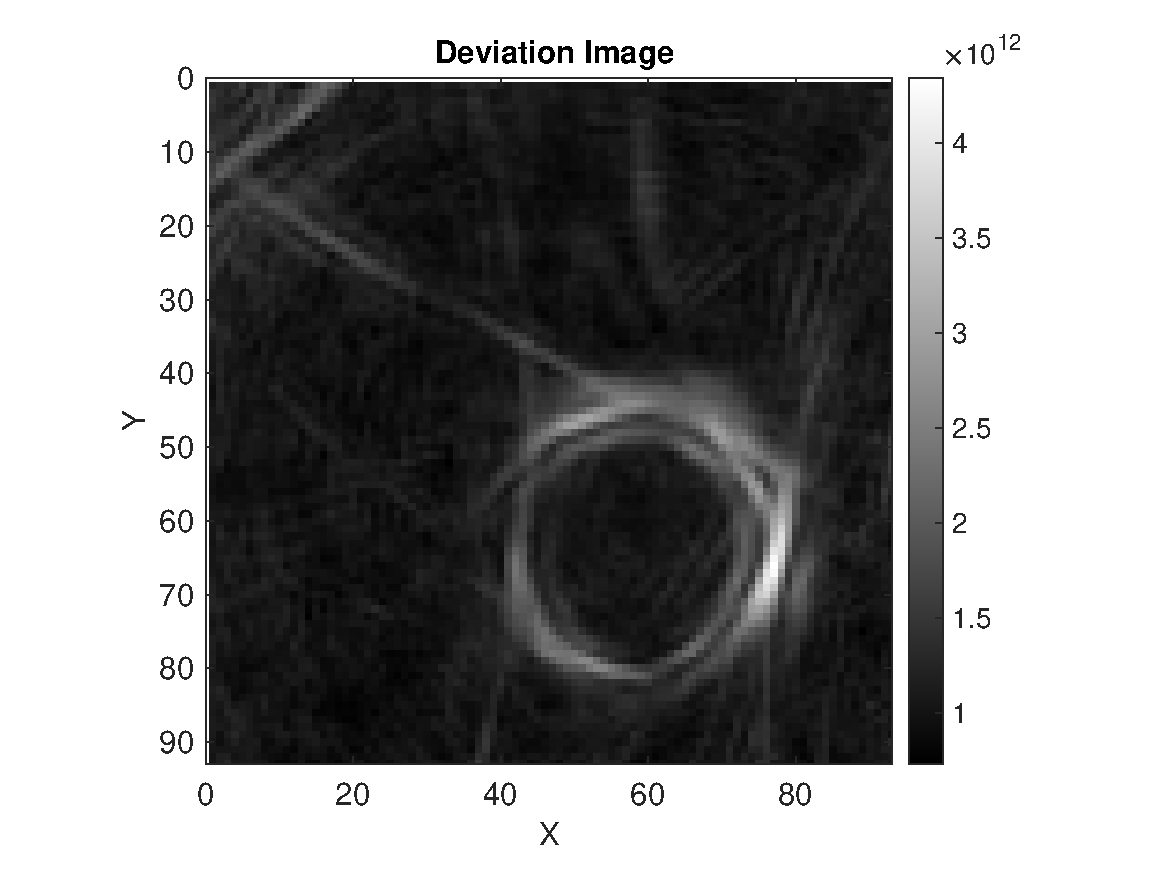
\includegraphics[width=1.09\textwidth]{Graphics/Results/14_vecs_sos_vs_noSos/Deviation_14vecs_no_sos_z_direction.eps}
         \caption{Without \ac{sos} correction.}
         \label{leer}
     \end{subfigure}
     \hfill
     \begin{subfigure}[b]{0.47\textwidth}
         \centering
         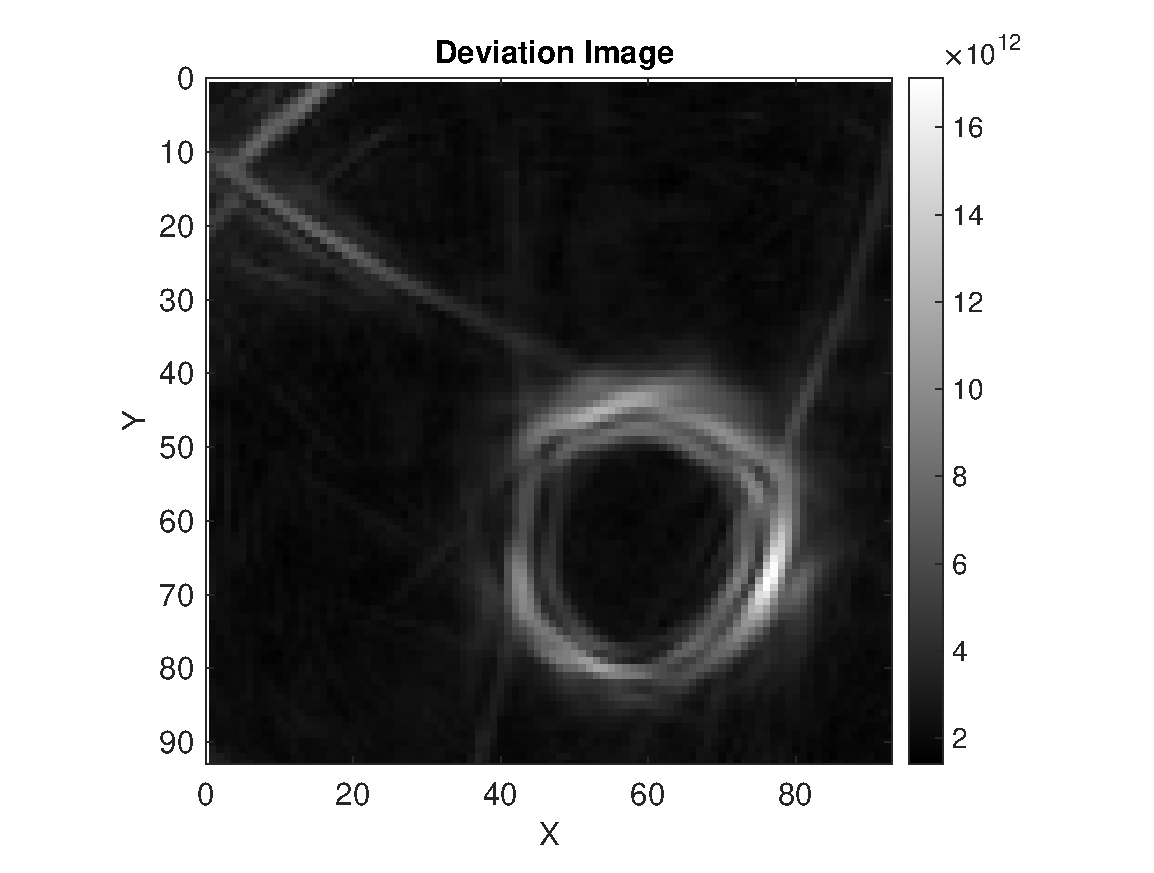
\includegraphics[width=1.09\linewidth]{Graphics/Results/14_vecs_sos_vs_noSos/Deviation_14vecs_with_sos_z_direction.eps}
         \caption{With \ac{sos} correction. }
         \label{leer}
     \end{subfigure}
        \caption{Influence of the \ac{sos} correction on the deviation image.}
        \label{fig:influence_sos_on_deviation}
\end{figure}


The results for the deviation imaging were presented in section \ref{chap:devi_image}. This imaging method benefits also from the \ac{sos} correction. The comparison of the results with and without \ac{sos} correction are shown in Figure \ref{fig:influence_sos_on_deviation}. The contrast could be enhanced and the influence of noise reduced. 

\begin{figure}[H]
     \centering
     \begin{subfigure}[b]{0.47\textwidth}
                  \centering
         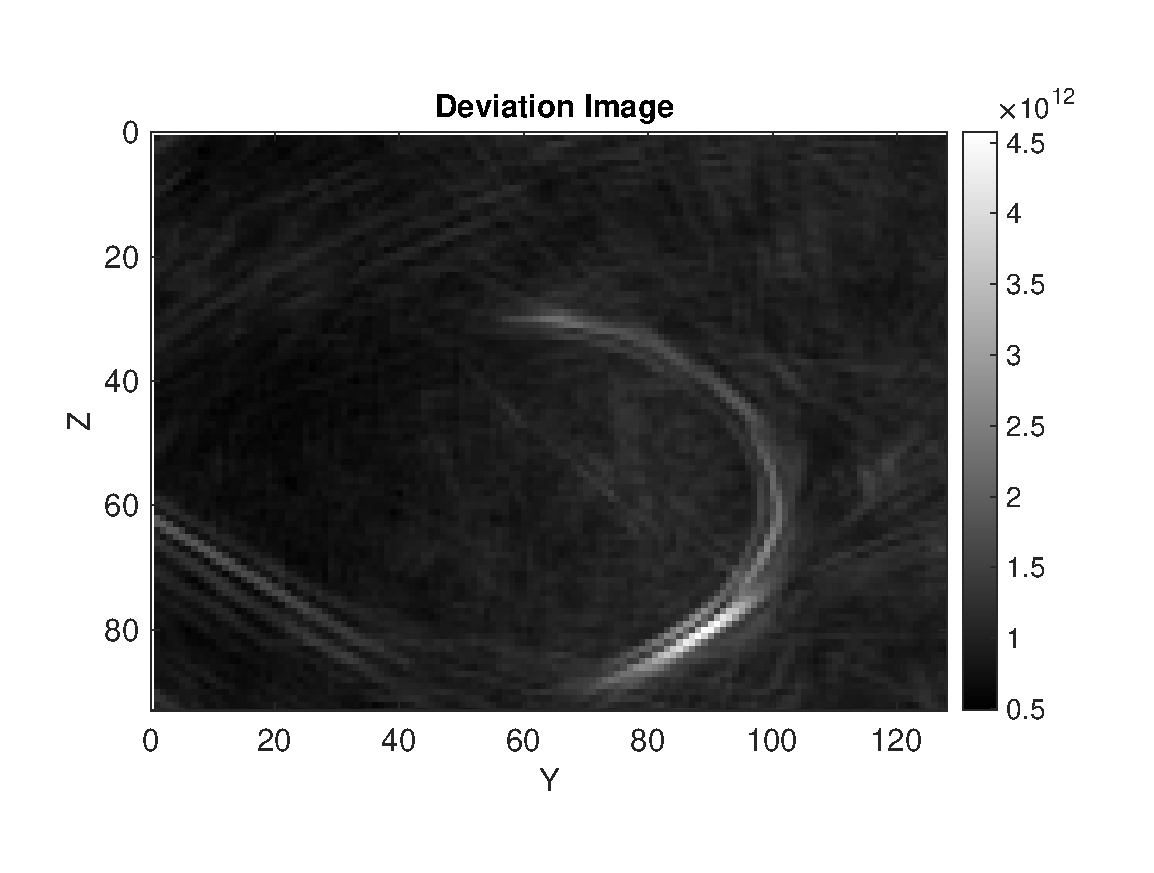
\includegraphics[width=1.09\textwidth]{Graphics/Results/14_vecs_sos_vs_noSos/Deviation_14vecs_no_sos_x_direction.eps}
         \caption{Without \ac{sos} correction.}
         \label{leer}
     \end{subfigure}
     \hfill
     \begin{subfigure}[b]{0.47\textwidth}
         \centering
         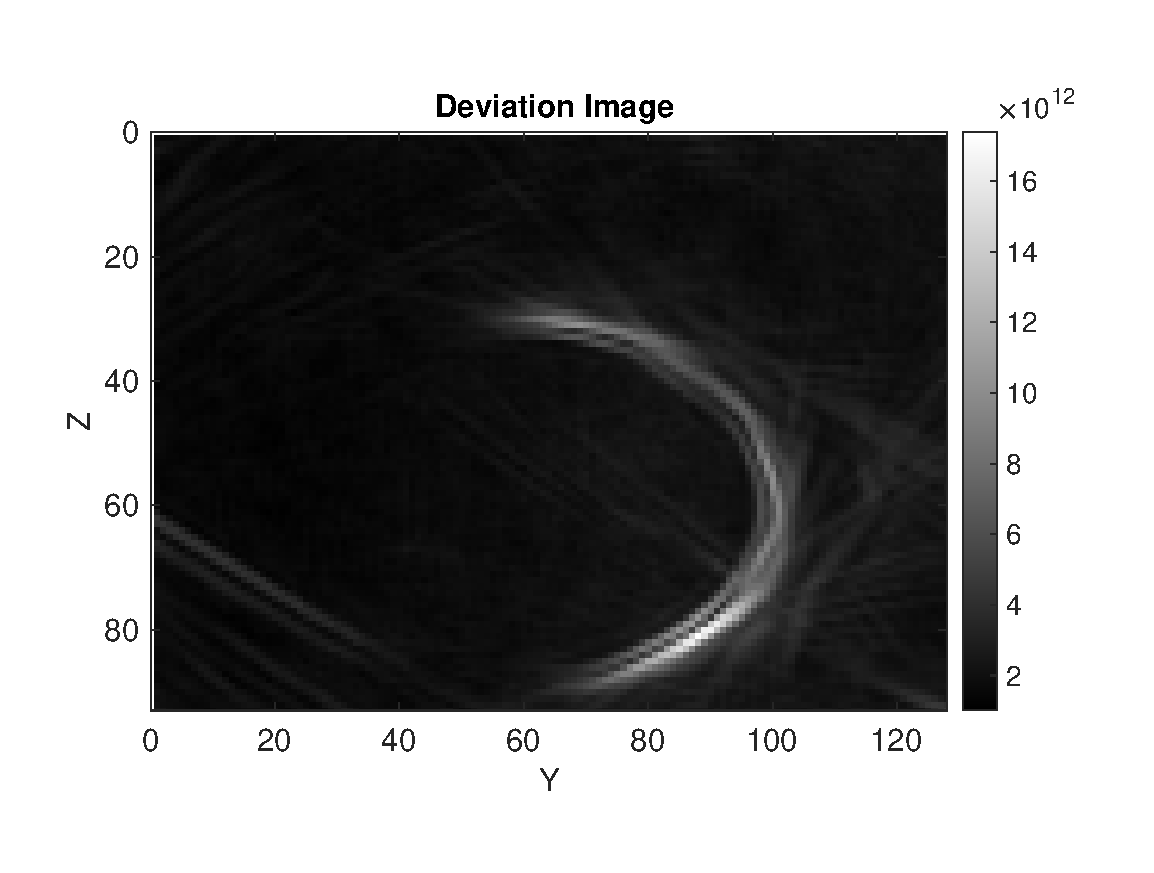
\includegraphics[width=1.09\linewidth]{Graphics/Results/14_vecs_sos_vs_noSos/Deviation_14vecs_with_sos_x_direction.eps}
         \caption{With \ac{sos} correction. }
         \label{leer}
     \end{subfigure}
        \caption{Influence of the \ac{sos} correction on the Deviation image.}
        \label{leer}
\end{figure}




\section{Angular relation between directional information}
\label{angular_directional_relation}


Until now the directional vectors could not be compared to each other properly. Their index was based on the order of their generation the angular relation between them was missing. A solution for this problem is presented in this section. A so called graticule is introduced. It is a representation of the azimuth and elevation of a spherical coordinate system in a 2 dimensional coordinate system. A simple example is shown in the following Figure:

\begin{figure}[H]
    \centering
    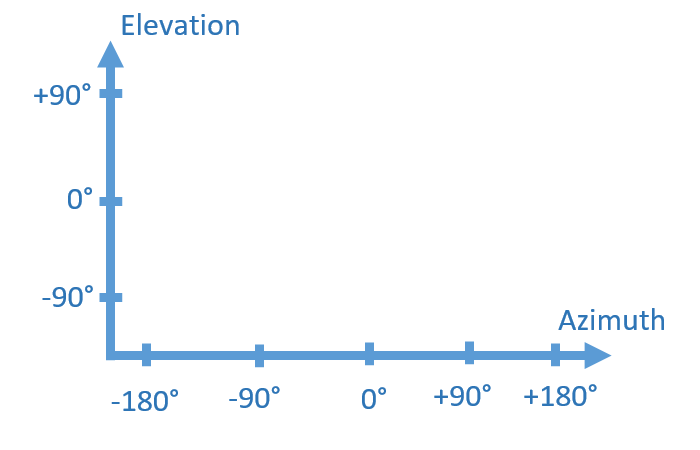
\includegraphics[width=0.76\textwidth]{Graphics/example_gradnetz.png}
    \caption{Basic representation of the graticule. The x-axis holds the information of the azimuth coordinate and the y-axis the information of the elevation. }
    \label{fig:gadnetz_example}
\end{figure}

With this representation the directional information of the single directional vectors now can be brought into a representative form so that the angular relationship between the data becomes visible. The 35 directional vectors that are used for the 5D reconstruction are shown in the following image: 

\begin{figure}[H]
    \centering
    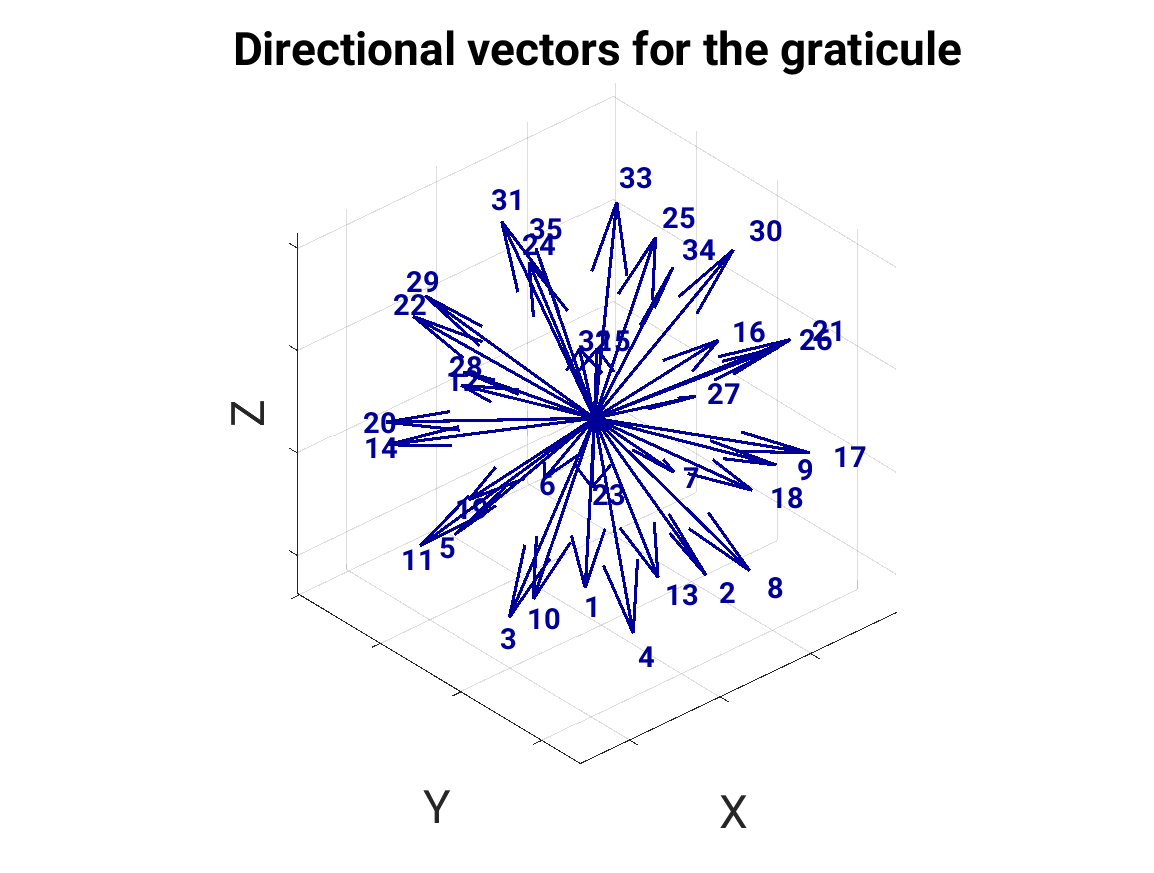
\includegraphics[width=0.76\textwidth]{Graphics/Results/gradnetz/directional_vectors_for_gradnetz.eps}
    \caption{The 35 directional vectors that shall be projected into the graticule. }
    \label{fig:gadnetz_directional_vectors}
\end{figure}

To transfer these directional vectors in the graticule the azimuth as well as the elevation is calculated for every direction vector. The resulting spherical coordinates are then plotted into the graticule. The values for the azimuth are plotted on the x-axis and the values for the elevation are assigned to the y-axis of the graticule. The result can be seen in the following image:

\begin{figure}[H]
    \centering
    \includegraphics[width=0.76\textwidth]{Graphics/Results/gradnetz/graticule_35_vectors.eps}
    \caption{The 35 directional vectors now presented in the graticule. The units are given in degrees. }
    \label{fig:fertig_gradnetz}
\end{figure}

From the representation in Figure \ref{fig:fertig_gradnetz} now the directional vectors can be regarded with their angular relation to each other. This shall be shown in the following example. A test voxel is defined with the voxel coordinates $[70\, , \, 82\, , \, 91]$. The coordinates for the test voxel are plotted in Figure \ref{fig:gadnetz_location_testvoxel}.

\begin{figure}[H]
    \centering
    \includegraphics[width=0.76\textwidth]{Graphics/Results/gradnetz/positionof_test_voxel_for-gradnetz.png}
    \caption{Location of the test voxel $[70\, , \, 82\, , \, 91]$ for the graticule. }
    \label{fig:gadnetz_location_testvoxel}
\end{figure}

The test voxel was chosen on the surface of the olive. This surface is assumed to have specular properties as first results in section \ref{sec:res:eval_diff_tissue_type} indicated. 

\bigskip

For the generation of the following results the data set from section \ref{sec:input_data} were used. The reconstruction of the 5D image was performed with the orthogonality threshold method and with 35 directional vectors. The graticule with image data can be seen in Figure \ref{fig:gadnetz_with_values}.



\begin{figure}[H]
     \centering
     \begin{subfigure}[b]{0.77\textwidth}
                  \centering
         \includegraphics[width=1.09\textwidth]{Graphics/Results/gradnetz/graticule_with_values.eps}
         \caption{Graticule with the values of the receiver data for all directional vectors which have their origin at the emitter direction 12.}
         \label{fig:gadnetz_with_value_values}
     \end{subfigure}
     \hfill
     \begin{subfigure}[b]{0.77\textwidth}
         \centering
         \includegraphics[width=1.09\linewidth]{Graphics/Results/gradnetz/graticule_35_vectors_emitter_12_active.eps}
         \caption{Graticule of the positions of the directional vectors. Vector 12 is marked red because the data of the graticule are used from the emitter direction 12.  }
         \label{fig:gadnetz_with_value_vecotrs}
     \end{subfigure}
        \caption{Influence of the \ac{sos} correction on the Deviation image.}
        \label{fig:gadnetz_with_values}
\end{figure}


For these results, the emitter direction was exemplarily chosen as 12. This means, that only the data is considered that was emitted from an emitter \ac{tas} that lay inside of the decision cone of directional vector 12. Furthermore, the receiver values for every direction are regarded. This means, that from all the data in the 5D image only the voxel values are regarded that originate from an emitter in direction 12. These voxel values then are placed into the graticule at the position of their corresponding receiver vectors and two dimensionally interpolated to create the image that we can see in Figure \ref{fig:gadnetz_with_value_values}. The colours of the figure represent the voxel value at that particular direction vector. The absolute value of the voxel values was chosen so that both positive and negative values of the \acp{ascan} are regarded. A bright structure is visible located at the position of the directional voxel 12. The structure results from the interpolation of the different voxel values located at the directional vectors surrounding vector 12. From the concentrated distribution of voxel values around the directional vector 12 the result can be interpreted as the result of a reflection on the surface of the olive with high specular properties. It remains to be examined how this structure changes if the test voxel is placed into other materials with different reflection properties and if the distribution of voxel values really allows for the classification of surface materials.  







%\section{Directional information used to reduce artefacts}
%\label{Reduce_artefacts}

%The directional information can be used to reduce the influence of the elipsoidal artefacts in the \ac{usct} image. The following example is shown for a 